\documentclass[8pt]{beamer}

\usetheme{metropolis}
\usepackage{appendixnumberbeamer}
\usepackage{xcolor}
\usepackage{booktabs}
\usepackage[scale=2]{ccicons}
\usepackage{graphicx}
\usepackage{pgfplots}
\usepgfplotslibrary{dateplot}
\usepackage{caption}
\usepackage{subcaption}
\usepackage{xspace}
\usepackage{hyperref,xcolor}
\usepackage{textpos}
\usepackage{appendixnumberbeamer}
\usepackage{makeidx}
\usepackage{verbatim}
\usepackage{tikz}
\usepackage{lipsum}
\usepackage{transparent}
\usepackage{graphicx}
\usepackage[most]{tcolorbox}

\tcbuselibrary{skins}
\usepackage{xcolor}
\usepackage{listings}
\usepackage{tikz}
\usetikzlibrary{arrows.meta}
\usetikzlibrary{positioning}
\definecolor{winered}{rgb}{0.5,0,0}
\newcommand{\themename}{\textbf{\textsc{metropolis}}\xspace}
\lstset{
	numbers=left,               % Ort der Zeilennummern
	stepnumber=2,               % Abstand zwischen den Zeilennummern       
	numberfirstline=false,
	basicstyle=\ttfamily,
	columns=fullflexible,
	frame=single,
	breaklines=true,
	postbreak=\mbox{\textcolor{red}{$\hookrightarrow$}\space},
	showstringspaces=false
}












\defbeamertemplate*{background canvas}{bg}
{%
	\color{white}\vrule width\paperwidth height\paperheight% added bg color
}

\definecolor{OliveGreen}{rgb}{0,0.5,0}
\tcbuselibrary{xparse}
\DeclareTColorBox{mybox}{ s }{colframe=winered!75!black,
	IfBooleanTF={#1}{colback=yellow!50!red}{colback=winered!5!white}}

\title{Systematic Studies On Track Reconstruction Efficiency At Belle II}
%\subtitle{A modern beamer theme}
\date{22.01.2020}
\author{Martin Sobotzik (msobotzi@students.uni-mainz.de)}
\institute{Johannes Gutenberg-Universit\"at Mainz}
% \titlegraphic{\hfill
\includegraphics[height=1.5cm]{logo.pdf}}

\definecolor{darkblue}{rgb}{0,0,.5}
\hypersetup{pdftex=true, colorlinks=true, breaklinks=true, linkcolor=darkblue, menucolor=darkblue, pagecolor=darkblue, urlcolor=darkblue}

\newenvironment{Newbox}[1]
{\tcolorbox[noparskip,colback=red!5!white,colframe=green!45!black,arc=1mm,title=#1,halign title = center]}
{\endtcolorbox}

%citecolor={winered} %Gives errors when turned on
%allcolors={winered} %Gives errors when turned on

\begin{document}
\maketitle
%
\setbeamertemplate{frame footer}{}

%\section{Reproducing Plots}

\newcommand{\boundellipse}[3]% center, xdim, ydim
{(#1) ellipse (#2 and #3)
}

\begin{frame}{Outline}




	\begin{itemize}
		\item Overview on the Belle II experiment
		\item Bhabha kinematics at Belle II
		\item Preparation for calculating the tracking efficiency
		\item Phase3 tracking efficiency
		\item Comparing the phase2 with phase3 tracking efficiency
		\item Conclusion
		
		
	\end{itemize}
\end{frame}



\begin{frame}{Motivation}
	\begin{itemize}
		\item At an electron-positron accelerator most outgoing particles are again electrons and positrons (these events are called Bhabha events)
		\item These events can be used to estimate the performance of the tracking detectors
		\item If the \textit{tag} particle in a Bhabha event has a track than the \textit{probe} particle also should have a track associated 
		
		$\rightarrow$ a tracking efficiency can be calculated
	\end{itemize}
\end{frame}


\section{Overview Of The Belle II Experiment}




\begin{frame}{The SuperKEKB $\textrm{e}^+\textrm{e}^-$ Collider And Luminosity Goals}



\begin{textblock*}{4.5cm}(-0cm,-3.7cm)
	\begin{center}	
		\begin{itemize}
			\item Asymmetric $B$-factory
			\item Center-of-mass close to $\Upsilon(4\textrm{S})$ $\sim 10.58\,\textrm{GeV}$
			\item Upgrade of the KEKB collider:
			\begin{itemize}
				\item Larger beam currents
				\item Reduced beam size
			\end{itemize}
		
		
		\item<3-> $\rightarrow$ Luminosity increase x40
		\item<4-> Designed peak luminosity of $8\cdot 10^{35}\,\textrm{cm}^{-2}\textrm{s}^{-1}$
		\item<4-> Planned data sample corresponding to a recorded integrated luminosity of $\sim 50\,\textrm{ab}^{-1}$
		
		
		\end{itemize}
	\end{center}
	
\end{textblock*}


\begin{textblock*}{7cm}(4.8cm,-3cm)
	\begin{figure}
		\includegraphics<1,2,3>[width=6.5cm]{VBilder/SuperKEKB}
		\includegraphics<4>[width=6.5cm]{VBilder/Lumen}
	\end{figure}
	
	
\end{textblock*}



\only<4>{
	\begin{textblock*}{6cm}(5cm,0.5cm)
	\begin{center}	
		\begin{itemize}
			\item Phase1: accelerator commissioning and background estimation (completed in 2016)
			\item Phase2: collision runs and background studies with partially installed detector (completed in 2018)
			\item Phase3: data taking with the whole detector (started in April 2019)
		\end{itemize}
	\end{center}
	
\end{textblock*}
}














\begin{textblock*}{7cm}(-0.8cm,-0.2cm)
	\begin{figure}
		\includegraphics<2>[width=7cm]{VBilder/Beamsize.pdf}
	\end{figure}
	
	
\end{textblock*}




\end{frame}


\begin{frame}{The Belle II Detector}

\begin{figure}
	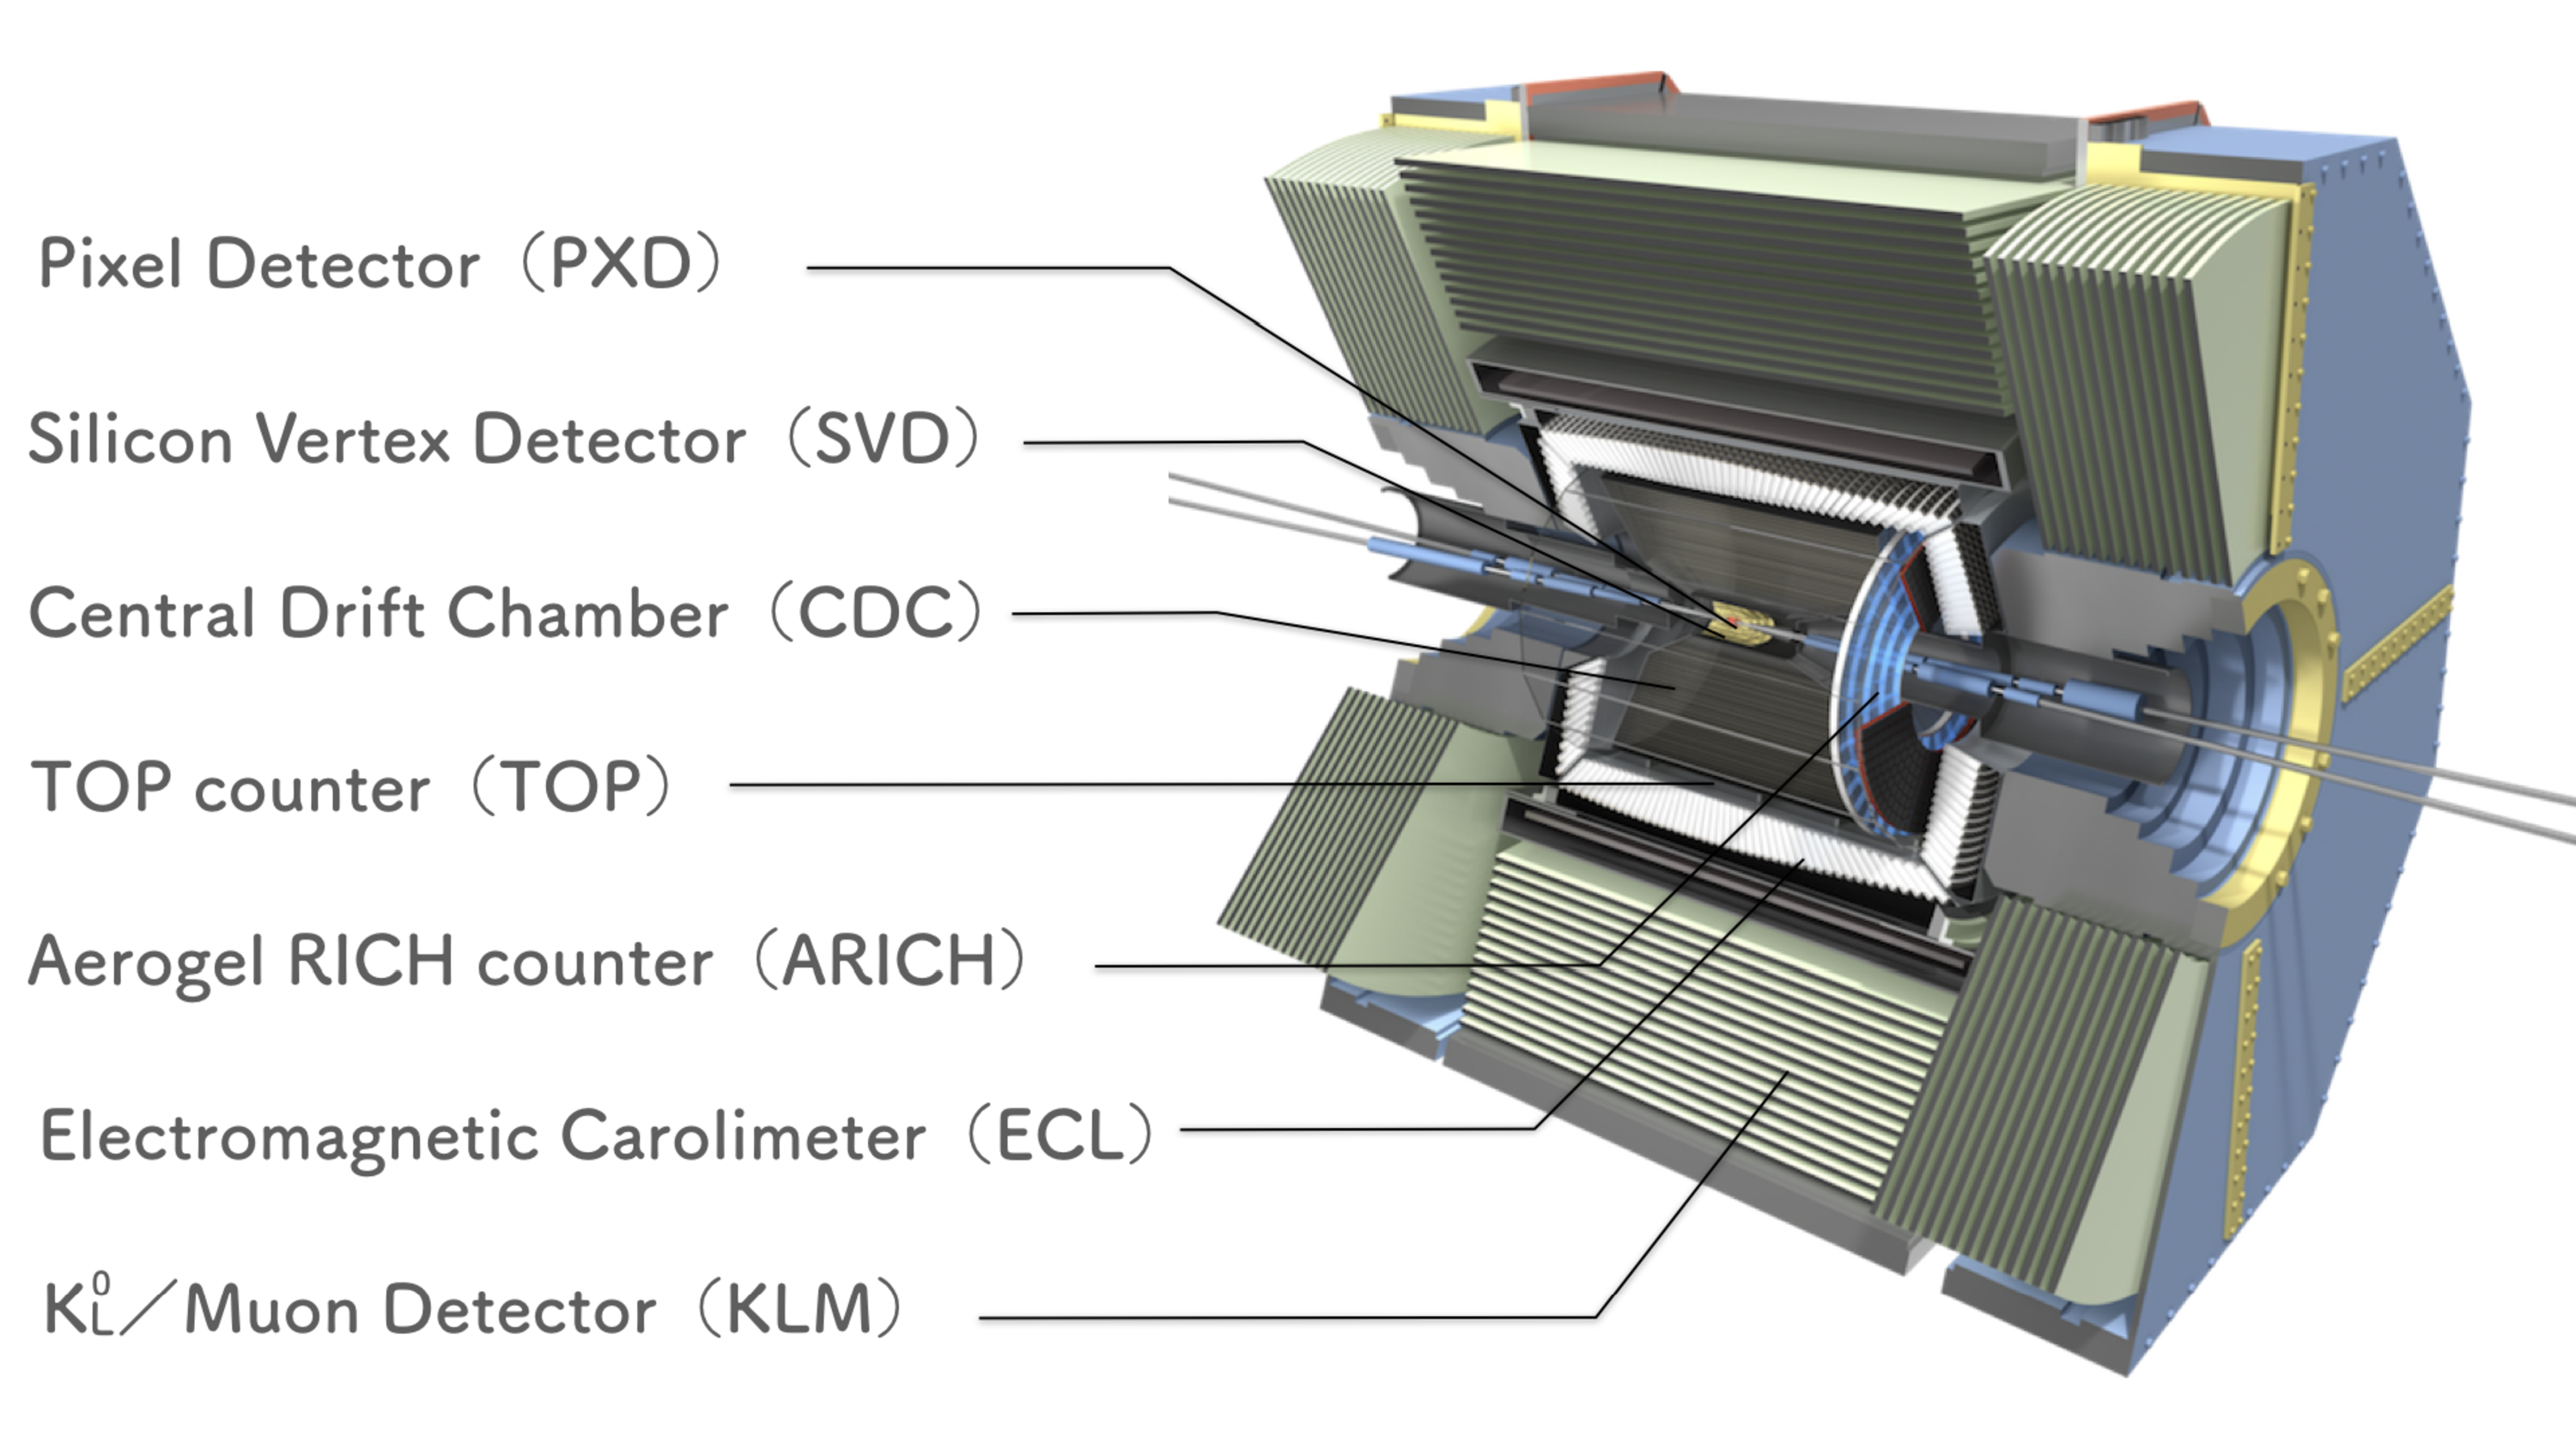
\includegraphics[width=\textwidth]{VBilder/Belle2.pdf}
\end{figure}


	
\end{frame}

\begin{frame}{Vertex Detectors}
	
	
		\begin{textblock*}{10cm}(3cm,-2.3cm)
		\begin{figure}
			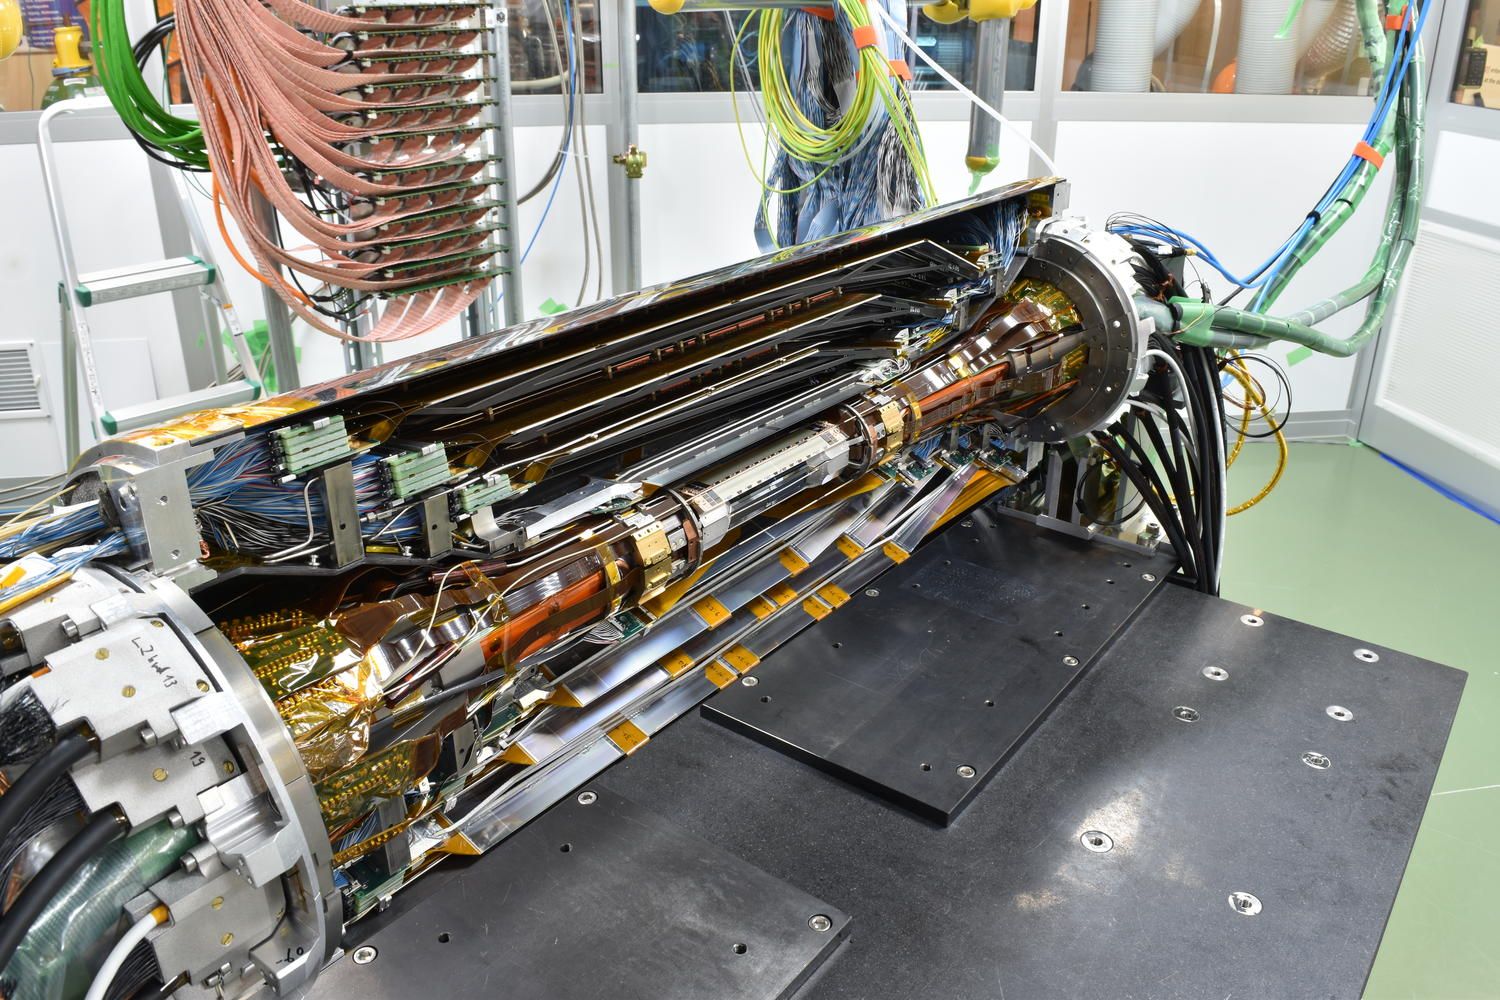
\includegraphics[width=6.5cm]{VBilder/PXD_SVD}
		\end{figure}
		
		
	\end{textblock*}
	
	
	\begin{textblock*}{10cm}(-0cm,-3.7cm)
		Vertex Detectors (VXD):		
			\begin{itemize}
				\item Consist of Pixel Detector (PXD) and Silicon Vertex Detector (SVD)
				\item Both detectors consist of multiple ladders of strip detectors
				\item Charged particles create electron-hole pairs, which are separated by an electric field
				
				The signal is then read out
				\item[] $\rightarrow$ particle position can be determined
			\end{itemize}
		\end{textblock*}
	\begin{textblock*}{5cm}(-0cm,-.6cm)
		\begin{itemize}
	
				\item During phase2, only a fraction of the VXD detectors were installed
				\item During phase3, the complete SVD and roughly half of the PXD are installed
				\item Acceptance: $17.0^{\circ} < \theta < 150.0^{\circ}$ 
			\end{itemize}
		



	\end{textblock*}
	
	

	
	
	
\end{frame}


\begin{frame}{Central Drift Chamber}

	\begin{textblock*}{4cm}(7cm,-2.5cm)
		\begin{figure}
			Axial
			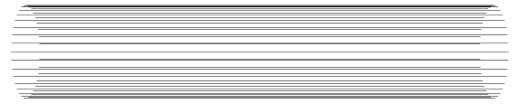
\includegraphics[width=\textwidth]{VBilder/axial}
		\end{figure}
	\end{textblock*}

	\begin{textblock*}{4cm}(7cm,-1.25cm)
		
		\begin{figure}
			Stereo
			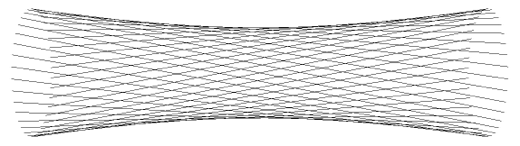
\includegraphics[width=\textwidth]{VBilder/stereo}
		\end{figure}
	\end{textblock*}




	\begin{textblock*}{10cm}(0cm,-3.7cm)
	
		Central Drift Chamber:
		\begin{itemize}
			\item Consists of 14336 sense wires arranged in 5 axial and 4 stereo superlayers (each superlayer consists of 6 layers; with an exception to the innermost superlayer)
			\item Charged particles ionize the gas
			
			The signal is then read out by the sense wires  
			
		\end{itemize}
	\end{textblock*}
	
	
	\begin{textblock*}{6.5cm}(0cm,-1.2cm)
			
		\begin{itemize}	
			\item[] $\rightarrow$ Determination of momenta and tracks of charged particles
			\item Acceptance: $17.0^{\circ} < \theta < 150.0^{\circ}$ 
		\end{itemize}

	\end{textblock*}


\begin{textblock*}{10cm}(0cm,1cm)
	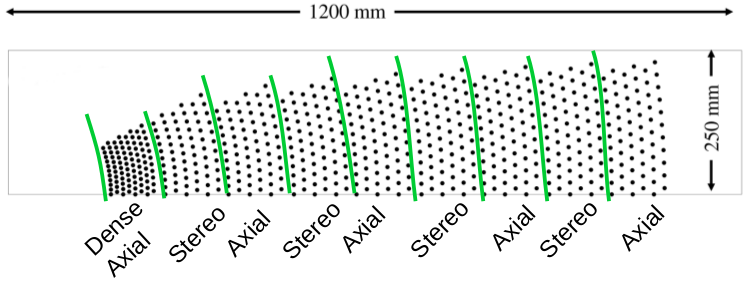
\includegraphics[width=\textwidth]{VBilder/cdc}
\end{textblock*}


\end{frame}


\begin{frame}{Electromagnetic Calorimeter}
	\begin{textblock*}{6cm}(5.5cm,-3.cm)
		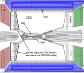
\includegraphics[width=\textwidth]{VBilder/ecl2}
	\end{textblock*}

\begin{textblock*}{5.2cm}(0cm,-3.7cm)
	Electromagnetic Calorimeter:
	\begin{itemize}
		\item Consists of 8936 CsI(Tl) crystals
		\item Electromagnetically interacting particles are  creating electromagnetic cascades when they pass through the crystals
		\item[] $\rightarrow$ clusters are created
		\item[] $\rightarrow$ The position and the energy of the particles can be determined
		\item Separation in \textcolor{blue}{barrel}, \textcolor{OliveGreen}{forward end-cap} and \textcolor{red}{backward end-cap}
		\item There are two $\sim 1^{\circ}$ wide gaps at transition between the sections 
		\item Acceptance: $12.4^{\circ} < \theta < 155.1^{\circ}$ 
	\end{itemize}
\end{textblock*}


\end{frame}

\section{Bhabha Kinematics At Belle II}

\begin{frame}{Bhabha Kinematics At Belle II}
	
	
	

	
	\begin{textblock*}{5.5cm}(6cm,0.cm)
		
		\includegraphics[width=\textwidth]<2>{VBilder/theta_lab}
	\end{textblock*}

	\begin{textblock*}{5.5cm}(0cm,0.0cm)
	
	\includegraphics[width=\textwidth]<2>{VBilder/ee}
\end{textblock*}


	\begin{textblock*}{5cm}(6cm,-3.3cm)
		\begin{itemize}
			\item<2> The beams have asymmetric energies
			
			\item<2> The beams are hitting each other under an angle of $1.26^{\circ}$
			
			$\rightarrow$ Boost the particles from CMS to lab frame
		\end{itemize}
	\end{textblock*}

\begin{textblock*}{5.5cm}(-0.5cm,-3.7cm)
	
	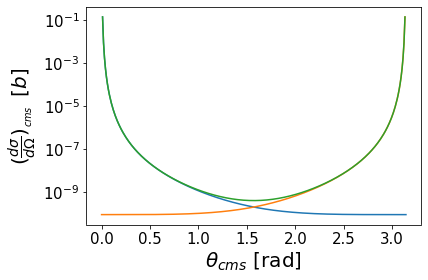
\includegraphics[width=\textwidth]{VBilder/finalCross}
\end{textblock*}




%\begin{textblock*}{2cm}(4.7cm,1.8cm)

%	\begin{tikzpicture}
%		\draw[-{Triangle[width=18pt,length=8pt]}, line width=10pt](0,0) -- (1, 0);
%	\end{tikzpicture}
%	\centering
%	Boost
%\end{textblock*}
	
	

\begin{textblock*}{4cm}(1.1cm,-3.5cm)
	\small{
	\textcolor{blue}{Electrons}
	
	\textcolor{orange}{Positrons}
		
	\textcolor{OliveGreen}{Electrons+Positrons}
}
\end{textblock*}


\begin{textblock*}{4cm}(1.8cm,-3.9cm)
	Cross-Section
\end{textblock*}






\end{frame}





\section{Preparation For Calculating The Tracking Efficiency}





\begin{frame}{Introducing Cuts}
	\begin{textblock*}{11cm}(0cm,-1.7cm)
	\begin{itemize}
		\item<3-> $8\,\textrm{GeV} < \textrm{M}_{\textrm{vpho}} < 12\,\textrm{GeV}$
		\item<3-> 2 clusters with at least $3.5\,\textrm{GeV}$ per event; One cluster has to have at least $4.5\,\textrm{GeV}$
		\item<3-> Number of reconstructed tracks per event $< 7$
		\item<3-> Total energy in the ECL $< 15\,\textrm{GeV}$
	\end{itemize}

\end{textblock*}

\begin{textblock*}{11cm}(0cm,0.5cm)
\begin{figure}[h!]
	\centering
	\pause[4]
	\begin{minipage}[b]{0.45\linewidth}
		\centering
		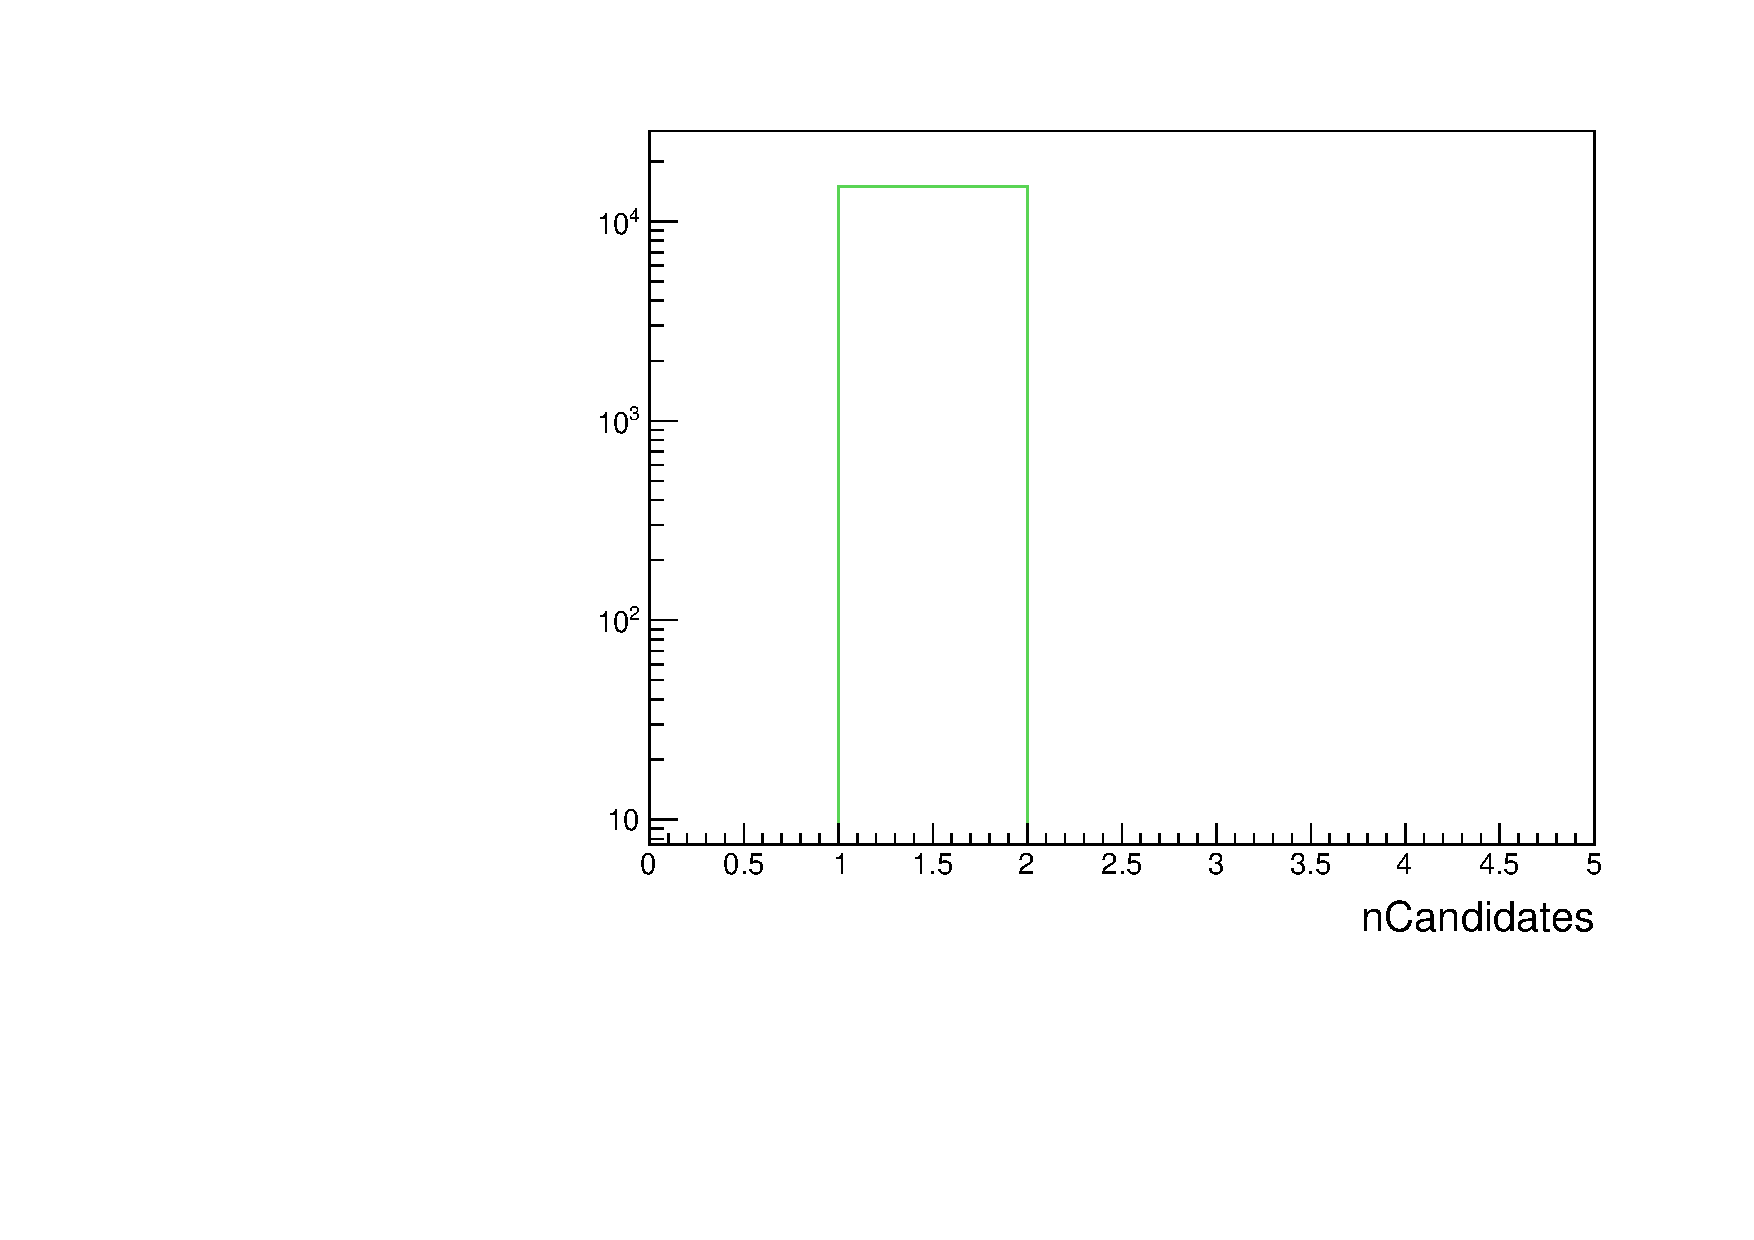
\includegraphics[width=\textwidth]{VBilder/nCandNoMCInfo.pdf}
	\end{minipage}
	\hspace{0.5cm}
	\pause[5]
	\begin{minipage}[b]{0.45\linewidth}
		\centering
		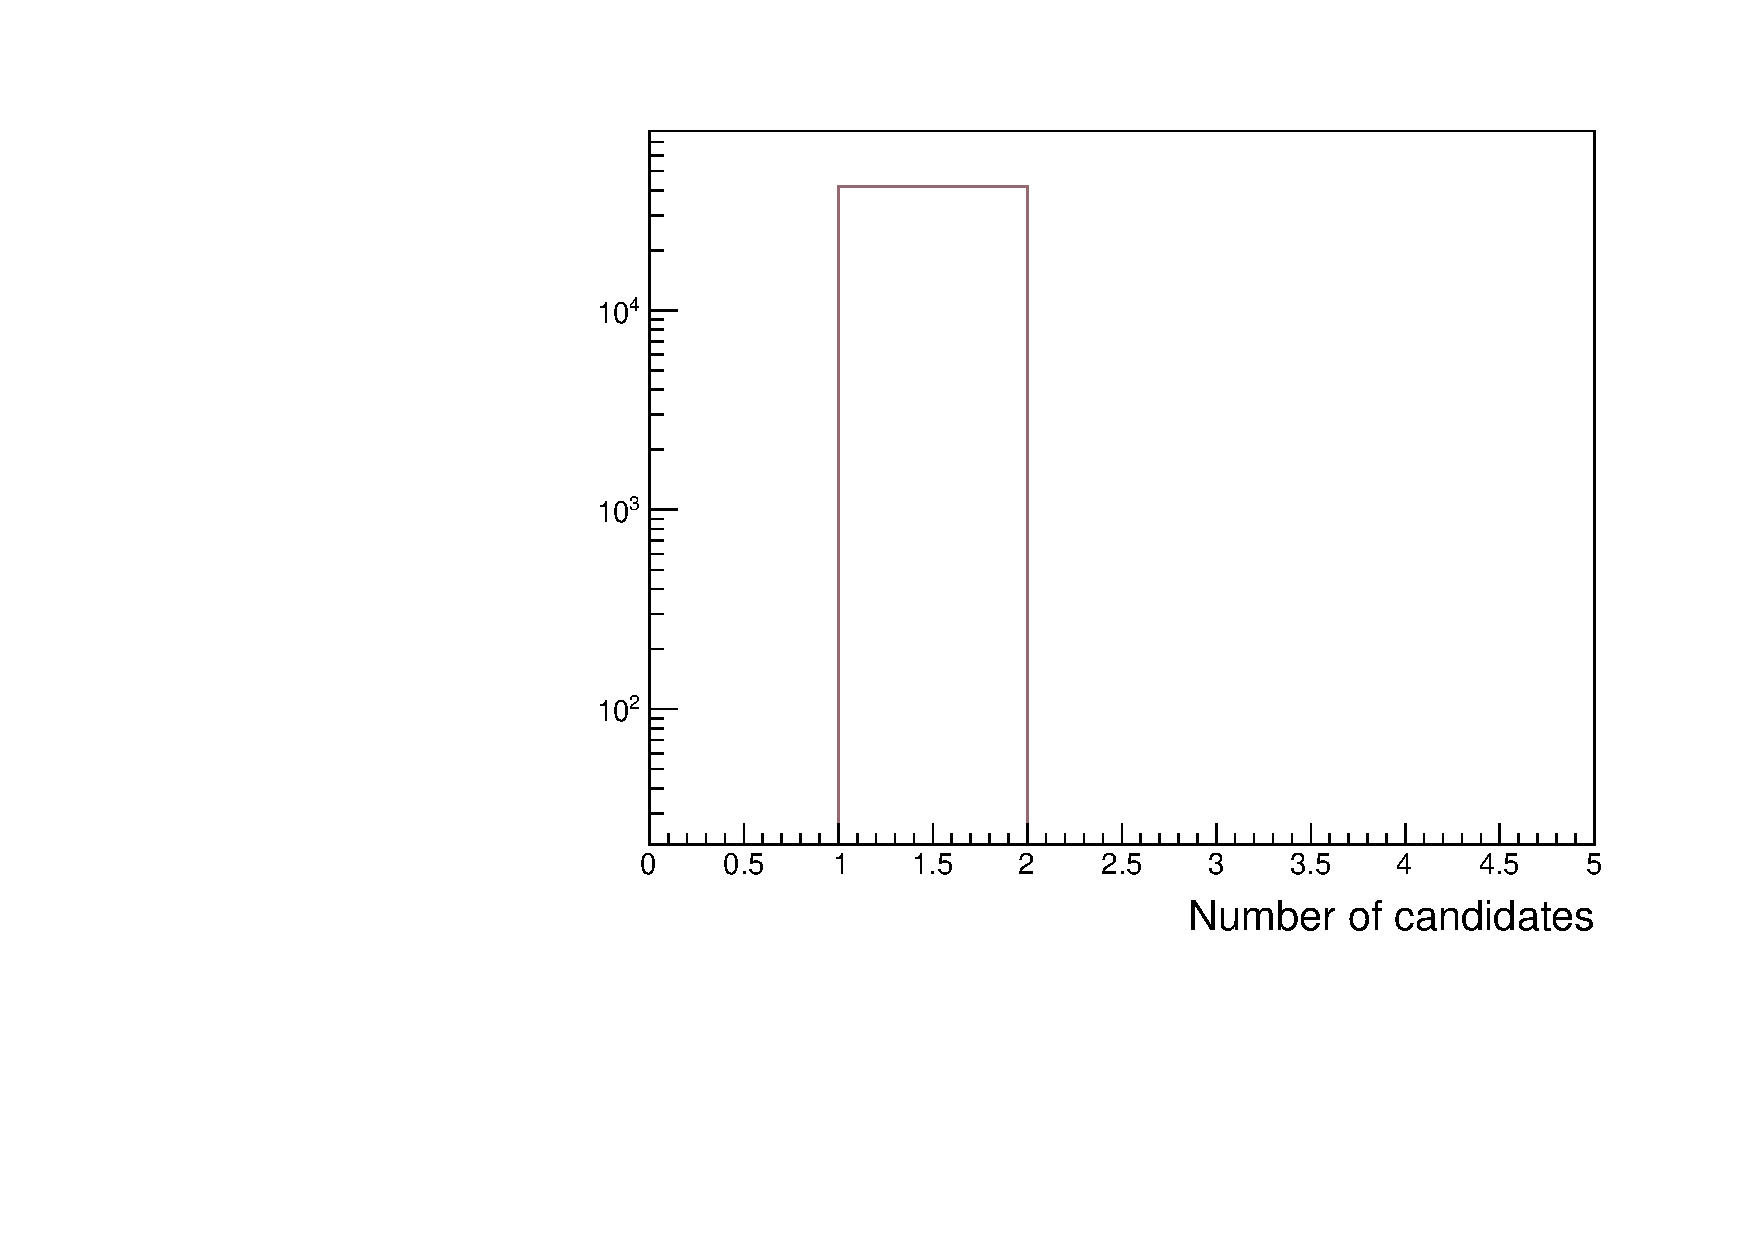
\includegraphics[width=\textwidth]{VBilder/nCandData.pdf}
	\end{minipage}
	
\end{figure}

\end{textblock*}
\pause[4]

\begin{textblock*}{5cm}(0.1cm,0.8cm)
	\centering
	Single phase2 MC10 Bhabha file
\end{textblock*}


\begin{textblock*}{4cm}(2.8cm,1.8cm)
	14581 Events
\end{textblock*}
\pause[5]

\begin{textblock*}{4cm}(8.5cm,1.8cm)
	41853 Events
\end{textblock*}


\begin{textblock*}{4cm}(7.cm,0.8cm)
	Single phase2 data file
\end{textblock*}


\pause[6]



\pause[1]




		


	
\begin{textblock*}{11cm}(0cm,-3.7cm)
				Goal: Reconstruct Bhabha events using only ECL information

	\end{textblock*}
\begin{textblock*}{11cm}(0cm,-3.7cm)	
	\begin{center}
		
		vpho $\rightarrow$ ECL-Object(HclE) + ECL-Object(LclE)		
	\end{center}
\end{textblock*}
\pause[2]
	\begin{textblock*}{11cm}(0cm,-3cm)
	
	\begin{itemize}
		\item[]
		\item The particles have to pass the tracking detectors
		\item[] $\rightarrow$ $17.0^{\circ} < \theta_{\textrm{ECL-Object}} < 150.0^{\circ}$

	\end{itemize}	
\end{textblock*}


\pause[1]
\begin{textblock*}{11cm}(0cm,-3.3cm)
	\begin{center}
		\footnotesize{HclE: particle with higher cluster Energy; LclE: particle with lower cluster Energy}
	\end{center}
\end{textblock*}

\pause[6]
\begin{textblock*}{5cm}(3.2cm,0cm)
	\begin{tikzpicture}[node distance=3cm]
	
	% nodes
	\node (A) at (3, 0) {};
	\node (B) at (1, 2) {\textcolor{white}{Also contains $\textrm{ee}\rightarrow\gamma \gamma$ events}};
	\draw[<-, to path={-| (\tikztotarget)}]
	(A) edge (B);
	
	\end{tikzpicture}
	

\end{textblock*}

\pause[6]




\begin{textblock*}{5cm}(3.2cm,-0.4cm)
	
\begin{mybox}
Also contains $\textrm{ee}\rightarrow\gamma \gamma$ events	
\end{mybox}

\end{textblock*}




\end{frame}



\begin{frame}{Bhabha Event Selection}
	
	\begin{figure}
		\centering
		\includegraphics<1>[width=\textwidth]{Plots/b2b_2}
	\end{figure}
	
\end{frame}

\begin{frame}{Bhabha Event Selection}
	
	\begin{textblock*}{0.5\textwidth}(0cm,-3cm)
		\centering
		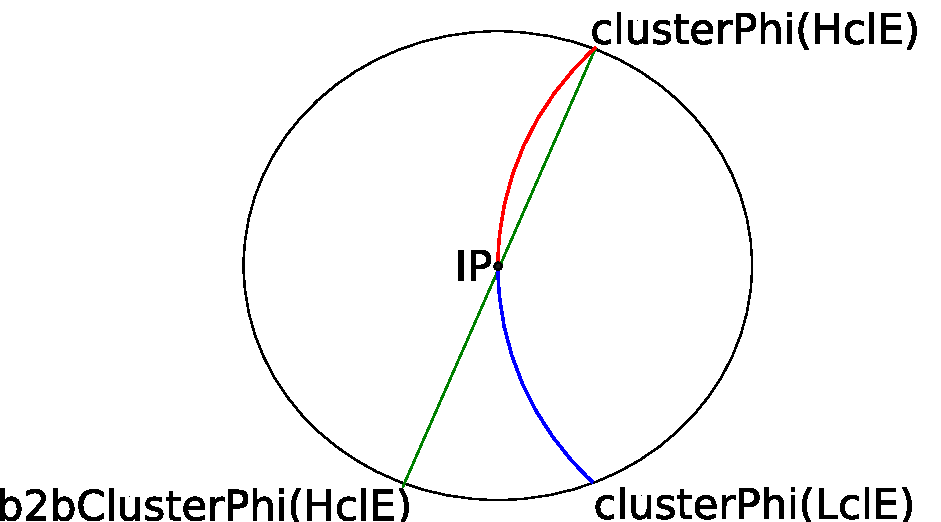
\includegraphics[width=4.5cm]{VBilder/b2b_2}
	\end{textblock*}
	
	\begin{textblock*}{0.5\textwidth}(5.5cm,-3cm)
		\centering
		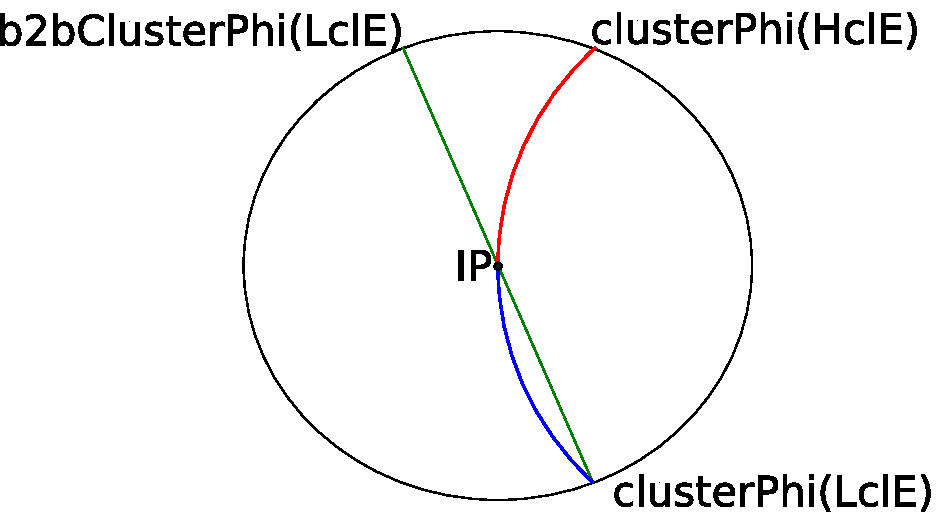
\includegraphics[width=4.5cm]{VBilder/b2b_3}
	\end{textblock*}
	
	
	\begin{textblock*}{1\textwidth}(0cm,0.cm)
		\centering
		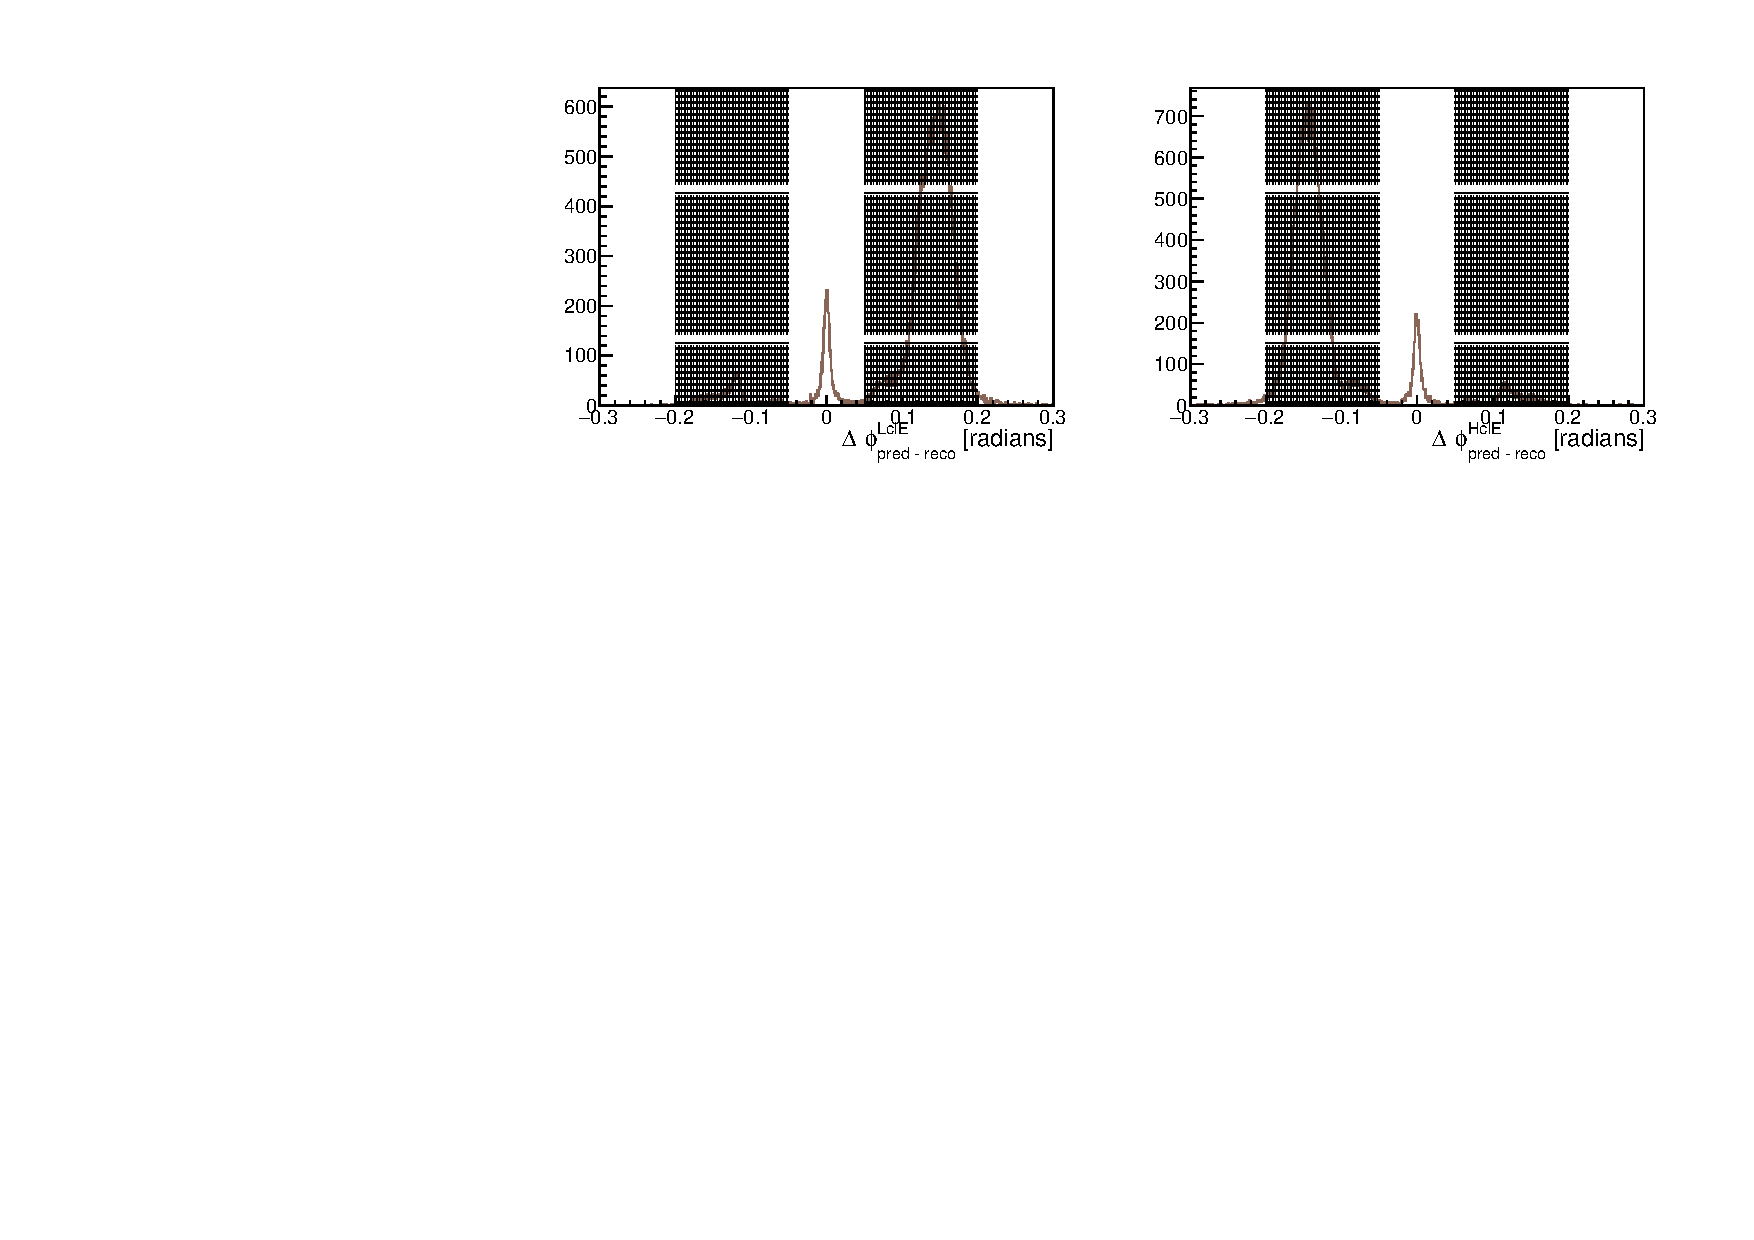
\includegraphics[width=\textwidth]{VBilder/sb2b_Data.pdf}
	\end{textblock*}
	
	
\pause	
	
		\begin{textblock*}{1\textwidth}(0cm,0.cm)
		\centering
		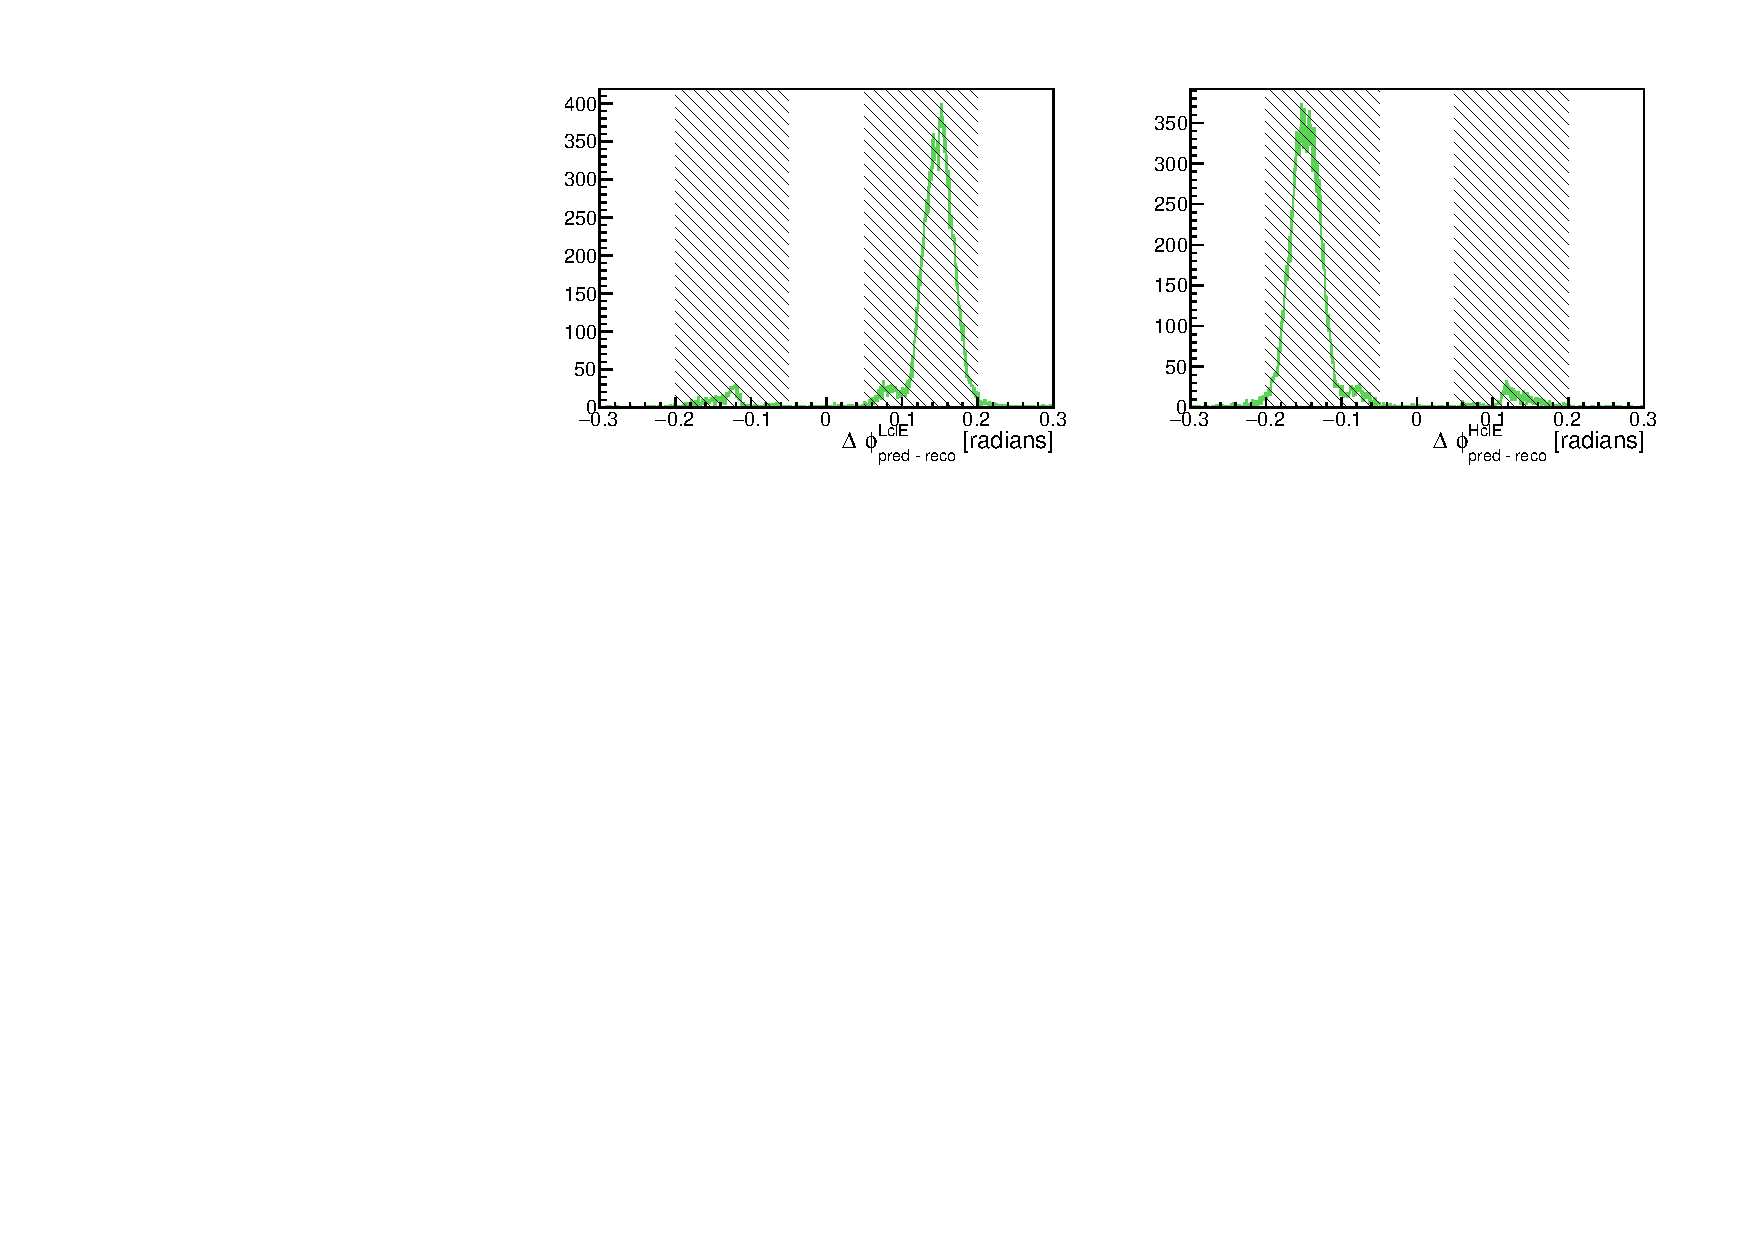
\includegraphics[width=\textwidth]{VBilder/sb2b_MC.pdf}
	\end{textblock*}
	
	

	
\end{frame}


\begin{frame}{Trigger}
	
	\begin{textblock*}{6.5cm}(5.5cm,-0.cm)
		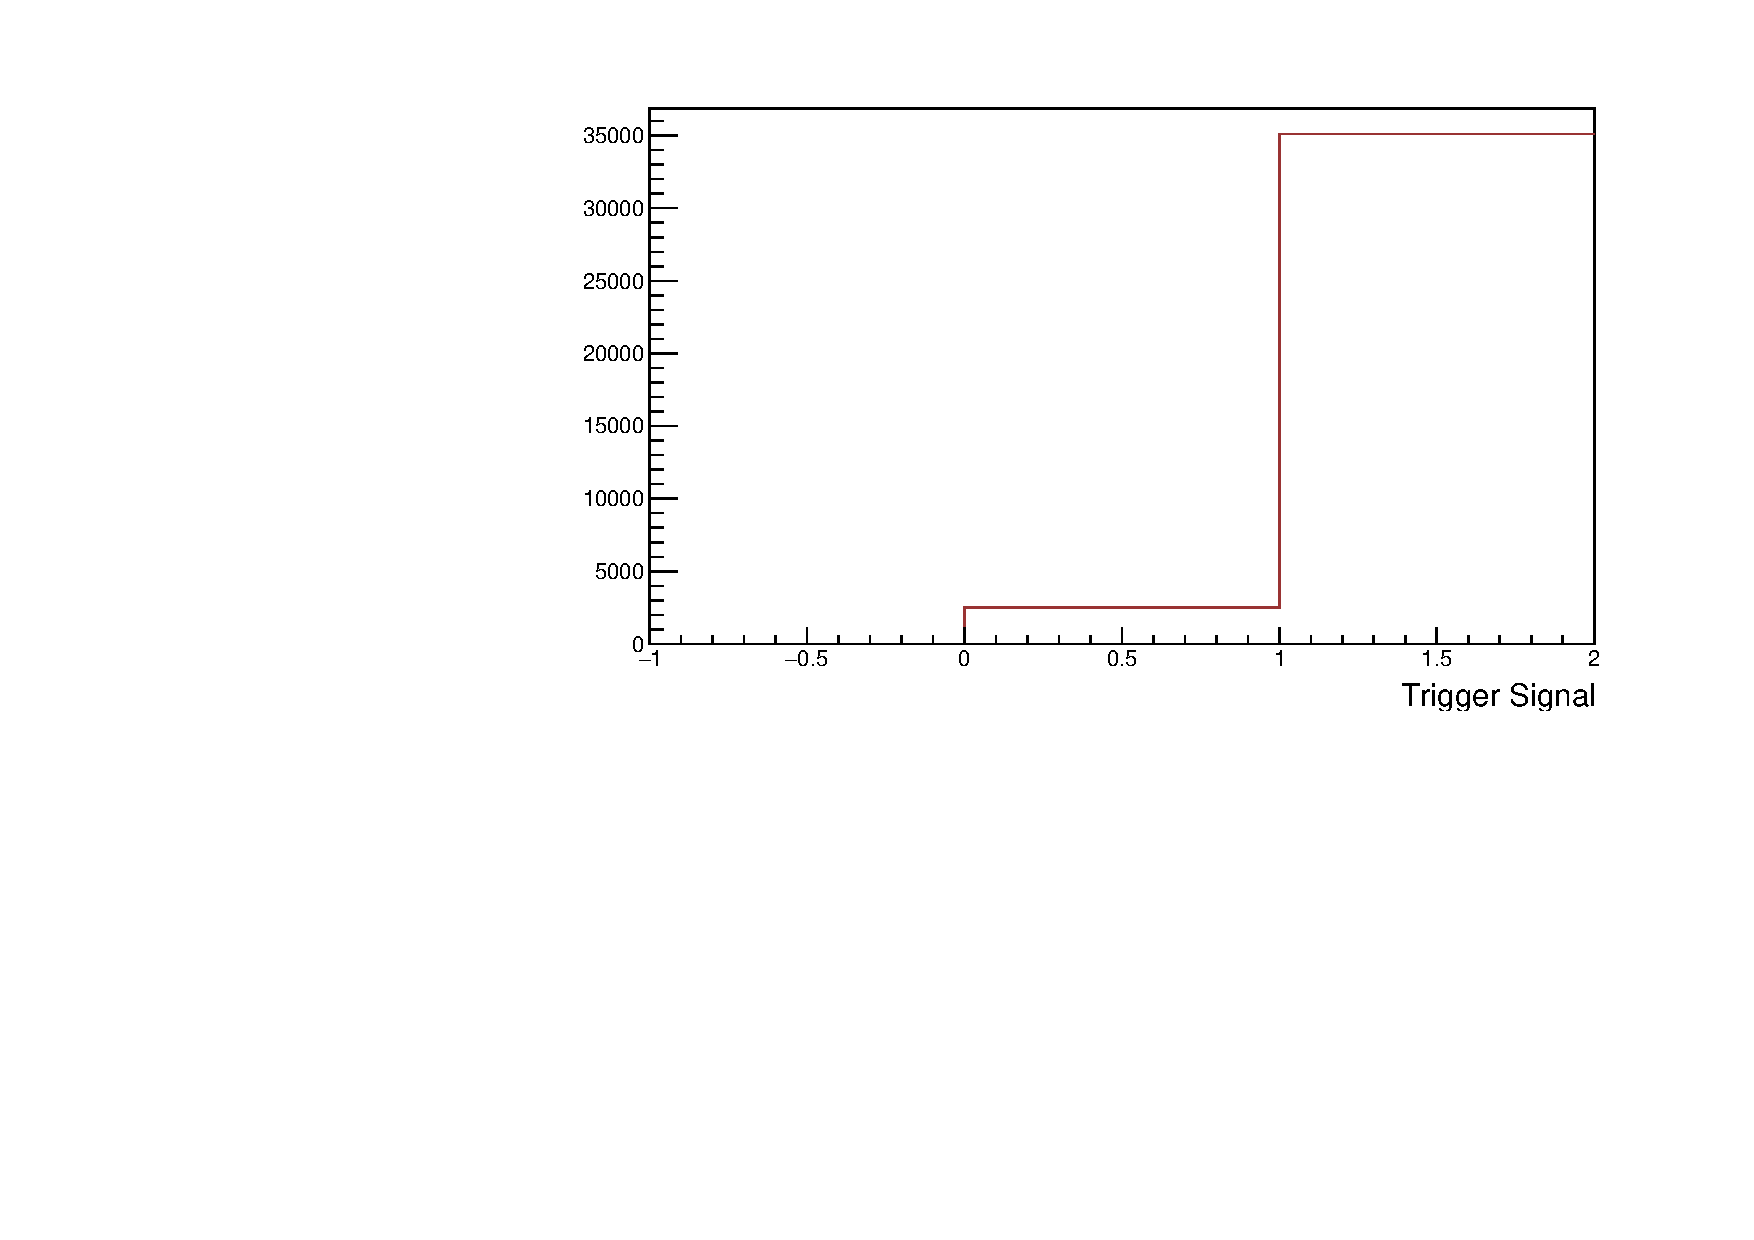
\includegraphics[width=\textwidth]{VBilder/DataTrigger}
	\end{textblock*}
	
	
	
	
	
	\begin{textblock*}{11cm}(0cm,-2.9cm)
		
		We need to be sure that a trigger signal is coming from the ECL 
		
		Otherwise there could be a bias
		
		$\rightarrow$ The \texttt{bhabha} trigger bit is used
		
		This trigger requires several conditions:
		\begin{itemize}
			\item Trigger signal coming from the ECL
			\item Both reconstructed particles have to have a cluster energy of at least $2.5\,\textrm{GeV}$ each and one has to have at least $4\,\textrm{GeV}$
			\item $160^{\circ} < \sum \theta_{cms} < 200^{\circ}$
			\item $140^{\circ} < \Delta \phi_{cms} < 220^{\circ}$
		
		\end{itemize}
	
\end{textblock*}
	
	
	
	
	\begin{textblock*}{5.5cm}(0cm,1.9cm)
	
	The trigger cut will not be applied to MC since the trigger simulation does not work reliably on MC 
	\end{textblock*}
\end{frame}





\begin{frame}{Dividing The ECL In Areas Of Interest}
	
	\begin{textblock*}{5cm}(-0.3cm,-3.7cm)
		As function of azimuthal angle $\phi_{\textrm{pred,b2b}}$
	\end{textblock*}
	\pause[1]
	\begin{textblock*}{5cm}(-0.3cm,-3.4cm)
	\begin{table}[h!]
		\centering
		\begin{tabular}{lc}
			&p($\textrm{e}^-$)\\
			\hline
			Forward End-Cap & \pause[2]$4\,\textrm{GeV} - 8\,\textrm{GeV}$\\
			\pause[1]Barrel &\pause[2] $4\,\textrm{GeV} - 7\,\textrm{GeV}$\\
			\pause[1]Backward End-Cap &\pause[2] /\\	
		\end{tabular}

	\end{table}
	
	
\end{textblock*}
	\pause[1]
	
	\begin{textblock*}{6.5cm}(5cm,-4cm)
		\includegraphics[width=\textwidth]<1>{VBilder/em_1}
		\includegraphics[width=\textwidth]<2>{VBilder/em_2}
		\includegraphics[width=\textwidth]<3,4>{VBilder/RTPMemD_MC}
	\end{textblock*}
	
	\pause[5]
	
	\begin{textblock*}{5cm}(-0.3cm,-1.6cm)
		
		
		\begin{table}[h!]
			\centering
			\begin{tabular}{lc}
				&p($\textrm{e}^+$)\\
				\hline
				Forward End-Cap &/\\
				Barrel &$3\,\textrm{GeV} - 7\,\textrm{GeV}$\\
				Backward End-Cap & $2\,\textrm{GeV} - 6\,\textrm{GeV}$\\	
			\end{tabular}

		\end{table}
		
	\end{textblock*}
	
	
	\begin{textblock*}{6.5cm}(5cm,-4cm)
		\includegraphics[width=\textwidth]<5>{VBilder/RTPMepD_MC}
	\end{textblock*}
	
	
	\pause[4]
	
	\begin{textblock*}{5cm}(-0.3cm,1.5cm)
	As function of polar angle $\theta_{\textrm{pred,b2b}}$
\end{textblock*}
\begin{textblock*}{5cm}(-0.3cm,1.5cm)
	\begin{table}[h!]
		\centering
		\begin{tabular}{lc}
			&p\\
			\hline
			$\textrm{e}^-$& $4\,\textrm{GeV} - 9\,\textrm{GeV}$\\	
			\pause[5]
			$\textrm{e}^+$& $2\,\textrm{GeV} - 7\,\textrm{GeV}$\\	
		\end{tabular}
		
	\end{table}
\end{textblock*}









\end{frame}




%-----------------------------------------------------
\section{Phase3 Tracking Efficiencies}

\begin{frame}{Phase3 Tracking Efficiencies As Function Of $\theta_{\textrm{pred,b2b}}-\phi_{\textrm{pred,b2b}}$}
	
	
	
	\begin{textblock*}{9cm}(1cm,-4cm)
		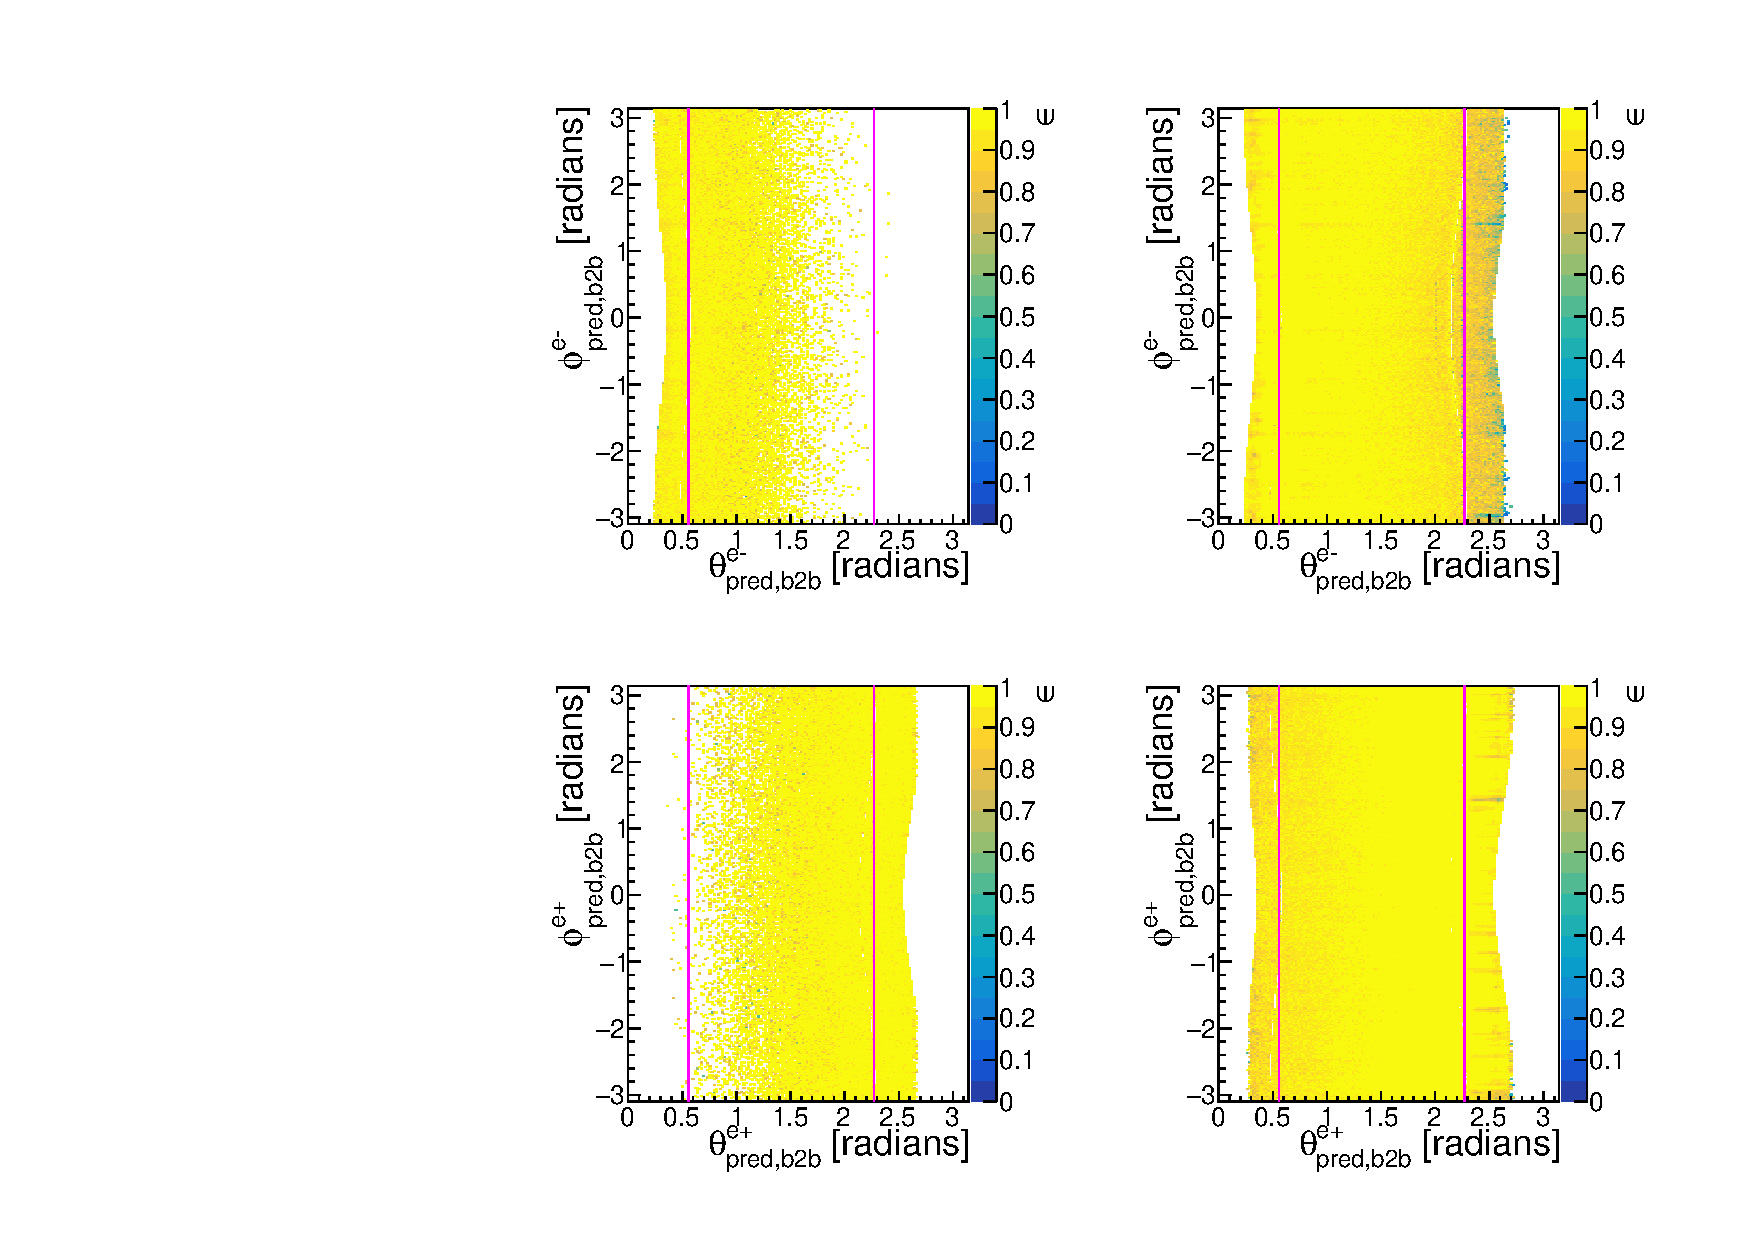
\includegraphics[width=\textwidth]{VPlots/P3/xCEffTP_MCDataP3}
	\end{textblock*}
	
	\begin{textblock*}{2cm}(0cm,-2cm)
		$\textrm{e}^-$
	\end{textblock*}
	
	\begin{textblock*}{2cm}(0cm,2.3cm)
		$\textrm{e}^+$
	\end{textblock*}
	
	
	\begin{textblock*}{2cm}(2.8cm,-3.9cm)
		MC
	\end{textblock*}
	
	\begin{textblock*}{2cm}(7.2cm,-3.9cm)
		Data
	\end{textblock*}
	
	
	\begin{textblock*}{8cm}(1.5cm,0.8cm)
		\only<2>{
			
			\begin{mybox}
				For phase3 data there are electron tracking efficiency drops in the forward end-cap and in the barrel
				
			\end{mybox}
			
		}
		
	\end{textblock*}
	
	
	
		\begin{textblock*}{8cm}(1.5cm,-1.1cm)
		\only<3>{
			
			\begin{mybox}
				The same kind of drops are also visible in the positron tracking efficiency in the backward end-cap 				
				
			\end{mybox}
			
		}
		
	\end{textblock*}
	
	
	
	
	
\end{frame}





\begin{frame}{Phase3 Tracking Efficiencies As Function Of $\theta_{\textrm{pred,b2b}}$}
	
	
	\begin{textblock*}{6.5cm}(-0.9cm,-3cm)
		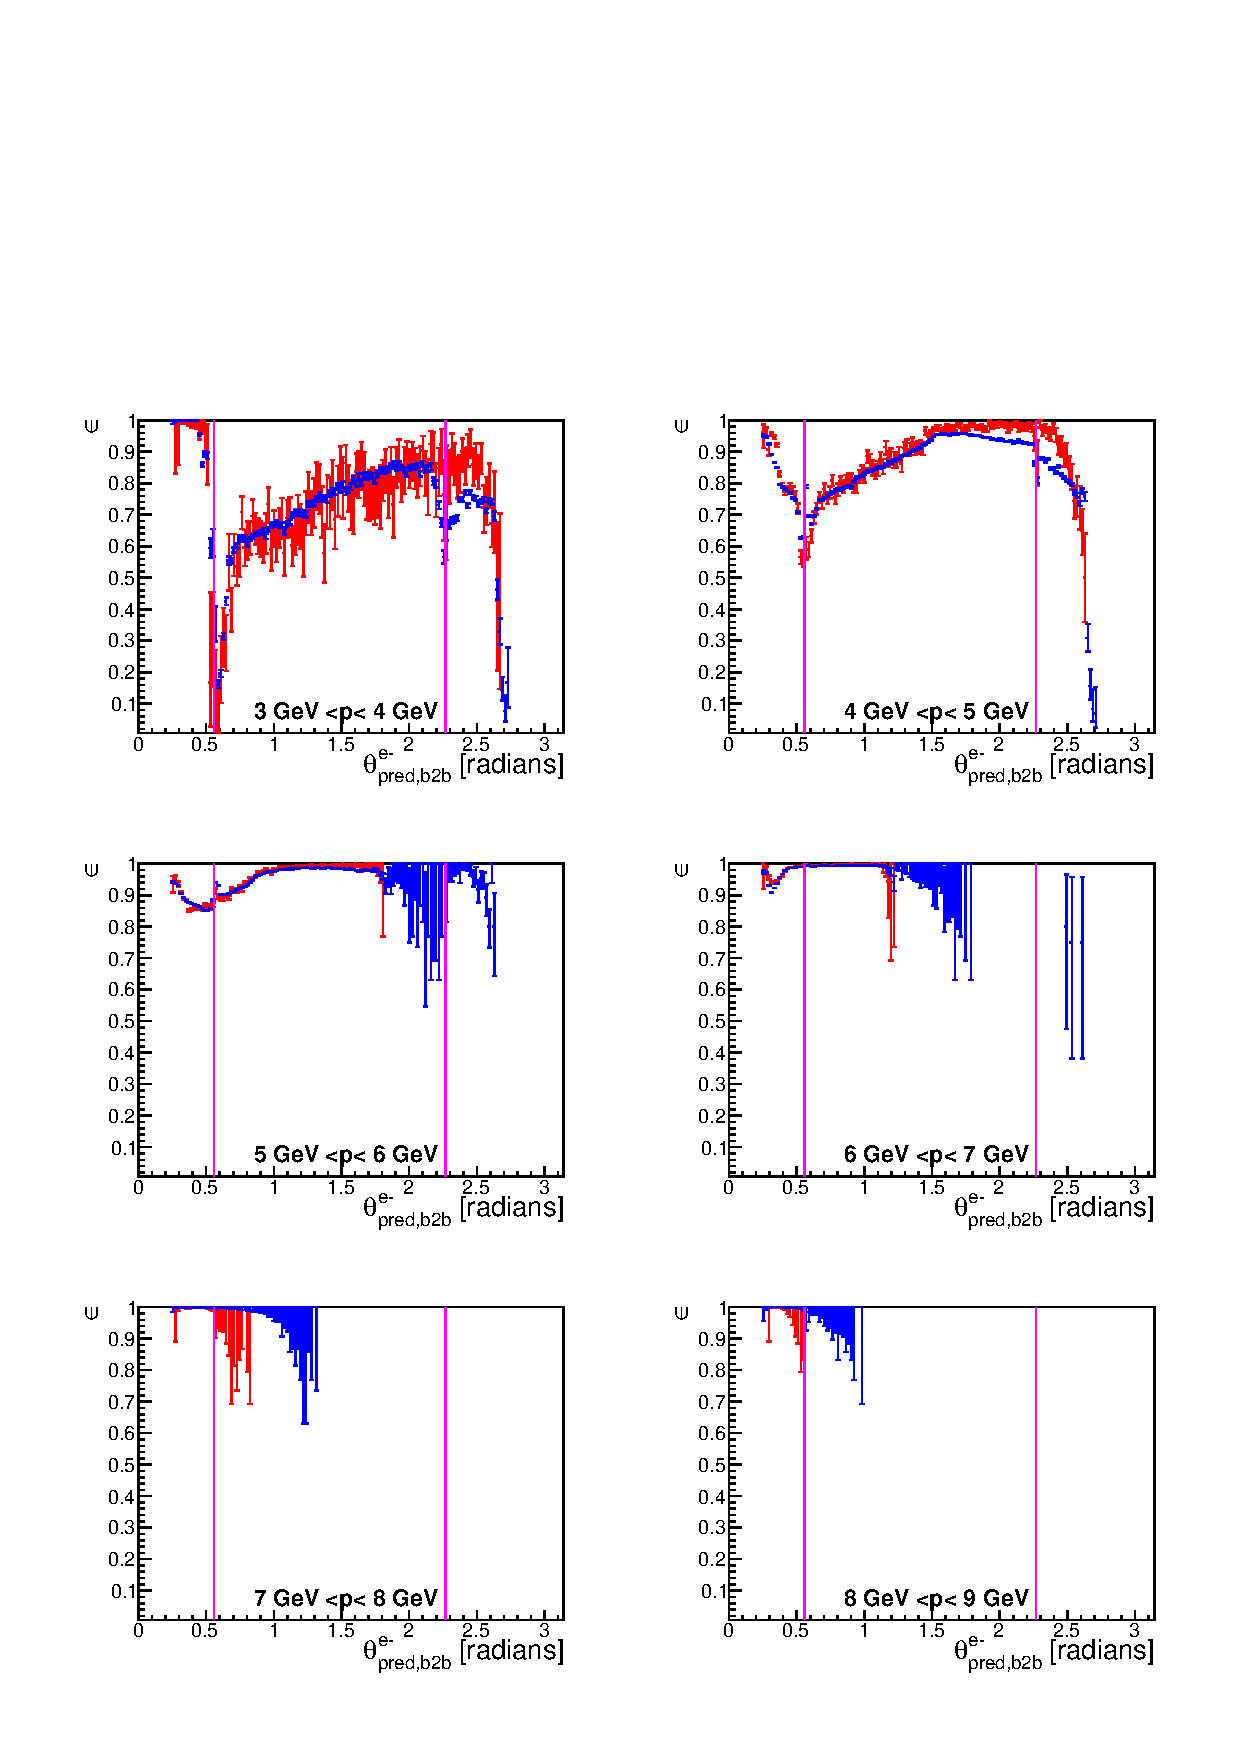
\includegraphics[width=\textwidth]{VPlots/P3/xPMThetaemP3}
	\end{textblock*}
	
	\begin{textblock*}{6.5cm}(5.5cm,-3cm)
		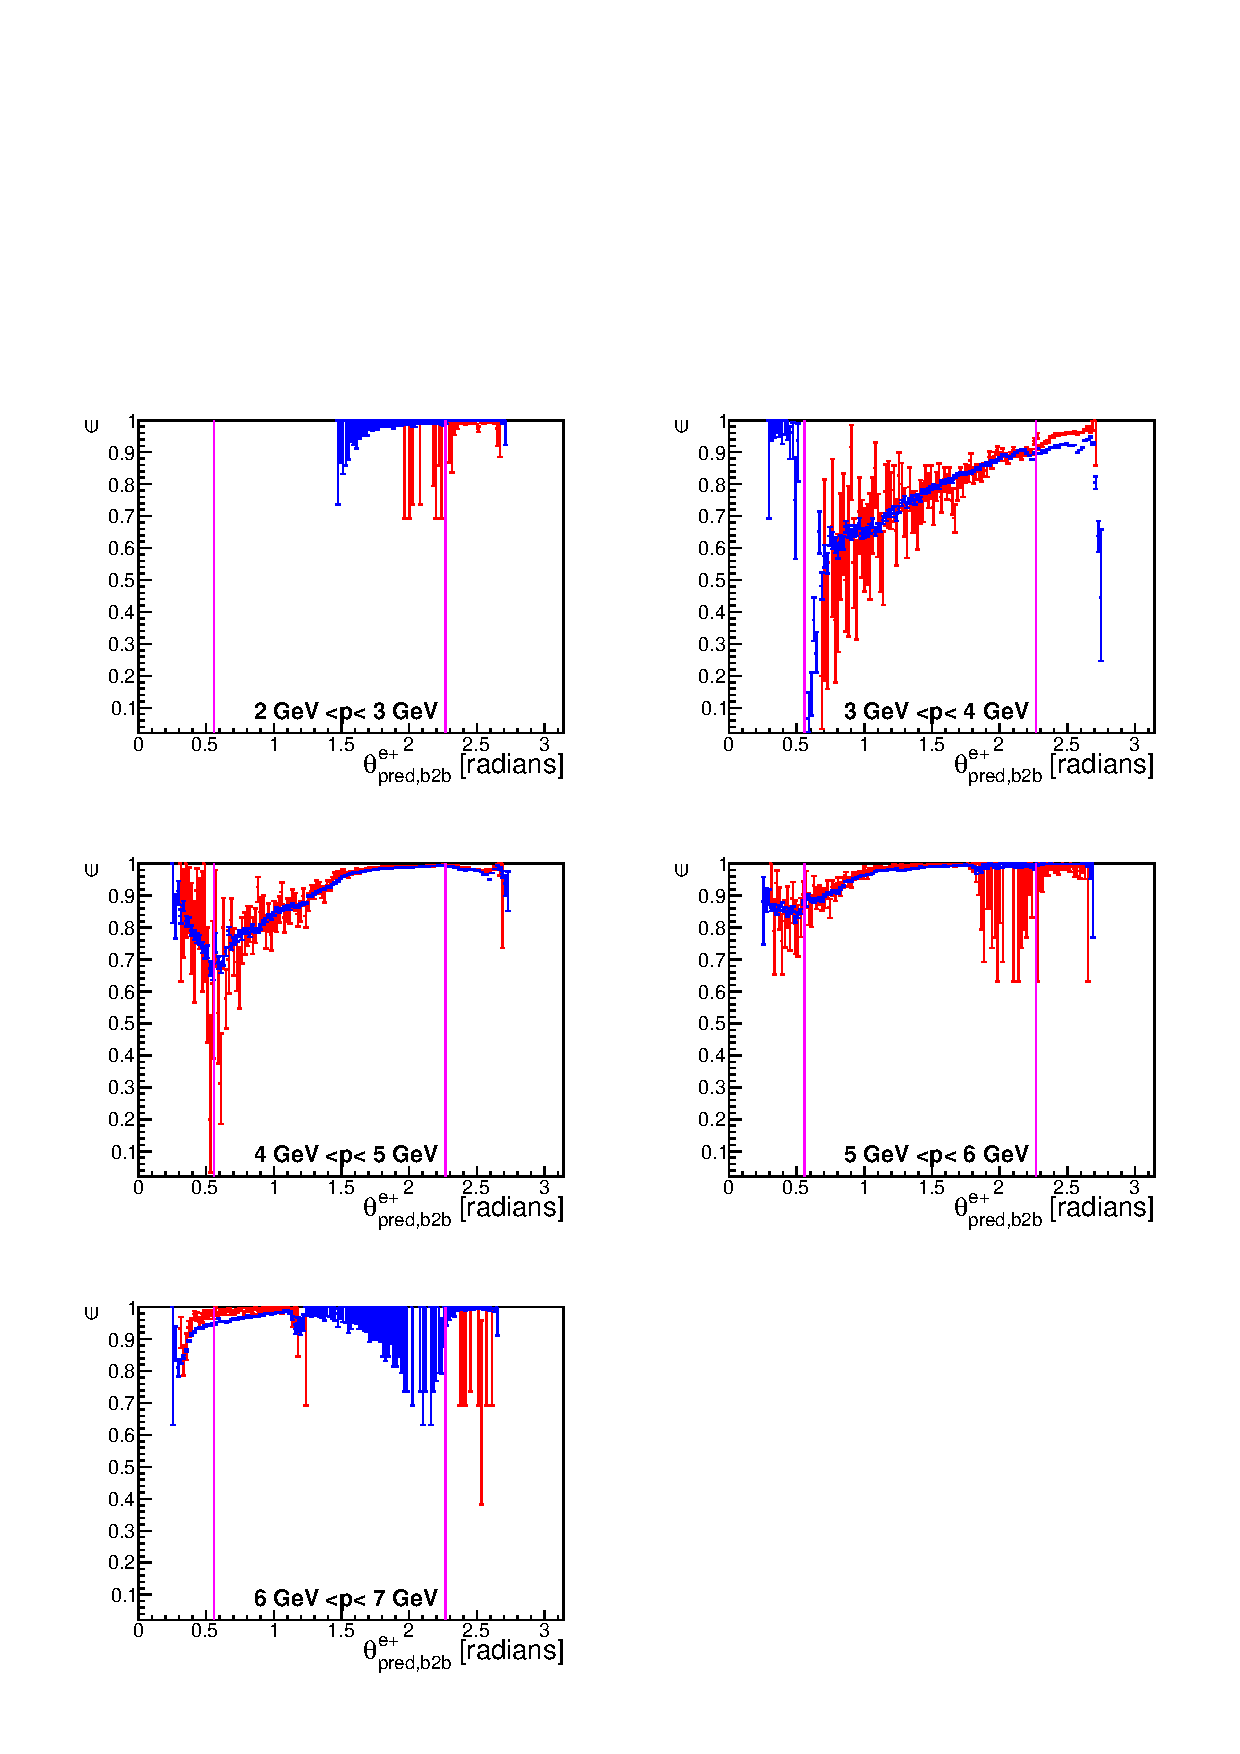
\includegraphics[width=\textwidth]{VPlots/P3/xPMThetaepP3}
	\end{textblock*}
	
	
	\begin{textblock*}{2cm}(2.3cm,-3.5cm)
		$\textrm{e}^-$
	\end{textblock*}
	
	\begin{textblock*}{2cm}(8.7cm,-3.5cm)
		$\textrm{e}^+$
	\end{textblock*}
	
	
	
	\begin{textblock*}{11cm}(5.5cm,-4.3cm)
		
		\begin{center}
			\line(0,1){256}
		\end{center}
		
	\end{textblock*}
	
	
	
	\only<1,2,3,4,5,6>{
		
		
		\begin{textblock*}{4cm}(-0.5cm,-3.7cm)
			\textcolor{red}{Phase3 MC10}
			
			\textcolor{blue}{Phase3 Data}
		\end{textblock*}
		
	}
	
	\only<7->{
		
		
		\begin{textblock*}{4cm}(6cm,-3.7cm)
			\textcolor{red}{Phase3 MC10}
			
			\textcolor{blue}{Phase3 Data}
		\end{textblock*}
		
	}
	
	\only<2,3,4,5,6>{
		\begin{textblock*}{6cm}(5.6cm,-3.5cm)
			\begin{mybox}
				Electron Tracking Efficiency:
				\begin{itemize}
					\item Phase3 MC and phase3 data are very close to each other (exception occurs for momenta between $4\,\textrm{GeV}$ and $5\,\textrm{GeV}$) 
					\item<4->  Efficiency drops at transition between barrel and end-caps
					\item<5-> There is a slope in the barrel
					
				\end{itemize}
			\end{mybox}
		\end{textblock*}
	}
	
	\begin{textblock*}{5cm}(4.0cm,-2.8cm)
		\begin{tikzpicture}
		\only<3>{
			\draw[line width=0.5mm,winered] \boundellipse{2cm,0cm}{.5cm}{.3cm};
		}
		\end{tikzpicture}
	\end{textblock*}
	
	
	
	
		\begin{textblock*}{5cm}(1.cm,-2.8cm)
		\begin{tikzpicture}
		\only<3>{
			\draw[line width=0.5mm,winered] \boundellipse{2cm,0cm}{.3cm}{.5cm};
		}
		\end{tikzpicture}
	\end{textblock*}
	
	
	
	
	
	
	
	
	
	
	\begin{textblock*}{5cm}(-0.2cm,-2.8cm)
		\begin{tikzpicture}
		\only<4>{
			\draw[line width=0.5mm,winered] \boundellipse{2cm,0cm}{0.2cm}{1.cm};
		}
		\end{tikzpicture}
	\end{textblock*}
	
	
	
	\begin{textblock*}{5cm}(1.1cm,-2.8cm)
		\begin{tikzpicture}
		\only<4>{
			\draw[line width=0.5mm,winered] \boundellipse{2cm,0cm}{0.2cm}{1.cm};
		}
		\end{tikzpicture}
	\end{textblock*}
	
	
	
	\begin{textblock*}{5cm}(3.1cm,-2.8cm)
		\begin{tikzpicture}
		\only<4>{
			\draw[line width=0.5mm,winered] \boundellipse{2cm,0cm}{0.2cm}{1.cm};
		}
		\end{tikzpicture}
	\end{textblock*}	
	
	\begin{textblock*}{5cm}(4.35cm,-2.8cm)
		\begin{tikzpicture}
		\only<4>{
			\draw[line width=0.5mm,winered] \boundellipse{2cm,0cm}{0.2cm}{1.cm};
		}
		\end{tikzpicture}
	\end{textblock*}
	
	
	
	\begin{textblock*}{5cm}(.cm,-2.7cm)
		\begin{tikzpicture}
		\only<5>{
			\draw[line width=0.5mm,winered] \boundellipse{2cm,0cm}{.7cm}{.5cm};
		}
		\end{tikzpicture}
	\end{textblock*}
	
	
	
	\begin{textblock*}{5cm}(3.2cm,-2.7cm)
		\begin{tikzpicture}
		\only<5>{
			\draw[line width=0.5mm,winered] \boundellipse{2cm,0cm}{.5cm}{.3cm};
		}
		\end{tikzpicture}
	\end{textblock*}
	
	
	\begin{textblock*}{5cm}(-.1cm,-.4cm)
		\begin{tikzpicture}
		\only<5>{
			\draw[line width=0.5mm,winered] \boundellipse{2cm,0cm}{.3cm}{.3cm};
		}
		\end{tikzpicture}
	\end{textblock*}
	
	\pause[6]
	
	
	\begin{textblock*}{6cm}(-0.7cm,-3.5cm)
		
		\only<7->{
			\begin{mybox}
				Positron Tracking Efficiency:
				\begin{itemize}
					
					\item The tracking efficiency pf phase3 MC and phase3 data are close to each other (exception occurs in the backward end-cap for momenta between $2\,\textrm{GeV}$ and $4\,\textrm{GeV}$ and between $6\,\textrm{GeV}$ and $7\,\textrm{GeV}$) 
					\item<9->Efficiency drops at transition between barrel and end-caps
					\item<10-> There is a slope in the barrel
					
				\end{itemize}
			\end{mybox}
		}
	\end{textblock*}
	
	
	\begin{textblock*}{5cm}(10.8cm,-2.8cm)
		\begin{tikzpicture}
		\only<8>{
			\draw[line width=0.5mm,winered] \boundellipse{2cm,0cm}{.3cm}{.3cm};
		}
		\end{tikzpicture}
	\end{textblock*}


	\begin{textblock*}{5cm}(6.1cm,2cm)
		\begin{tikzpicture}
		\only<8>{
			\draw[line width=0.5mm,winered] \boundellipse{2cm,0cm}{.4cm}{.3cm};
		}
		\end{tikzpicture}
	\end{textblock*}
	

	
	\begin{textblock*}{5cm}(6.1cm,-0.4cm)
		\begin{tikzpicture}
		\only<9>{
			\draw[line width=0.5mm,winered] \boundellipse{2cm,0cm}{0.3cm}{1.cm};
		}
		\end{tikzpicture}
	\end{textblock*}
	
	
		
	\begin{textblock*}{5cm}(9.4cm,-2.8cm)
		\begin{tikzpicture}
		\only<9>{
			\draw[line width=0.5mm,winered] \boundellipse{2cm,0cm}{0.3cm}{1.cm};
		}
		\end{tikzpicture}
	\end{textblock*}
	
	
	
	
	
	
	
	\begin{textblock*}{5cm}(9.5cm,-2.8cm)
		\begin{tikzpicture}
		\only<10>{
			\draw[line width=0.5mm,winered] \boundellipse{2cm,0cm}{0.8cm}{0.7cm};
		}
		\end{tikzpicture}
	\end{textblock*}
	
	
	
	\begin{textblock*}{5cm}(9.5cm,-0.4cm)
		\begin{tikzpicture}
		\only<10>{
			\draw[line width=0.5mm,winered] \boundellipse{2cm,0cm}{0.4cm}{0.3cm};
		}
		\end{tikzpicture}
	\end{textblock*}
	
	\begin{textblock*}{5cm}(6.3cm,-0.3cm)
		\begin{tikzpicture}
		\only<10>{
			\draw[line width=0.5mm,winered] \boundellipse{2cm,0cm}{0.6cm}{0.4cm};
		}
		\end{tikzpicture}
	\end{textblock*}	
	
	
	
	
	
	\pause[11]
	
	
	
	
	
	
	
	
\end{frame}

















\begin{frame}{Phase3 Tracking Efficiencies As Function Of $\phi_{\textrm{pred,b2b}}$; Forward End-Cap}
	
	
	\begin{textblock*}{6.5cm}(-0.9cm,-3cm)
		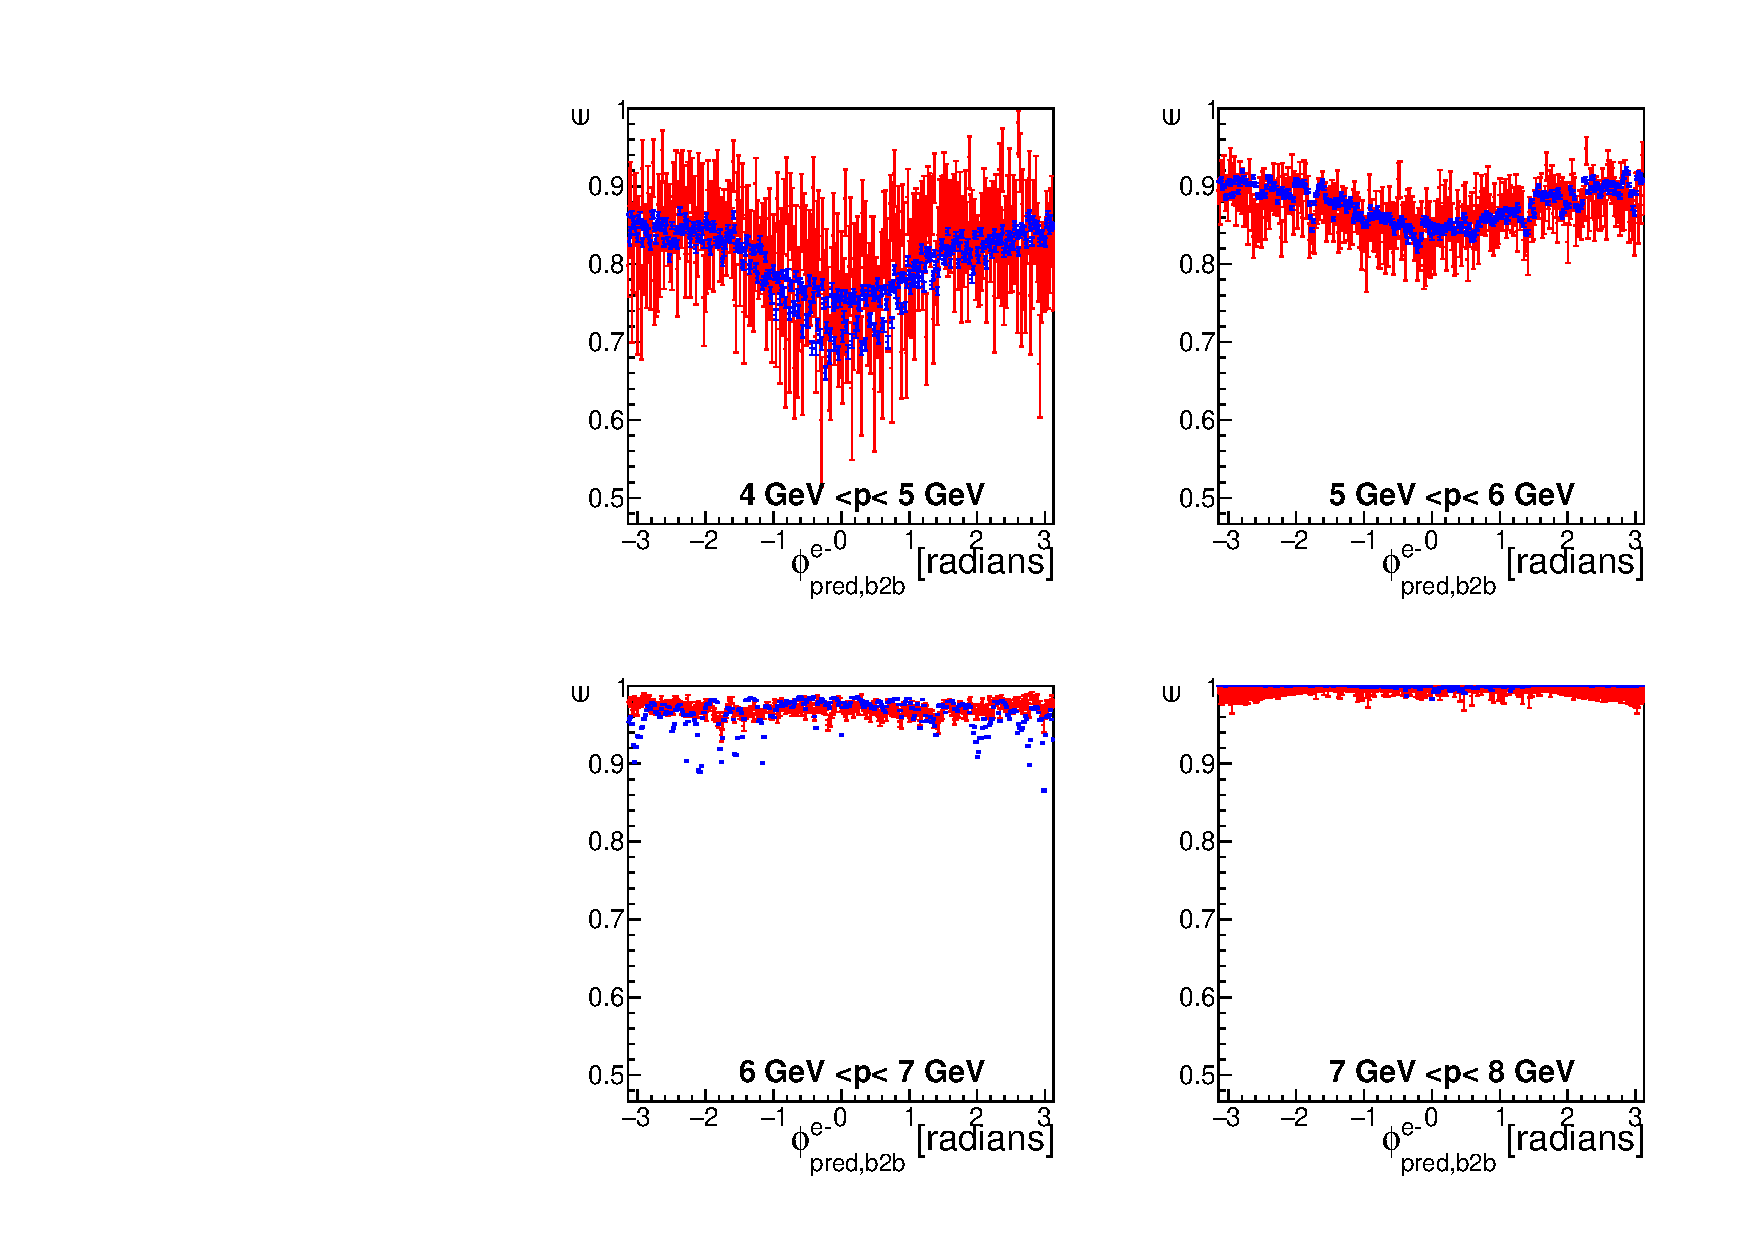
\includegraphics[width=\textwidth]{VPlots/P3/xPMPhiemFCP3}
	\end{textblock*}
	
	\begin{textblock*}{2cm}(2.3cm,-3.5cm)
		$\textrm{e}^-$
	\end{textblock*}
	
	\begin{textblock*}{2cm}(8.7cm,-3.5cm)
		$\textrm{e}^+$
	\end{textblock*}
	
	
	\begin{textblock*}{11cm}(5.5cm,-4.3cm)
		
		\begin{center}
			\line(0,1){256}
		\end{center}
		
	\end{textblock*}
	
	
	\begin{textblock*}{6.5cm}(6cm,-2.5cm)
		
		\setlength{\unitlength}{5cm}
		\begin{picture}(1,1)
		\put(0,0){\line(1,1){1}}
		
		\end{picture}
		
	\end{textblock*}
	
	
	
	\begin{textblock*}{4cm}(-0.5cm,-3.7cm)
		\textcolor{red}{Phase3 MC10}
		
		\textcolor{blue}{Phase3 Data}
	\end{textblock*}
	
	
		\pause[2]
	
	
	\begin{textblock*}{6cm}(5.6cm,-3.5cm)
		\begin{mybox}
			Electron Tracking Efficiency:
			\begin{itemize}
				\item<2-> Highest tracking efficiency for momenta between $7\,\textrm{GeV}$ and $8\,\textrm{GeV}$
				\item<3-> Minimum at $\phi_{\textrm{pred,b2b}} \approx 0$ for momenta between $4\,\textrm{GeV}$ and $6\,\textrm{GeV}$
				\item<4-> Weird \textit{ribbon} structure in the phase3 data tracking efficiency at $\phi_{\textrm{pred,b2b}} \approx 0$ for momenta between $4\,\textrm{GeV}$ and $5\,\textrm{GeV}$
				\item<5-> Weird efficiency drops in phase3 data for momenta between $6\,\textrm{GeV}$ and $7\,\textrm{GeV}$
			\end{itemize}
		\end{mybox}
	\end{textblock*}
	
	
	\begin{textblock*}{5cm}(0cm,-2.0cm)
		\begin{tikzpicture}
		\only<4>{
			\draw[line width=0.5mm,winered] \boundellipse{2cm,0cm}{.8cm}{.6cm};
		}
		\end{tikzpicture}
	\end{textblock*}
	
	
	\begin{textblock*}{5cm}(-0.6cm,0.3cm)
		\begin{tikzpicture}
		\only<5>{
			\draw[line width=0.5mm,winered] \boundellipse{2cm,0cm}{1.4cm}{.5cm};
		}
		\end{tikzpicture}
	\end{textblock*}
	
	\pause[6]
\end{frame}








\begin{frame}{Phase3 Tracking Efficiencies As Function Of $\phi_{\textrm{pred,b2b}}$; Barrel}
	
	
	\begin{textblock*}{6.5cm}(-0.9cm,-3cm)
		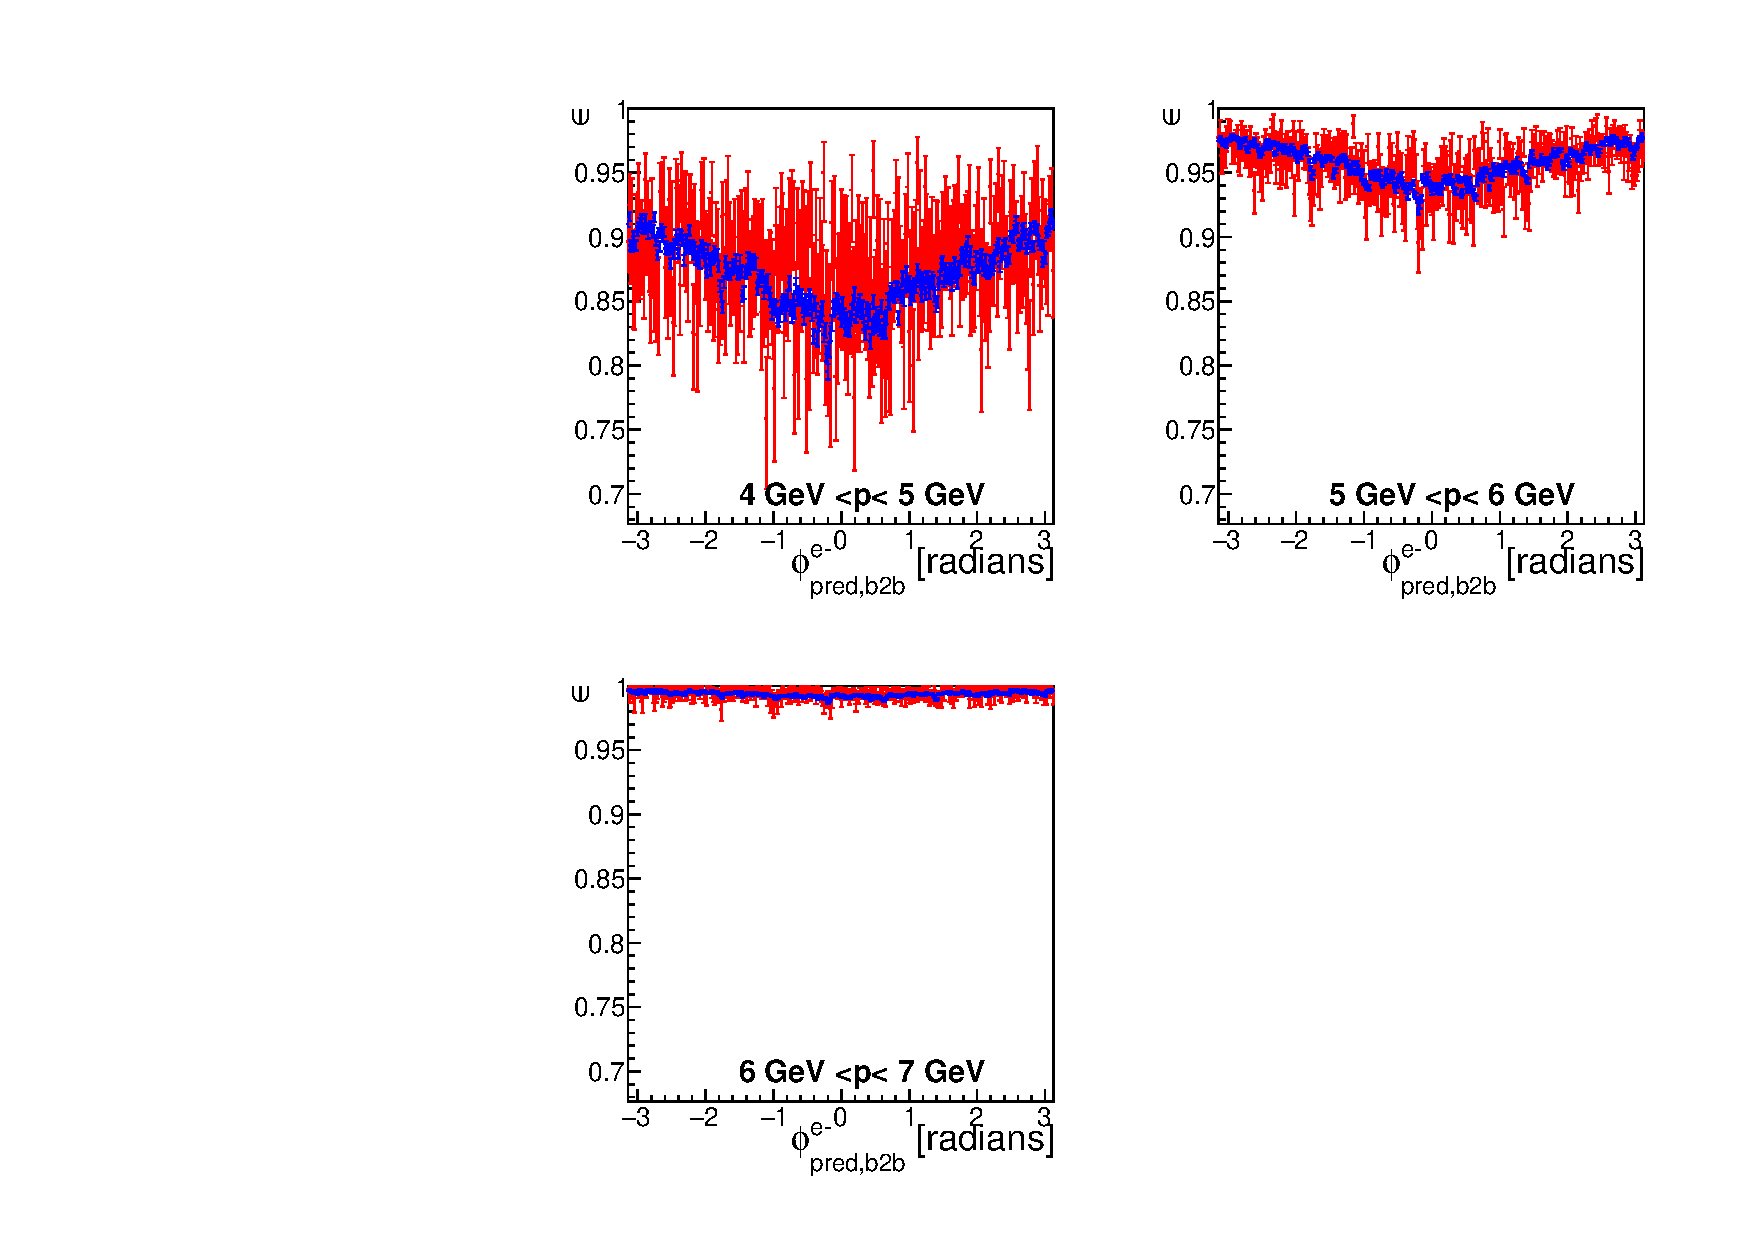
\includegraphics[width=\textwidth]{VPlots/P3/xPMPhiemBarrelP3}
	\end{textblock*}
	
	\begin{textblock*}{6.5cm}(5.5cm,-3cm)
		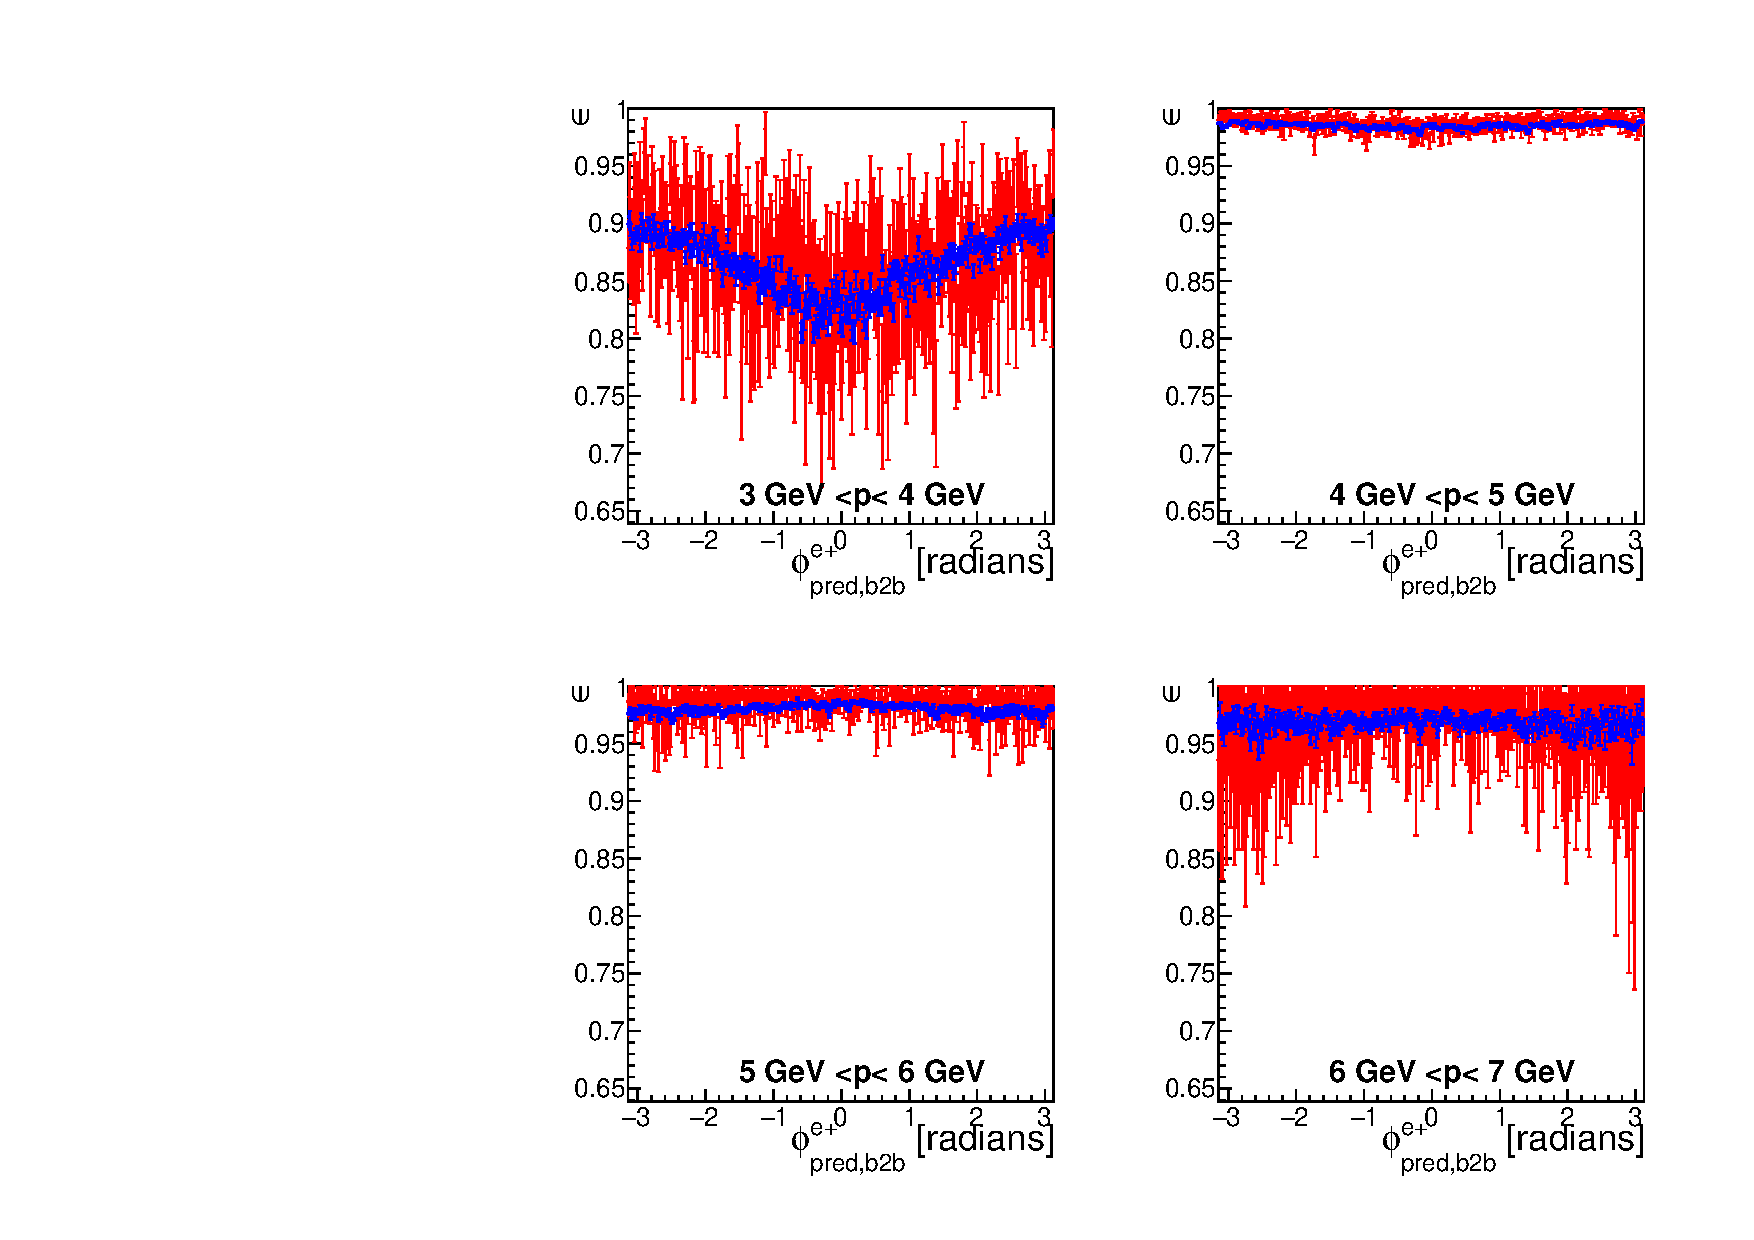
\includegraphics[width=\textwidth]{VPlots/P3/xPMPhiepBarrelP3}
	\end{textblock*}
	
	
	\begin{textblock*}{2cm}(2.3cm,-3.5cm)
		$\textrm{e}^-$
	\end{textblock*}
	
	\begin{textblock*}{2cm}(8.7cm,-3.5cm)
		$\textrm{e}^+$
	\end{textblock*}
	
	
	
	\begin{textblock*}{11cm}(5.5cm,-4.3cm)
		
		\begin{center}
			\line(0,1){256}
		\end{center}
		
	\end{textblock*}
	
	\only<1,2,3>{
	
	\begin{textblock*}{4cm}(-0.5cm,-3.7cm)
		\textcolor{red}{Phase3 MC10}
		
		\textcolor{blue}{Phase3 Data}
	\end{textblock*}
	
}
	
	
\only<4->{
	\begin{textblock*}{4cm}(6cm,-3.7cm)
	\textcolor{red}{Phase3 MC10}
	
	\textcolor{blue}{Phase3 Data}
\end{textblock*}


}
	
	
	
	\only<2,3>{
	
		\begin{textblock*}{6cm}(5.6cm,-3.5cm)
		\begin{mybox}
			Electron Tracking Efficiency:
			\begin{itemize}
				\item<2-> Highest tracking efficiency for momenta between $6\,\textrm{GeV}$ and $7\,\textrm{GeV}$
				\item<2-> Lowest tracking efficiency for momenta between $4\,\textrm{GeV}$ and $5\,\textrm{GeV}$
				
				\item<3-> Minimum at $\phi_{\textrm{pred,b2b}} \approx 0$ for momenta between $4\,\textrm{GeV}$ and $6\,\textrm{GeV}$
			\end{itemize}
		\end{mybox}
	\end{textblock*}
	}
	
	\pause[4]
	\begin{textblock*}{6cm}(-0.7cm,-3.5cm)
		\begin{mybox}
			Positron Tracking Efficiency:
			\begin{itemize}
				\item<2-> Highest tracking efficiency for momenta between $4\,\textrm{GeV}$ and $6\,\textrm{GeV}$
				\item<3-> Lowest tracking efficiency for momenta between $3\,\textrm{GeV}$ and $4\,\textrm{GeV}$
				\item<5-> Minimum at $\phi_{\textrm{pred,b2b}} \approx 0$ for momenta between $3\,\textrm{GeV}$ and $4\,\textrm{GeV}$
			\end{itemize}
		\end{mybox}
	\end{textblock*}
	
	
	
	
	
	
\end{frame}



\begin{frame}{Phase3 Tracking Efficiencies As Function Of $\phi_{\textrm{pred,b2b}}$; Backward End-Cap}
	
	
	\begin{textblock*}{6.5cm}(5.5cm,-3cm)
		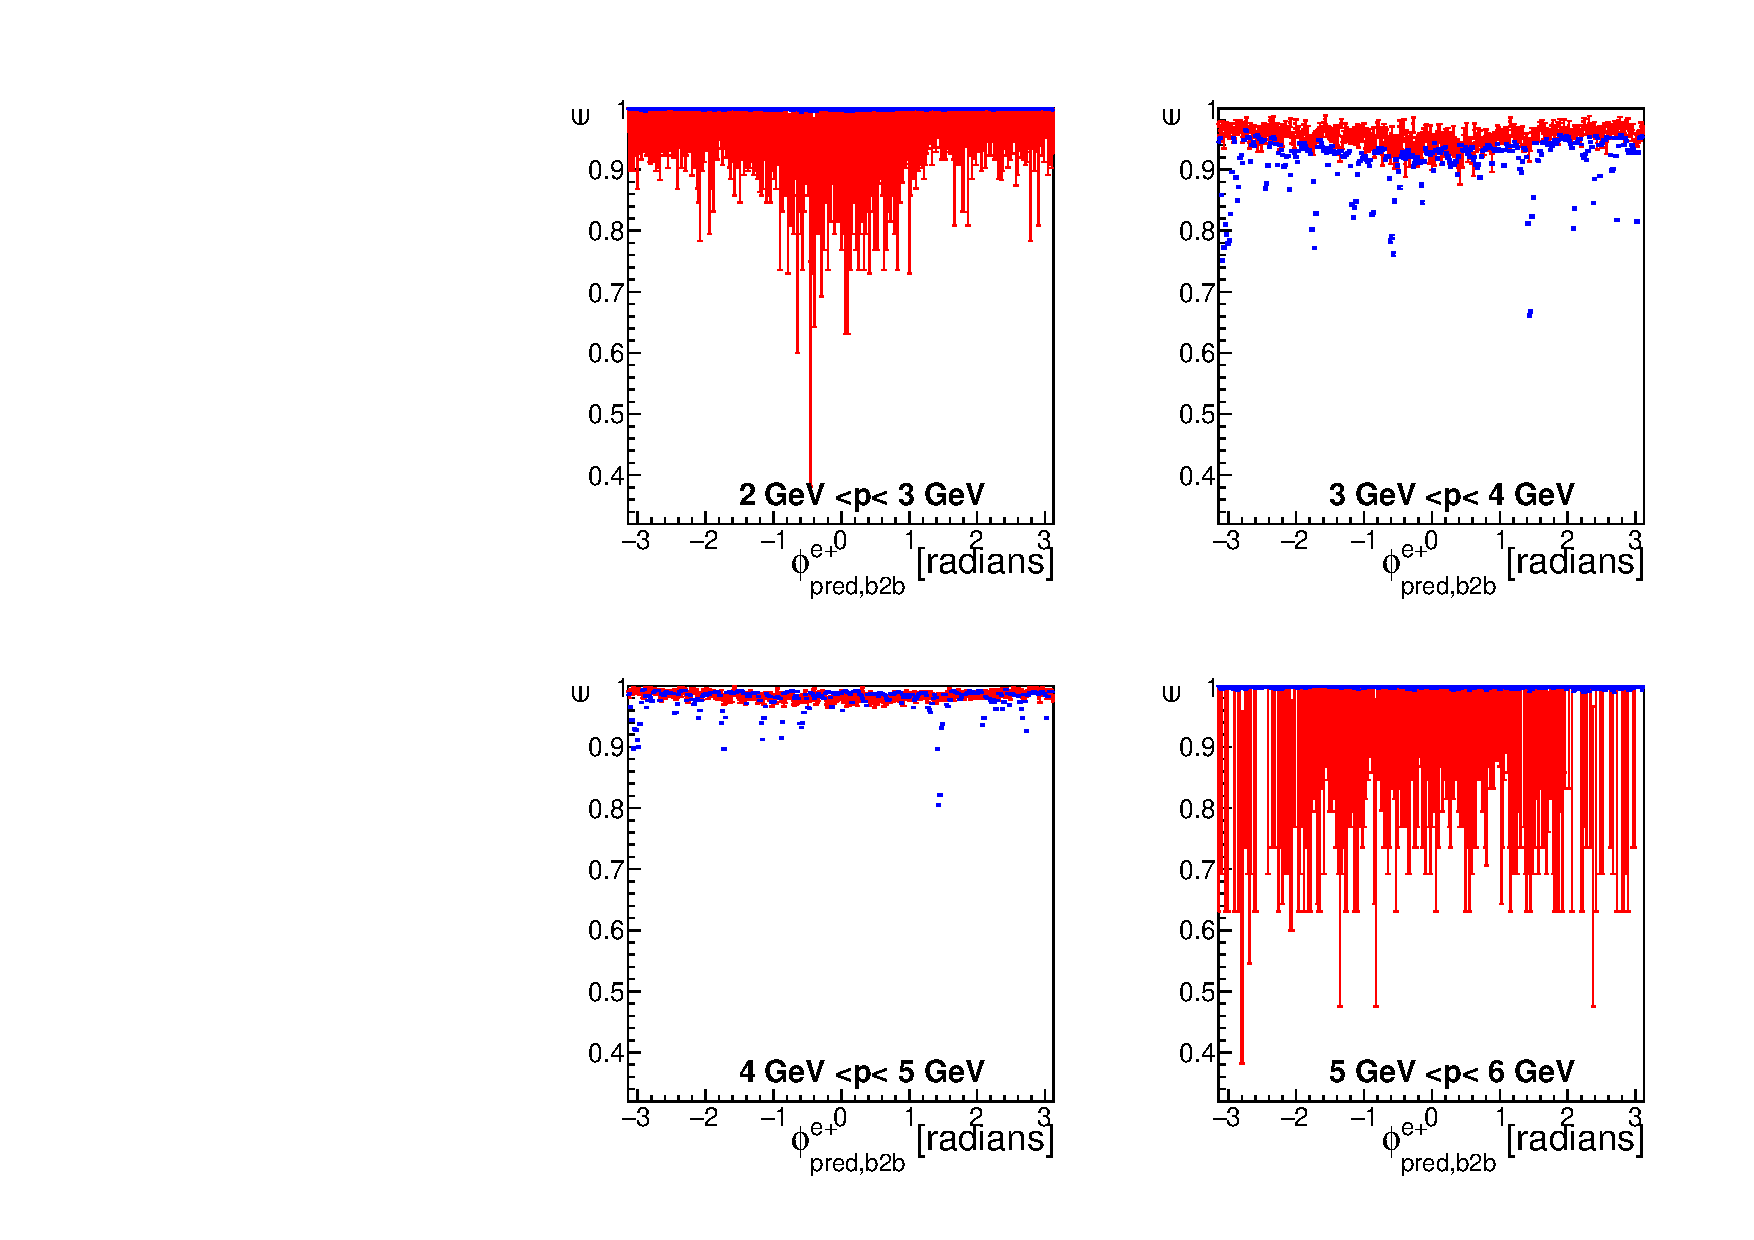
\includegraphics[width=\textwidth]{VPlots/P3/xPMPhiepECP3}
	\end{textblock*}
	
	\begin{textblock*}{2cm}(2.3cm,-3.5cm)
		$\textrm{e}^-$
	\end{textblock*}
	
	\begin{textblock*}{2cm}(8.7cm,-3.5cm)
		$\textrm{e}^+$
	\end{textblock*}
	
	
	\begin{textblock*}{11cm}(5.5cm,-4.3cm)
		
		\begin{center}
			\line(0,1){256}
		\end{center}
		
	\end{textblock*}
	
	
	\begin{textblock*}{6.5cm}(-0.2cm,-2.5cm)
		
		\setlength{\unitlength}{5cm}
		\begin{picture}(1,1)
		\put(0,0){\line(1,1){1}}
		
		\end{picture}
		
	\end{textblock*}
	
	
	
	\only<1>{
	
	\begin{textblock*}{4cm}(-0.5cm,-3.7cm)
		\textcolor{red}{Phase3 MC10}
		
		\textcolor{blue}{Phase3 Data}
	\end{textblock*}
	}
		\only<2->{
		
		\begin{textblock*}{4cm}(6cm,-3.7cm)
			\textcolor{red}{Phase3 MC10}
			
			\textcolor{blue}{Phase3 Data}
		\end{textblock*}
	}
	
	
	
	
		\begin{textblock*}{6cm}(-0.7cm,-3.5cm)
		\only<2->{
			\begin{mybox}
				Positron Tracking Efficiency:
				\begin{itemize}
					
					\item The highest phase3 data tracking efficiency occurs for momenta between $2\,\textrm{GeV}$ and $3\,\textrm{GeV}$ and $5\,\textrm{GeV}$ and $6\,\textrm{GeV}$
					\item<3-> Weird efficiency drops in the phase3 data tracking efficiency for momenta between $3\,\textrm{GeV}$ and $5\,\textrm{GeV}$

				\end{itemize}
			\end{mybox}
		}
	\end{textblock*}
	
	
	
		\begin{textblock*}{5cm}(5.8cm,0.2cm)
		\begin{tikzpicture}
		\only<3>{
			\draw[line width=0.5mm,winered] \boundellipse{2cm,0cm}{1.4cm}{.6cm};
		}
		\end{tikzpicture}
	\end{textblock*}
	
	
			\begin{textblock*}{5cm}(9cm,-2.9cm)
		\begin{tikzpicture}
		\only<3>{
			\draw[line width=0.5mm,winered] \boundellipse{2cm,0cm}{1.4cm}{.8cm};
		}
		\end{tikzpicture}
	\end{textblock*}
	
	\pause[4]
	
	
	
\end{frame}




\section{Comparing The Tracking Efficiency Of Phase2 Data with Phase3 Data}






\begin{frame}{Tracking Efficiencies As Function Of $\theta_{\textrm{pred,b2b}}$}



\begin{textblock*}{6.5cm}(-0.9cm,-3cm)
		
	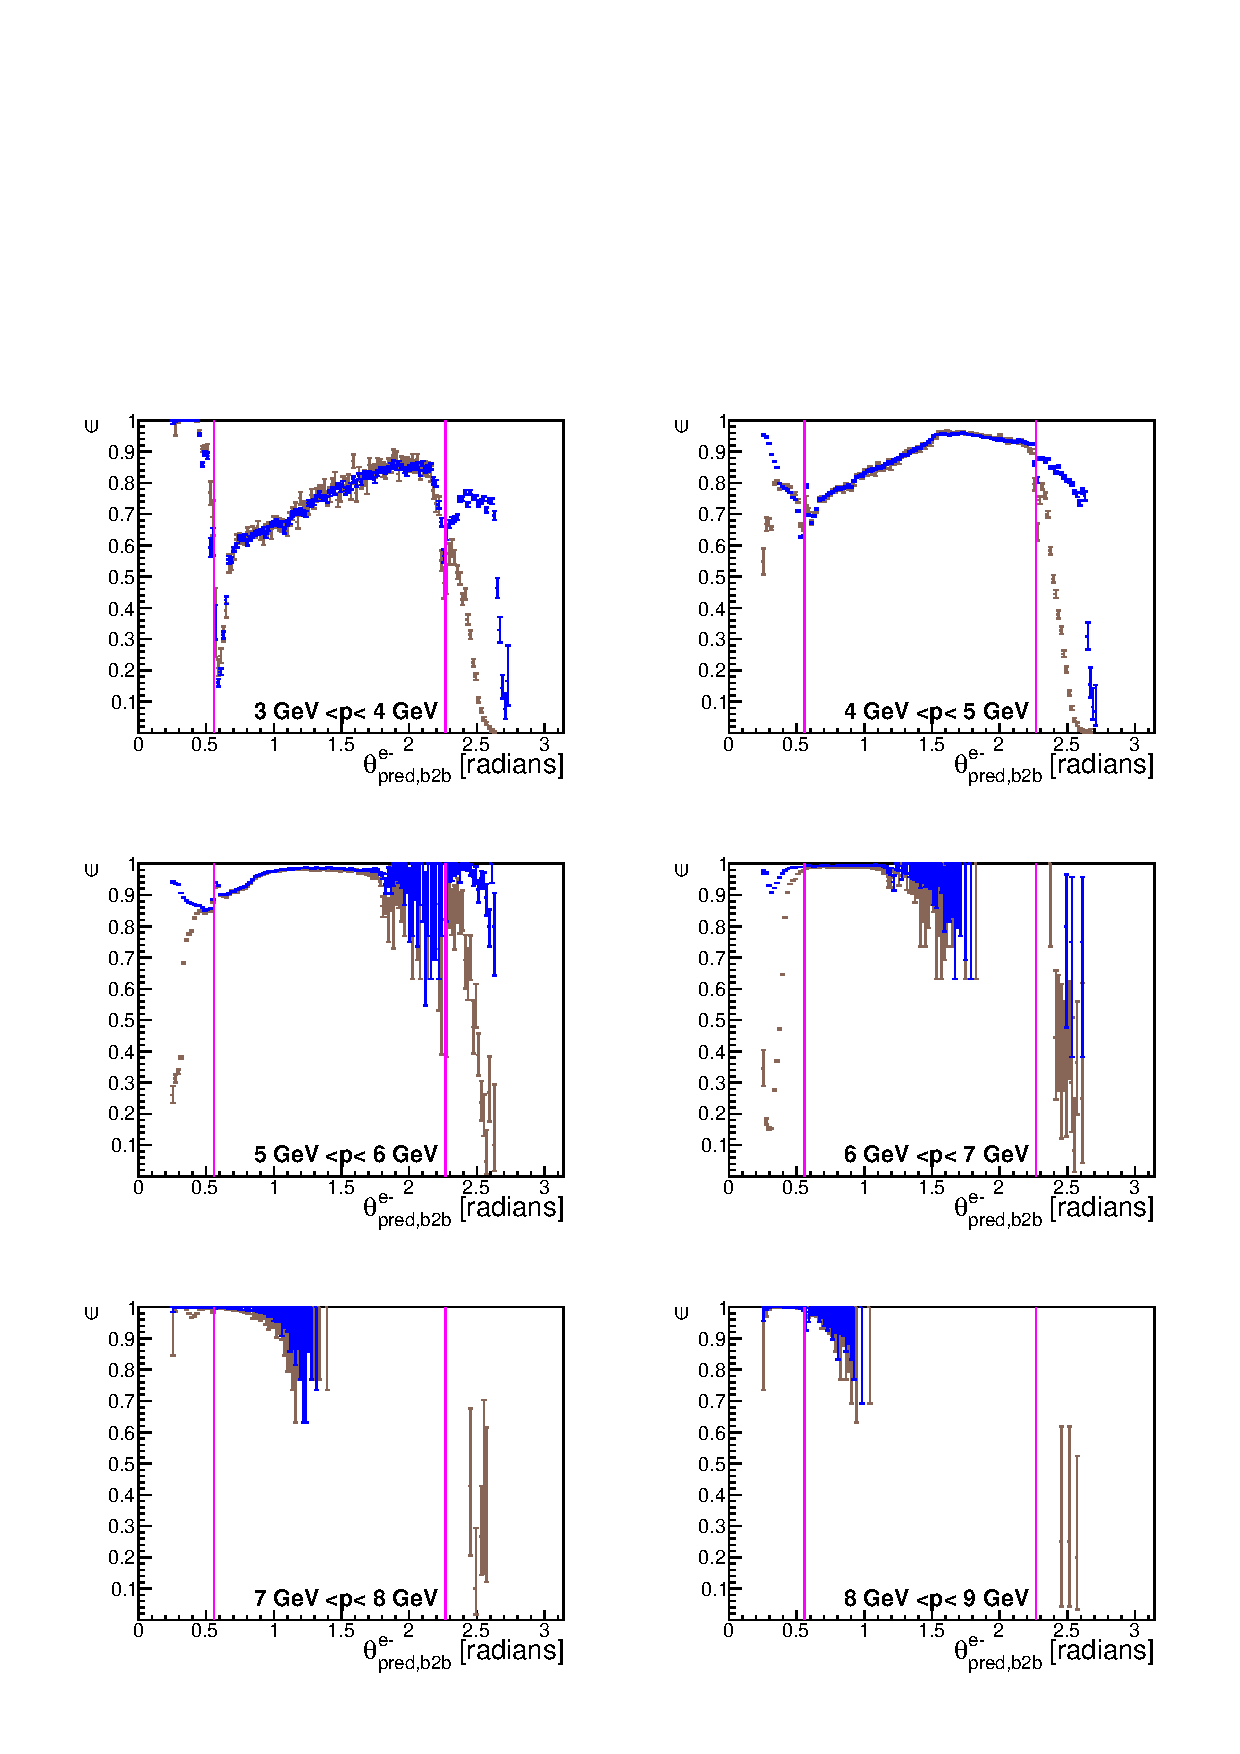
\includegraphics[width=\textwidth]{VPlots/Comp/cMThetaem_Data}
\end{textblock*}

\begin{textblock*}{6.5cm}(5.5cm,-3cm)
	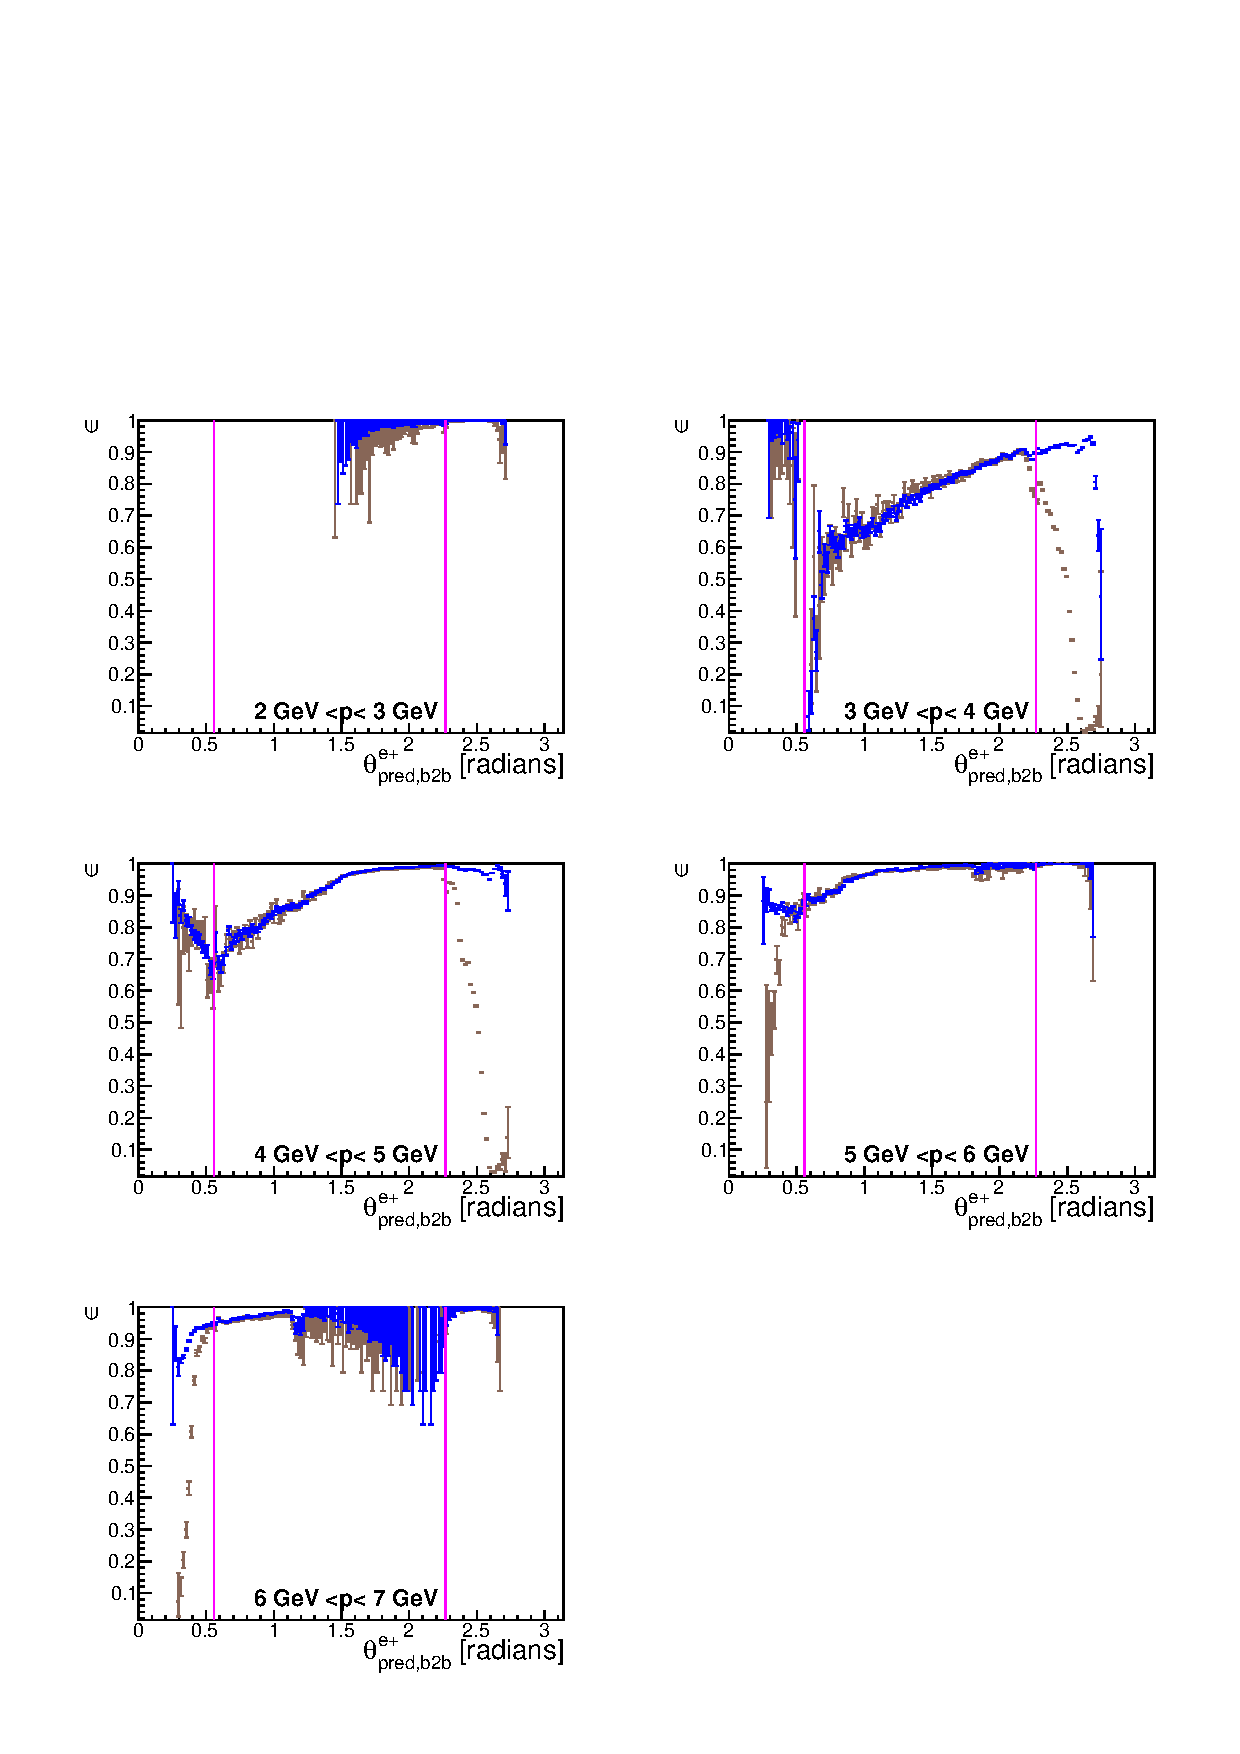
\includegraphics[width=\textwidth]{VPlots/Comp/cMThetaep_Data}
\end{textblock*}


\begin{textblock*}{2cm}(2.3cm,-3.5cm)
	$\textrm{e}^-$
\end{textblock*}

\begin{textblock*}{2cm}(8.7cm,-3.5cm)
	$\textrm{e}^+$
\end{textblock*}



\begin{textblock*}{11cm}(5.5cm,-4.3cm)
	
	\begin{center}
		\line(0,1){256}
	\end{center}
	
\end{textblock*}

\only<1,2,3,4>{
\begin{textblock*}{4cm}(-0.5cm,-3.7cm)
	\textcolor{brown}{Phase2 Data}
	
	\textcolor{blue}{Phase3 Data}
\end{textblock*}
}

\only<5->{
	\begin{textblock*}{4cm}(6cm,-3.7cm)
		\textcolor{brown}{Phase2 Data}
		
		\textcolor{blue}{Phase3 Data}
	\end{textblock*}
}






		\only<2,3,4>{
	\begin{textblock*}{6cm}(5.6cm,-3.5cm)
		\begin{mybox}
			Electron Tracking Efficiency:
			\begin{itemize}
				\item<2-> Drastic improvement in the end-caps
				\item<4> Tracking efficiency in the barrel stayed more or less the same
				
			\end{itemize}
		\end{mybox}
	\end{textblock*}
}






\begin{textblock*}{5cm}(1.2cm,-2.8cm)
	\begin{tikzpicture}
	\only<3>{
		\draw[line width=0.5mm,winered] \boundellipse{2cm,0cm}{0.3cm}{1.cm};
	}
	\end{tikzpicture}
\end{textblock*}

\begin{textblock*}{5cm}(2.8cm,-2.8cm)
	\begin{tikzpicture}
	\only<3>{
		\draw[line width=0.5mm,winered] \boundellipse{2cm,0cm}{0.3cm}{1.cm};
	}
	\end{tikzpicture}
\end{textblock*}


\begin{textblock*}{5cm}(4.4cm,-2.8cm)
	\begin{tikzpicture}
	\only<3>{
		\draw[line width=0.5mm,winered] \boundellipse{2cm,0cm}{0.3cm}{1.cm};
	}
	\end{tikzpicture}
\end{textblock*}


\begin{textblock*}{5cm}(-0.5cm,-0.4cm)
	\begin{tikzpicture}
	\only<3>{
		\draw[line width=0.5mm,winered] \boundellipse{2cm,0cm}{0.3cm}{1.cm};
	}
	\end{tikzpicture}
\end{textblock*}


\begin{textblock*}{5cm}(1.2cm,-0.4cm)
	\begin{tikzpicture}
	\only<3>{
		\draw[line width=0.5mm,winered] \boundellipse{2cm,0cm}{0.3cm}{1.cm};
	}
	\end{tikzpicture}
\end{textblock*}

\begin{textblock*}{5cm}(2.8cm,-0.4cm)
	\begin{tikzpicture}
	\only<3>{
		\draw[line width=0.5mm,winered] \boundellipse{2cm,0cm}{0.3cm}{1.cm};
	}
	\end{tikzpicture}
\end{textblock*}



		\begin{textblock*}{6cm}(-0.7cm,-3.5cm)
	
	\only<5,6,7>{
		\begin{mybox}
			Positron Tracking Efficiency:
			\begin{itemize}
				
				\item<5-> Drastic improvement in the end-caps
				\item<7-> Tracking efficiency in the barrel stayed more or less the same
				
			\end{itemize}
		\end{mybox}
	}
\end{textblock*}



\begin{textblock*}{5cm}(9.2cm,-0.4cm)
	\begin{tikzpicture}
	\only<6>{
		\draw[line width=0.5mm,winered] \boundellipse{2cm,0cm}{0.3cm}{1.cm};
	}
	\end{tikzpicture}
\end{textblock*}


\begin{textblock*}{5cm}(10.85cm,-2.8cm)
	\begin{tikzpicture}
	\only<6>{
		\draw[line width=0.5mm,winered] \boundellipse{2cm,0cm}{0.3cm}{1.cm};
	}
	\end{tikzpicture}
\end{textblock*}

\begin{textblock*}{5cm}(7.6cm,-0.4cm)
	\begin{tikzpicture}
	\only<6>{
		\draw[line width=0.5mm,winered] \boundellipse{2cm,0cm}{0.3cm}{1.cm};
	}
	\end{tikzpicture}
\end{textblock*}




\begin{textblock*}{5cm}(6.cm,2.cm)
	\begin{tikzpicture}
	\only<6>{
		\draw[line width=0.5mm,winered] \boundellipse{2cm,0cm}{0.3cm}{1.cm};
	}
	\end{tikzpicture}
\end{textblock*}




\begin{textblock*}{8cm}(1.5cm,-.8cm)
	\only<8>{
		
		\begin{mybox}
			We will only compare the tracking efficiencies for electrons in the forward end-cap and the tracking efficiencies for positrons in the backward end-cap
		\end{mybox}
		
	}
	
\end{textblock*}





\end{frame}


\begin{frame}{Tracking Efficiencies As Function Of $\phi_{\textrm{pred,b2b}}$; Forward End-Cap}
	
	
	\begin{textblock*}{6.5cm}(-0.9cm,-3cm)
		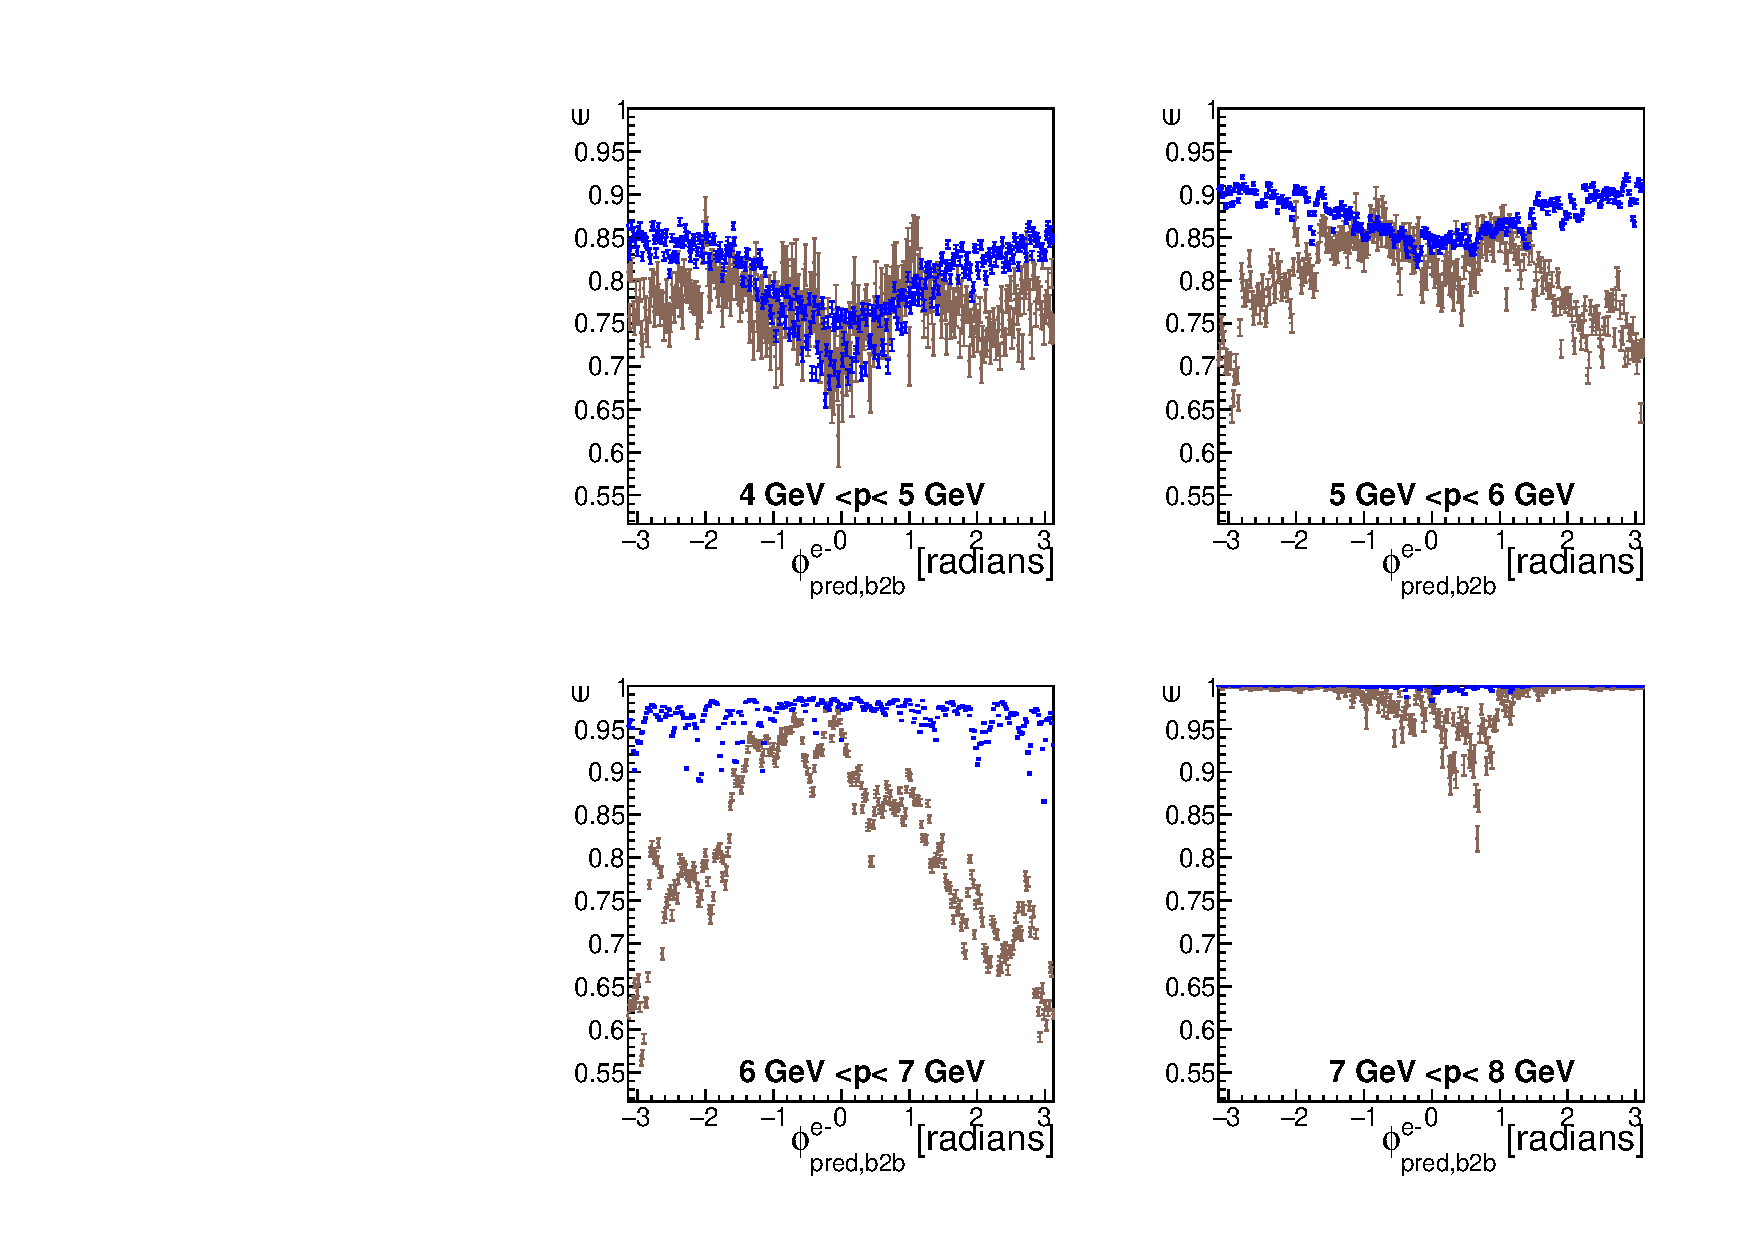
\includegraphics[width=\textwidth]{VPlots/Comp/cMPhiemFC_Data}
	\end{textblock*}
	
	\begin{textblock*}{2cm}(2.3cm,-3.5cm)
		$\textrm{e}^-$
	\end{textblock*}
	
%	\begin{textblock*}{2cm}(8.7cm,-3.5cm)
%		$\textrm{e}^+$
%	\end{textblock*}
	
	
	\begin{textblock*}{11cm}(5.5cm,-4.3cm)
		
		\begin{center}
			\line(0,1){256}
		\end{center}
		
	\end{textblock*}
	
	
	\begin{textblock*}{6.5cm}(6cm,-2.5cm)
		
		\setlength{\unitlength}{5cm}
		\begin{picture}(1,1)
%		\put(0,0){\line(1,1){1}}
		
		\end{picture}
		
	\end{textblock*}
	
	
	
	\begin{textblock*}{4cm}(-0.5cm,-3.7cm)
		\textcolor{brown}{Phase2 Data}
		
		\textcolor{blue}{Phase3 Data}
	\end{textblock*}
	
	
	\begin{textblock*}{6cm}(5.6cm,-3.5cm)
		\begin{mybox}
			Electron Tracking Efficiency:
			\begin{itemize}
				\item The tracking efficiency improved over almost all $\phi_{\textrm{pred,b2b}}$ (exception occurs for $\phi_{\textrm{pred,b2b}} \approx 1$ for momenta between $4\,\textrm{GeV}$ and $5\,\textrm{GeV}$)
				
				\item<3-> The tracking efficiency improved drastically for momenta between $6\,\textrm{GeV}$ and $7\,\textrm{GeV}$
				\item<4-> No efficiency drops for momenta between $7\,\textrm{GeV}$ and $8\,\textrm{GeV}$ in the phase3 data tracking efficiency
			\end{itemize}
		\end{mybox}
	\end{textblock*}
	
		
	\begin{textblock*}{5cm}(0.7cm,-2.1cm)
		\begin{tikzpicture}
		\only<2>{
			\draw[line width=0.5mm,winered] \boundellipse{2cm,0cm}{0.4cm}{0.3cm};
		}
		\end{tikzpicture}
	\end{textblock*}	
	
	
	
	
		\begin{textblock*}{5cm}(-0.7cm,.10cm)
		\begin{tikzpicture}
		\only<3>{
			\draw[line width=0.5mm,winered] \boundellipse{2cm,0cm}{1.5cm}{1.5cm};
		}
		\end{tikzpicture}
	\end{textblock*}
	
	
\begin{textblock*}{5cm}(-0.7cm,.10cm)
	\begin{tikzpicture}
	\only<3>{
		\draw[line width=0.5mm,winered] \boundellipse{2cm,0cm}{1.5cm}{1.5cm};
	}
	\end{tikzpicture}
\end{textblock*}	
	
	
		
	\begin{textblock*}{5cm}(3.1cm,.30cm)
		\begin{tikzpicture}
		\only<4>{
			\draw[line width=0.5mm,winered] \boundellipse{3cm,0cm}{1.cm}{.6cm};
		}
		\end{tikzpicture}
	\end{textblock*}
	
	
	
	

	\pause[5]
	
\end{frame}

\begin{frame}{Tracking Efficiencies As Function Of $\phi_{\textrm{pred,b2b}}$; Backward End-Cap}
	
	
	\begin{textblock*}{6.5cm}(5.5cm,-3cm)
		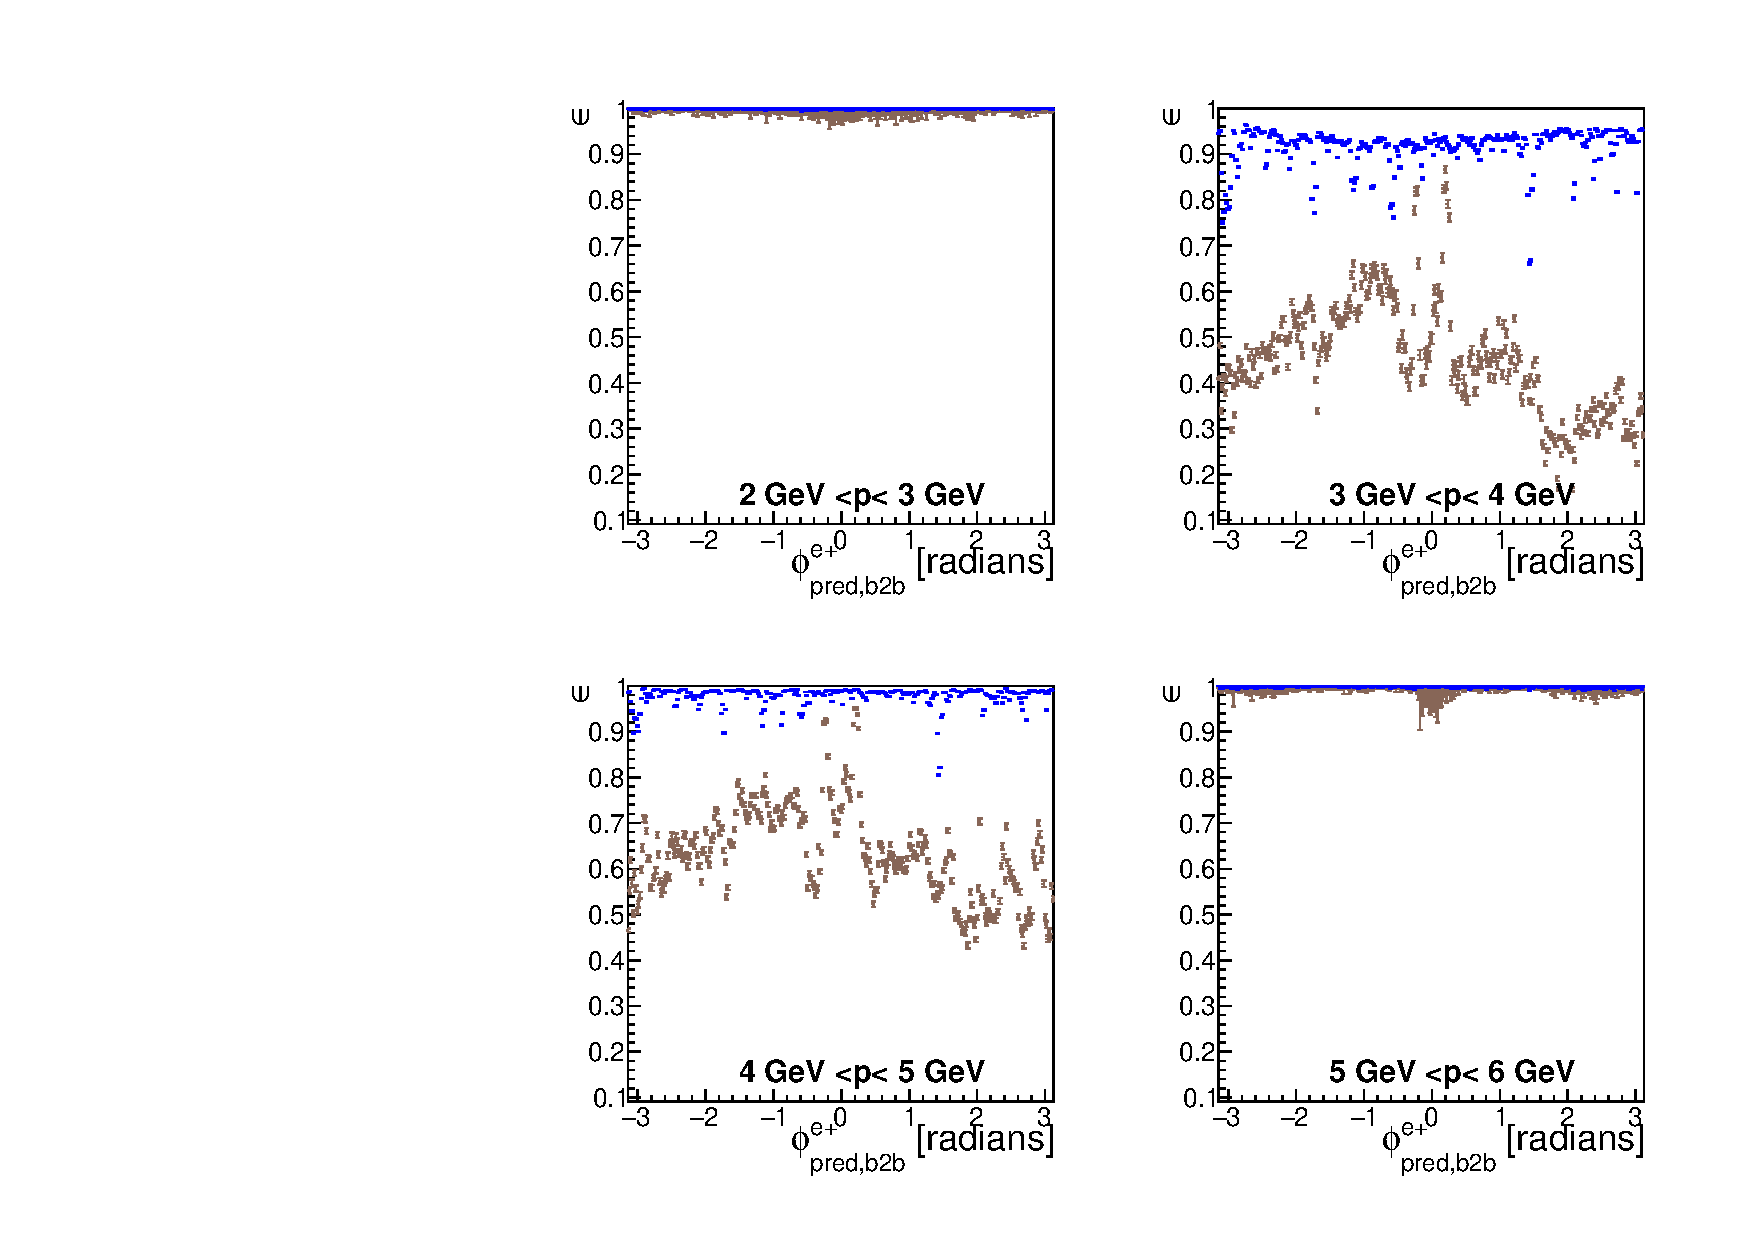
\includegraphics[width=\textwidth]{VPlots/Comp/cMPhiepEC_Data}
	\end{textblock*}
	
	\begin{textblock*}{2cm}(2.3cm,-3.5cm)
%		$\textrm{e}^-$
	\end{textblock*}
	
	\begin{textblock*}{2cm}(8.7cm,-3.5cm)
		$\textrm{e}^+$
	\end{textblock*}
	
	
	\begin{textblock*}{11cm}(5.5cm,-4.3cm)
		
		\begin{center}
			\line(0,1){256}
		\end{center}
		
	\end{textblock*}
	
	
	\begin{textblock*}{6.5cm}(-0.2cm,-2.5cm)
		
		\setlength{\unitlength}{5cm}
		\begin{picture}(1,1)
%		\put(0,0){\line(1,1){1}}
		
		\end{picture}
		
	\end{textblock*}
	
	\begin{textblock*}{4cm}(6cm,-3.7cm)
		\textcolor{brown}{Phase2 Data}
		
		\textcolor{blue}{Phase3 Data}
	\end{textblock*}
	
	
	
	\begin{textblock*}{6cm}(-0.7cm,-3.5cm)
		
		
			\begin{mybox}
				Positron Tracking Efficiency:
				\begin{itemize}					
					\item The tracking efficiencies for momenta between $2\,\textrm{GeV}$ and $3\,\textrm{GeV}$ and between $5\,\textrm{GeV}$ and $6\,\textrm{GeV}$ look very similar
					
					\item<2,3> The tracking efficiency for momenta between $3\,\textrm{GeV}$ and $5\,\textrm{GeV}$ improved drastically 
				\end{itemize}
			\end{mybox}
		
	\end{textblock*}
	
	
	
			\begin{textblock*}{5cm}(5.7cm,.10cm)
		\begin{tikzpicture}
		\only<2>{
			\draw[line width=0.5mm,winered] \boundellipse{2cm,0cm}{1.5cm}{1.5cm};
		}
		\end{tikzpicture}
	\end{textblock*}
	
	
	
	\begin{textblock*}{5cm}(8.95cm,-3.1cm)
		\begin{tikzpicture}
		\only<2>{
			\draw[line width=0.5mm,winered] \boundellipse{2cm,0cm}{1.5cm}{1.5cm};
		}
		\end{tikzpicture}
	\end{textblock*}
	
	
	
	
	
	\pause[3]
	
	
	
	
	
	
\end{frame}



\section{Conclusion}

\begin{frame}{Conclusion}
	
	
	\begin{itemize}
		\item It is possible to select Bhabha events using only information coming from the ECL
		\item The phase3 MC tracking efficiency is very close to the phase3 data tracking efficiency
		
		\item On phase3 data \textit{random} efficiency drops appear for some momenta in the end-caps 
		\item Drastic improvement in the tracking efficiency in the end-caps for phase3 compared to phase2
	\end{itemize}
	
	
	
	
\end{frame}

%--------------------------------------------


\appendix
\section{Appendix}
\begin{frame}{Code}


\lstset{language=Python}
\lstset{label={lst:code_direct}}
\lstset{basicstyle=\normalsize}

\begin{textblock*}{\textwidth}(-0cm,-3.7cm)
	
	\lstinputlisting[language=Python]{mesh.py}
	
	
\end{textblock*}


\end{frame}

\begin{frame}{More Events}
	
	\begin{textblock*}{10cm}(0cm,-3.7cm)
		
		Phase2 data:
		\begin{itemize}
			\item /ghi/fs01/belle2/bdata//Data/release-03-00-03/
			DB00000528/proc00000008/e0003/4S/r0*/all/mdst/sub00/*.root
			\item proc9
		\end{itemize}
		Phase2 MC:
		
		\begin{itemize}
			\item /belle/MC/release-01-00-02/DB00000294/MC10/ prod00004668/s00/e1002/4S/r00000/3600520000/mdst/sub00
		\end{itemize}
		
		
		Phase3 data:
		\begin{itemize}
			\item Exp7: /group/belle2/dataprod/Data/release-03-02-02/DB00000654/proc9/e0007/4S/r0*/all/mdst/sub00/*.root
			\item Exp8: /group/belle2/dataprod/Data/release-03-02-02/DB00000654/proc9/e0008/4S/r0*/all/mdst/sub00/*.root
			
			\item proc9
		\end{itemize}
		
		Phase3 MC:
		
		\begin{itemize}
			\item /belle/MC/release-01-00-02/DB00000294/MC10/ prod00004664/s00/e0000/4S/r00000/3600520000/mdst/sub00
		\end{itemize}
		
		
		
		
		
		
	\end{textblock*}
	
	
	
	
	
	
\end{frame}


\begin{frame}
	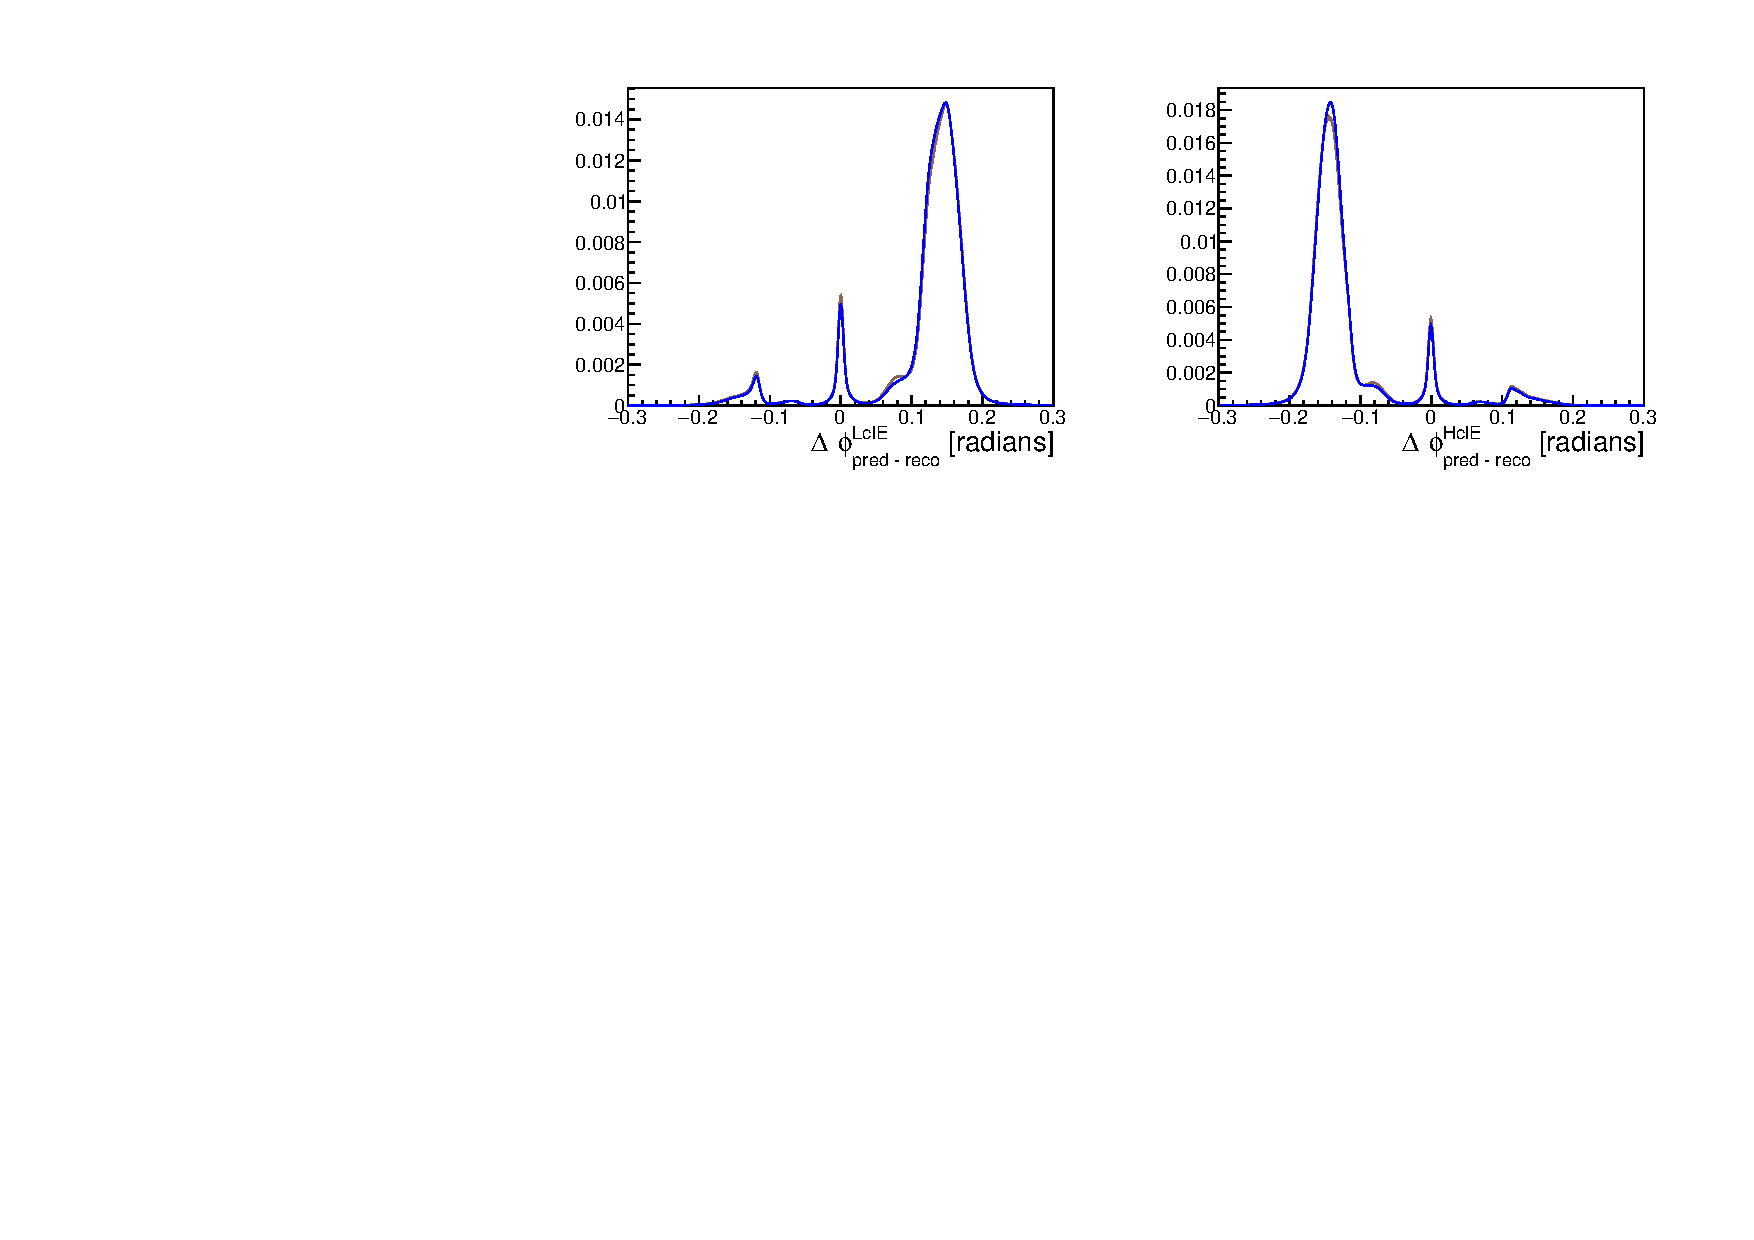
\includegraphics[width=\textwidth]{VBilder/cb2b}

	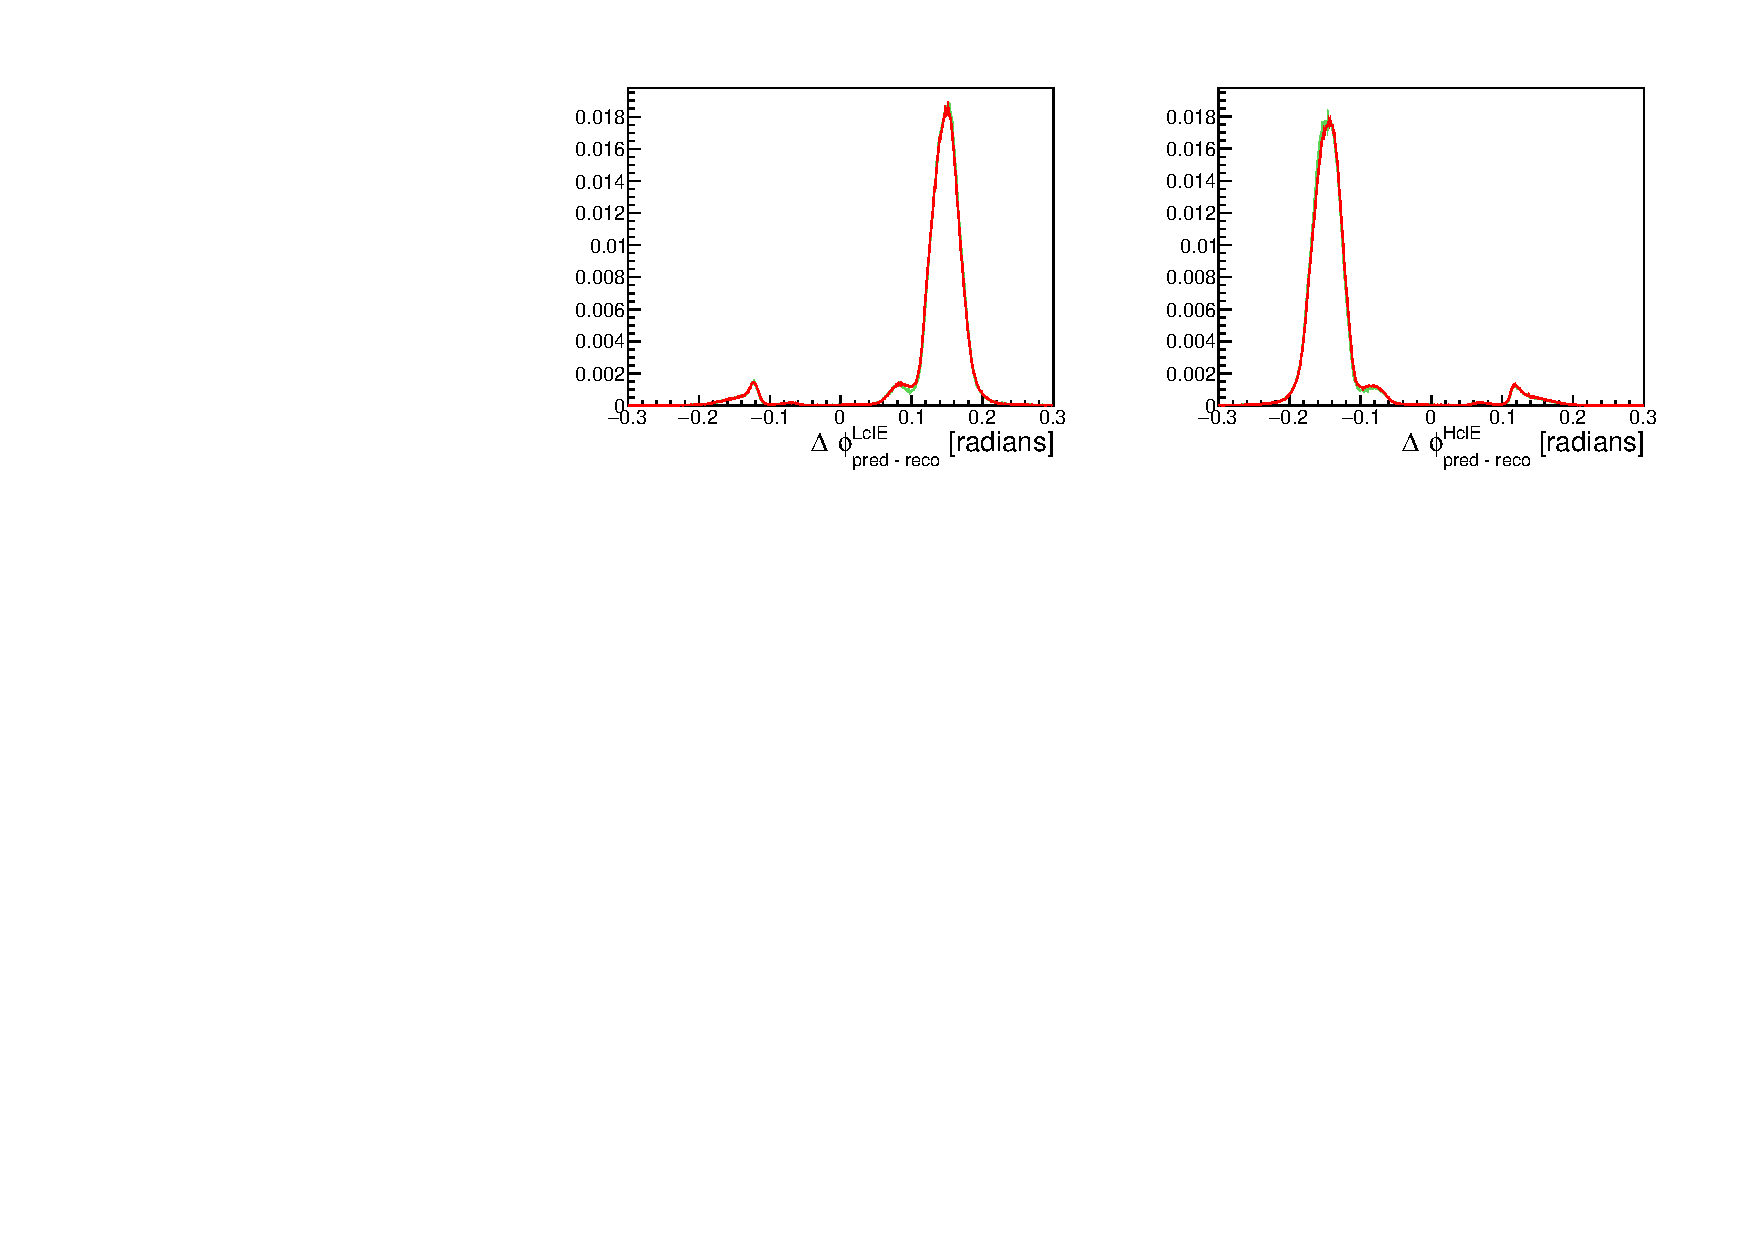
\includegraphics[width=\textwidth]{VBilder/cb2bMC}
\end{frame}


\begin{frame}
	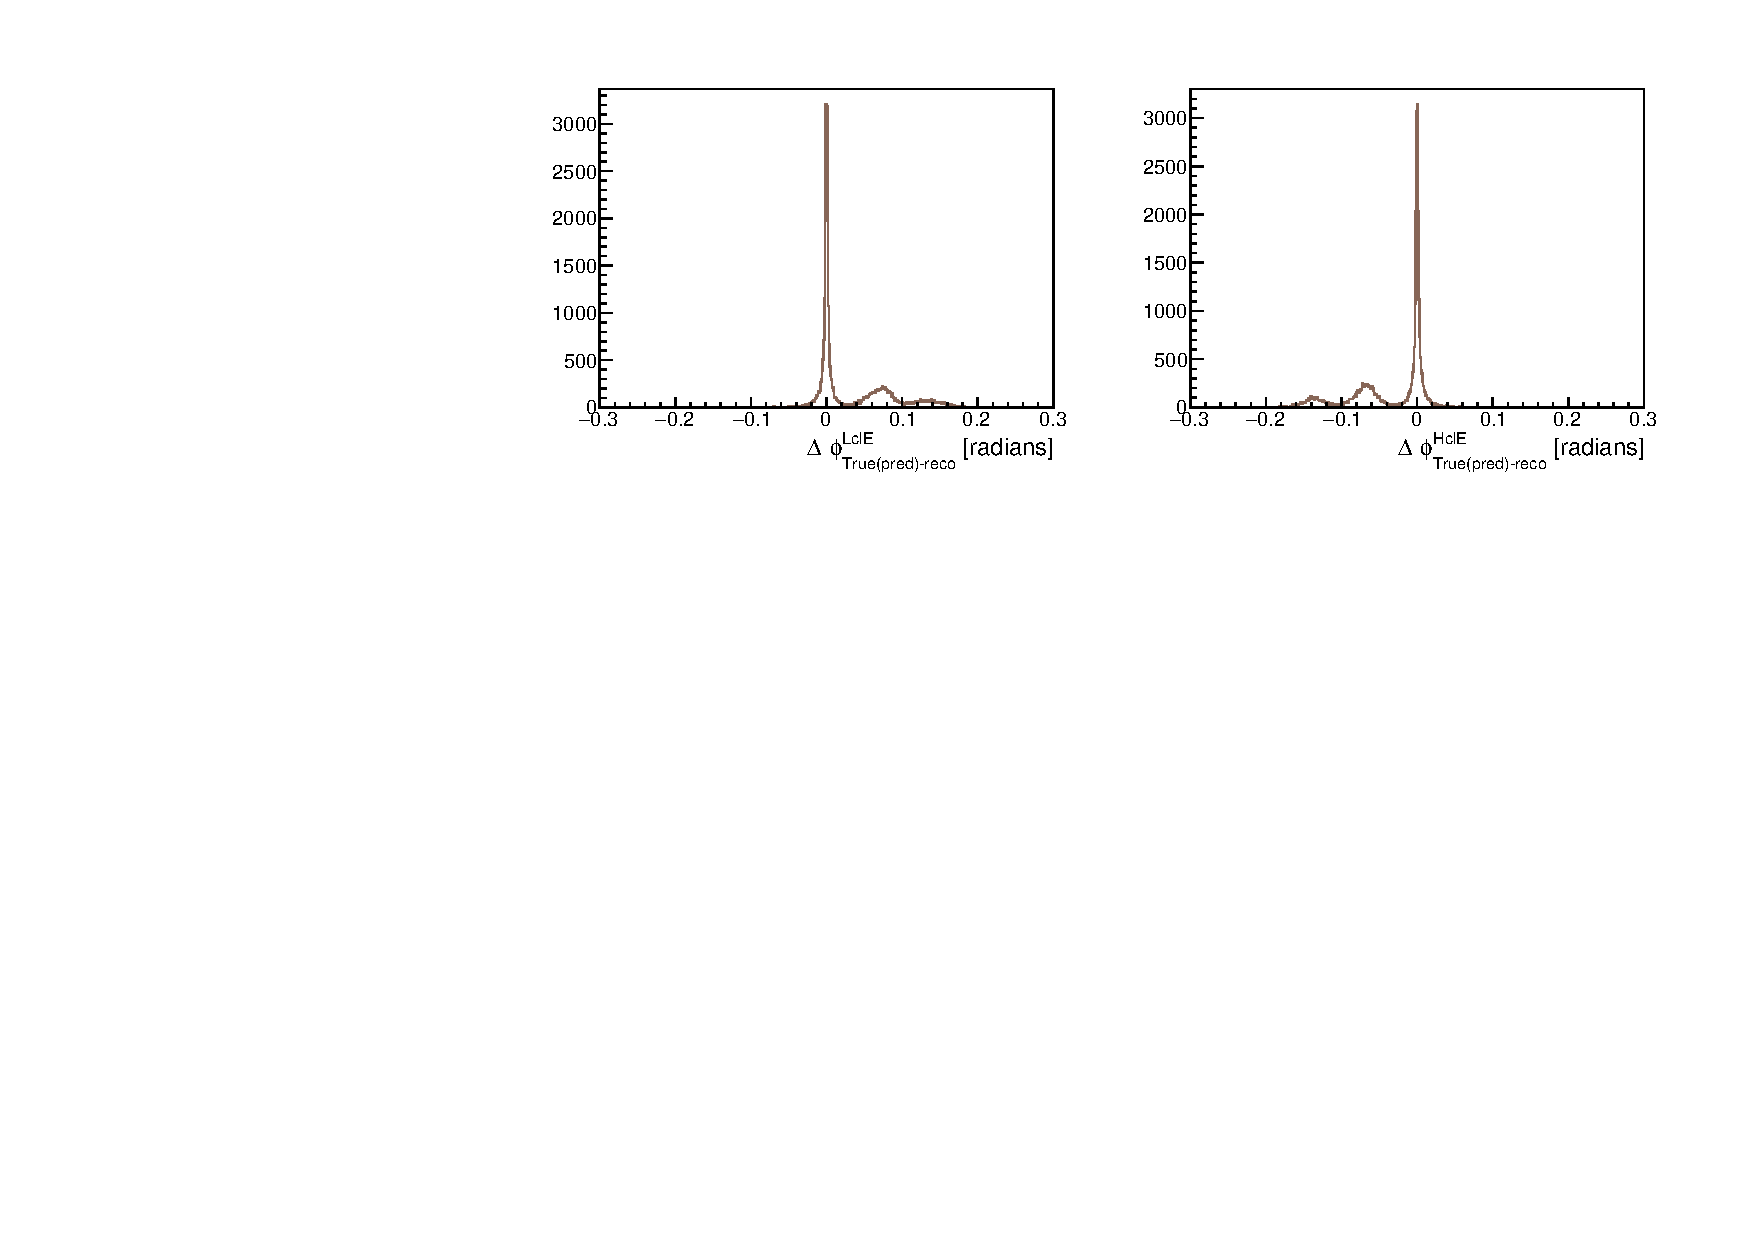
\includegraphics[width=\textwidth]{VBilder/b2b_Data}
	
	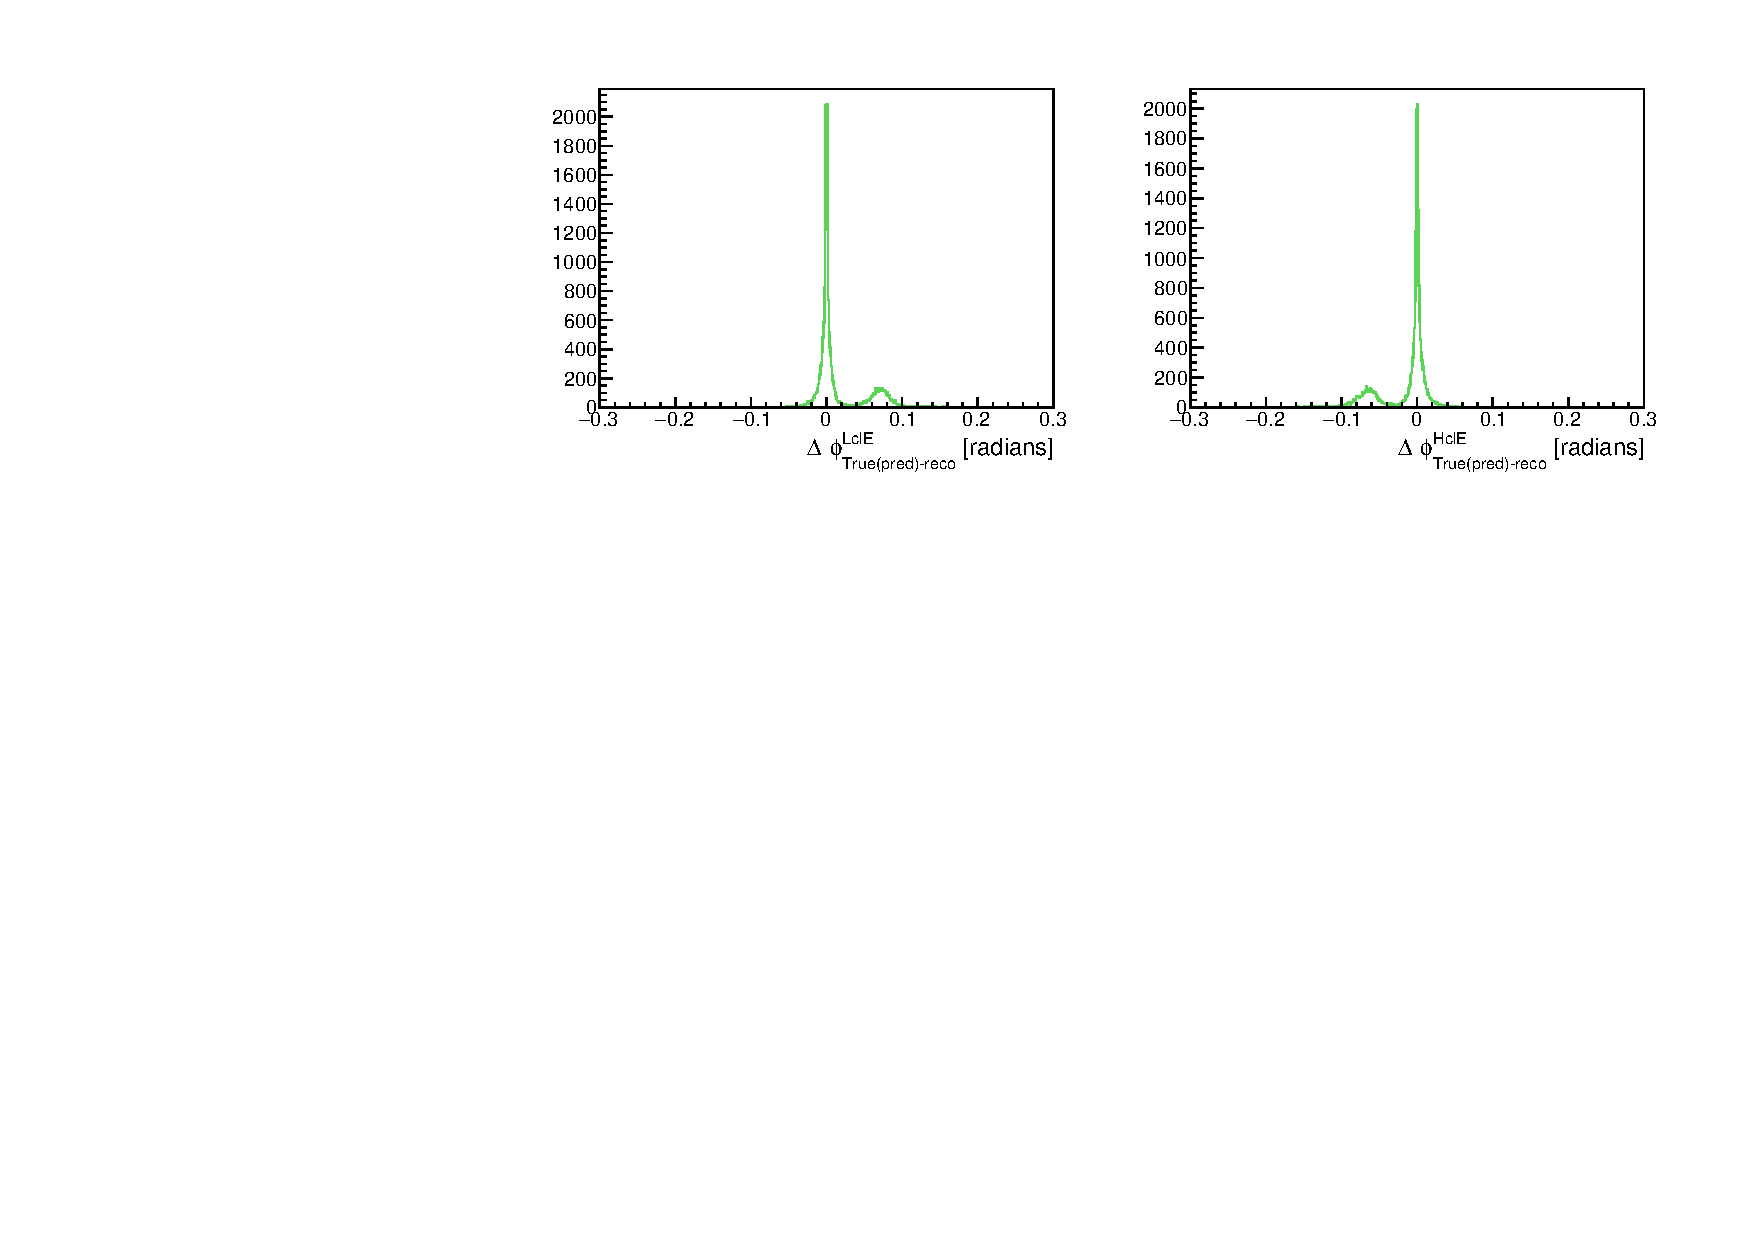
\includegraphics[width=\textwidth]{VBilder/b2b_MC}
\end{frame}

\begin{frame}
	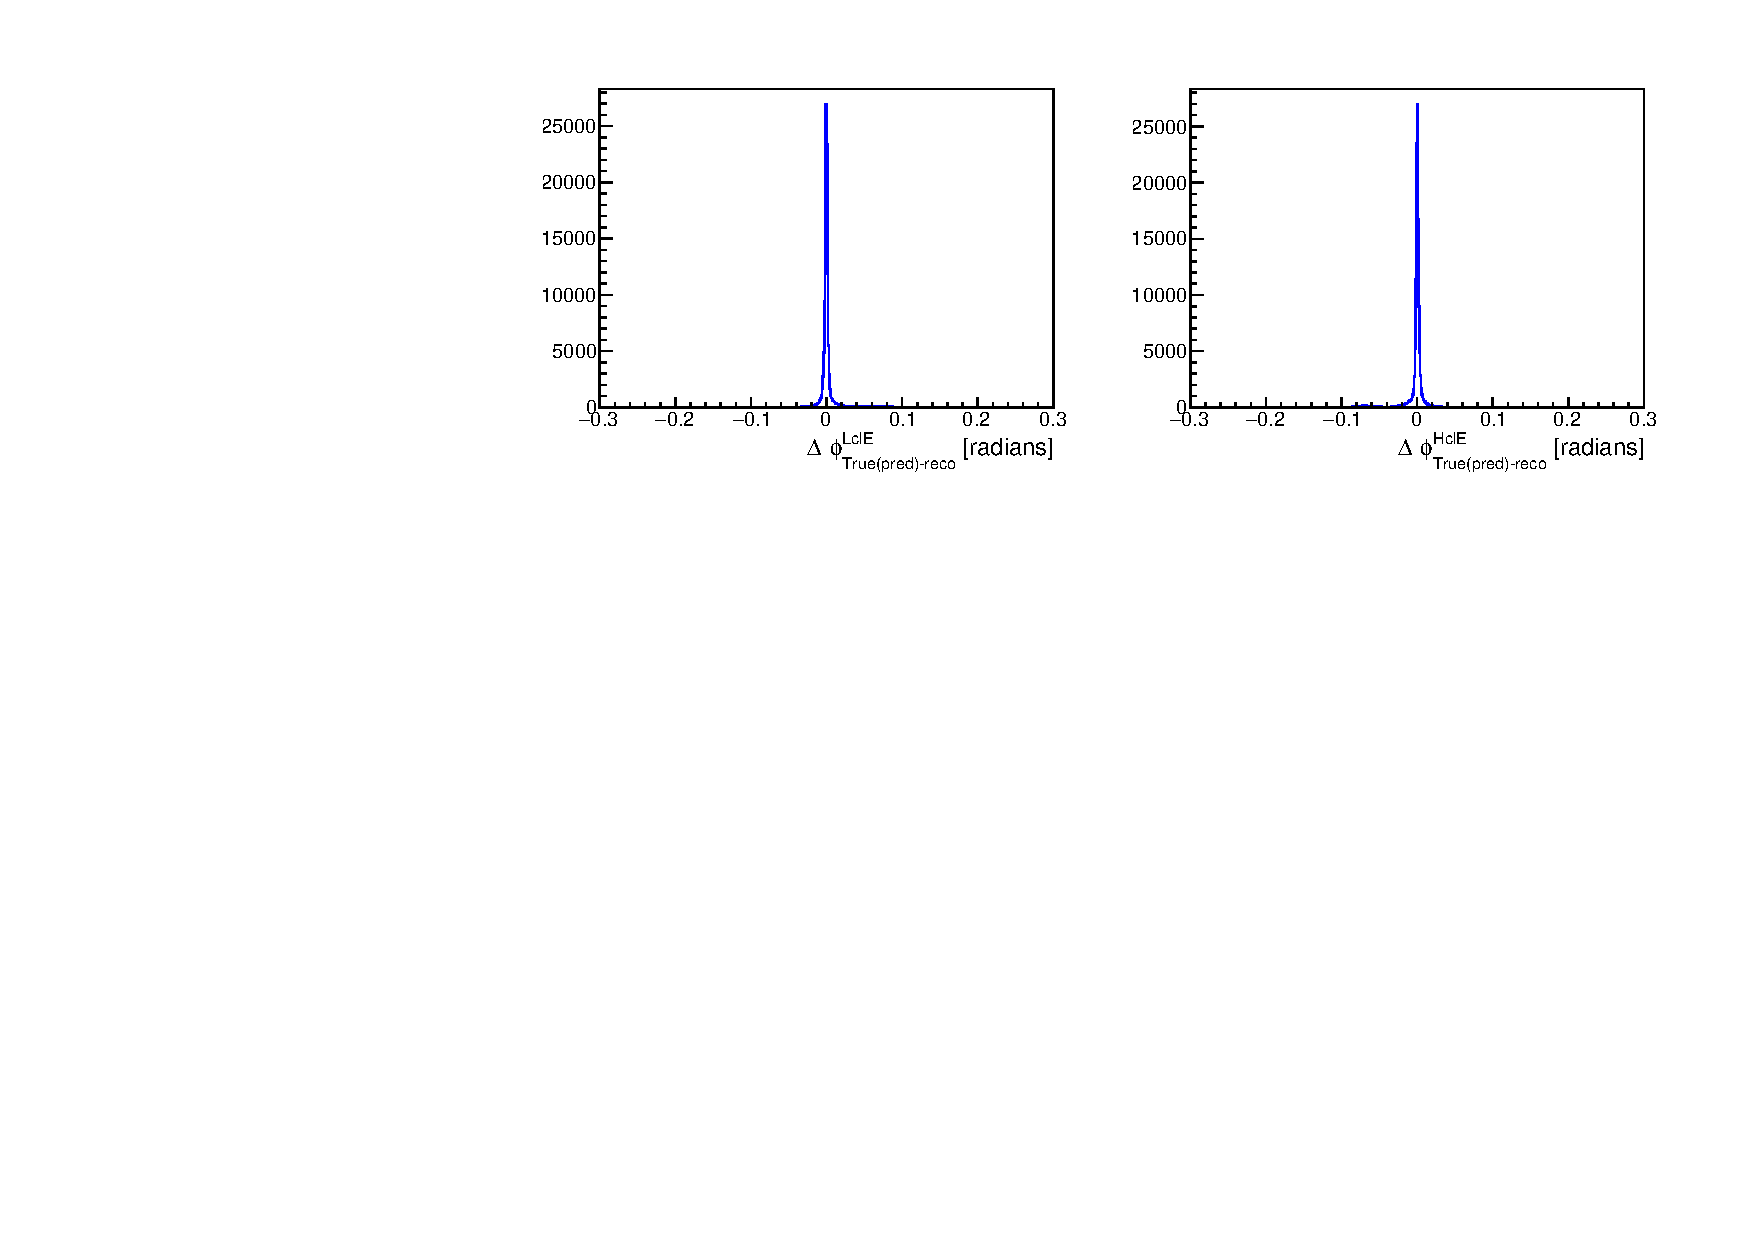
\includegraphics[width=\textwidth]{VBilder/b2b_DataP3}
	
	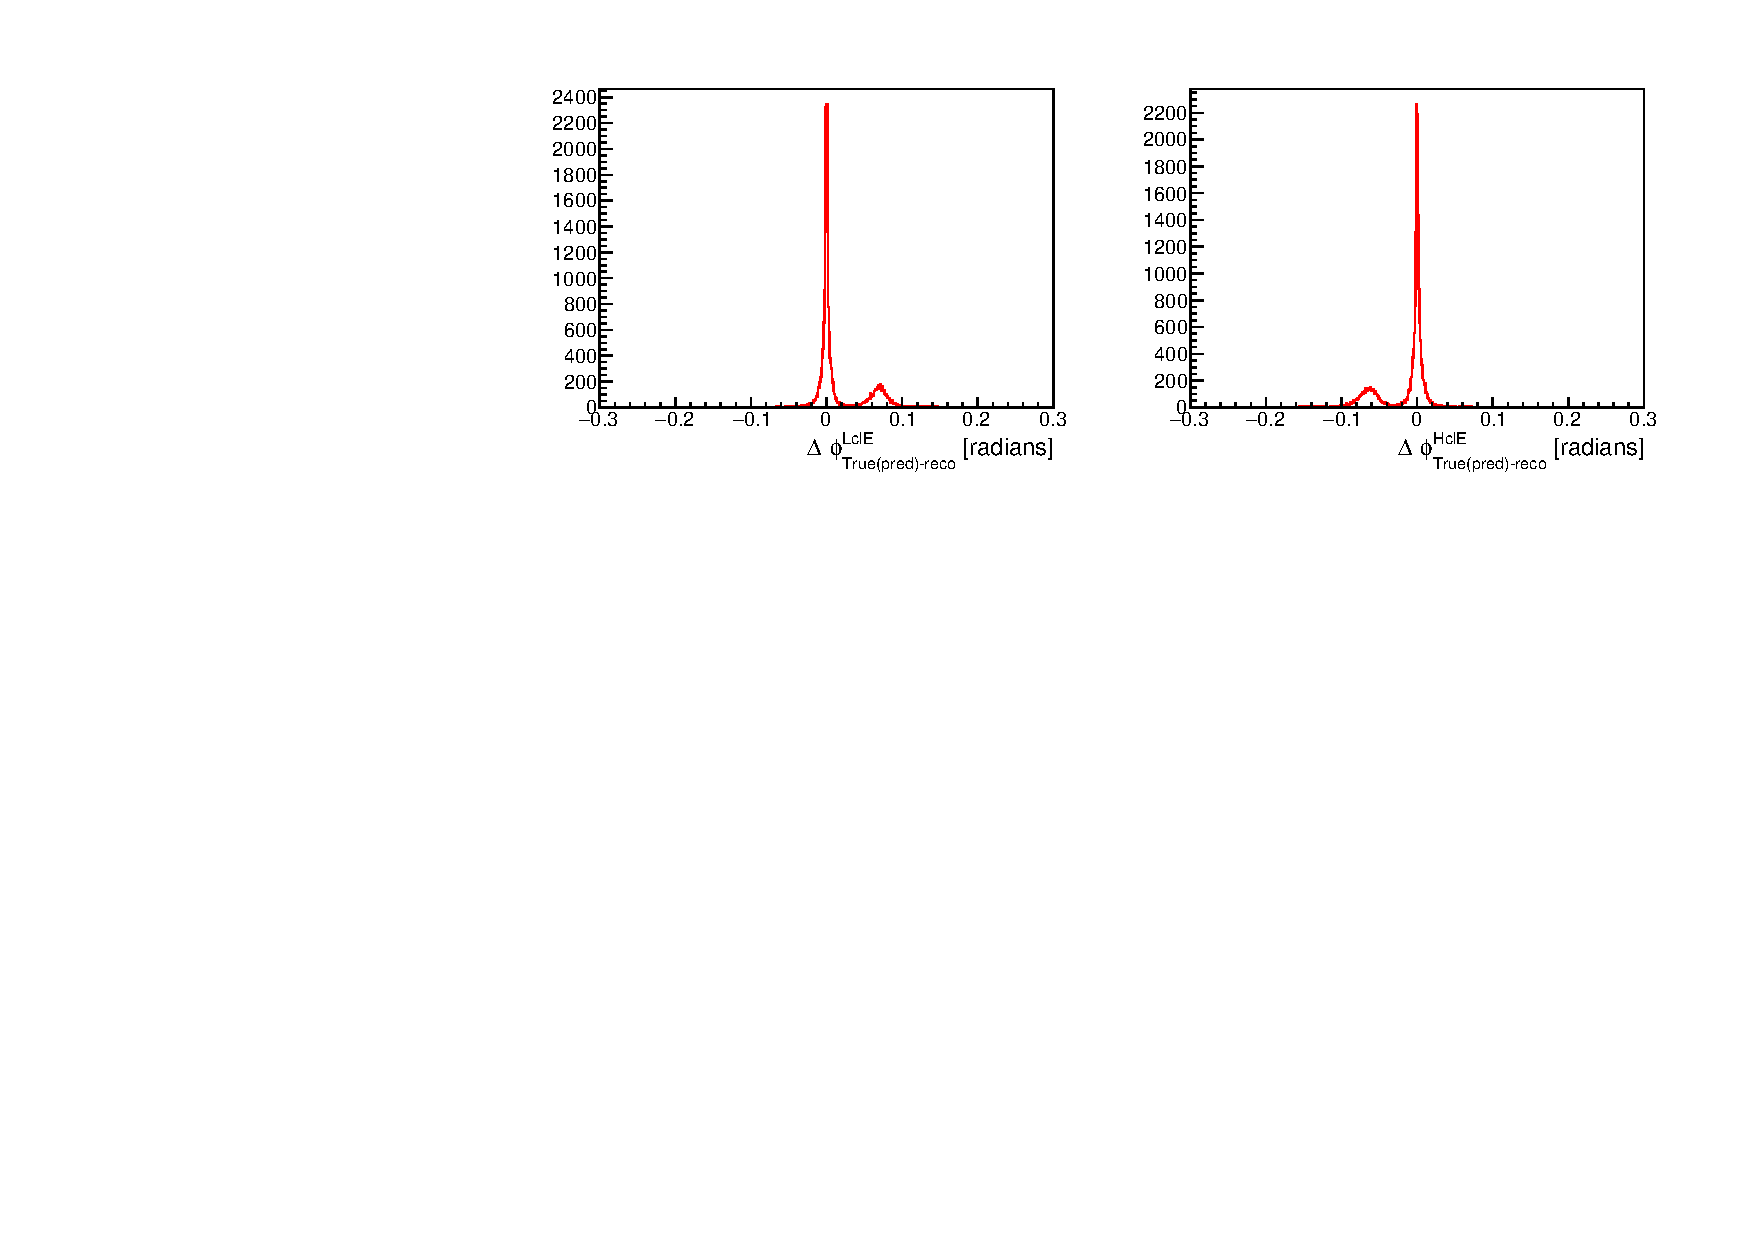
\includegraphics[width=\textwidth]{VBilder/b2b_MCP3}
\end{frame}






\section{Phase2 Tracking Efficiencies}


\begin{frame}{Phase2 Tracking Efficiencies As Function Of $\theta_{\textrm{pred,b2b}}-\phi_{\textrm{pred,b2b}}$}
	
	
	
	\begin{textblock*}{9cm}(1cm,-4cm)
		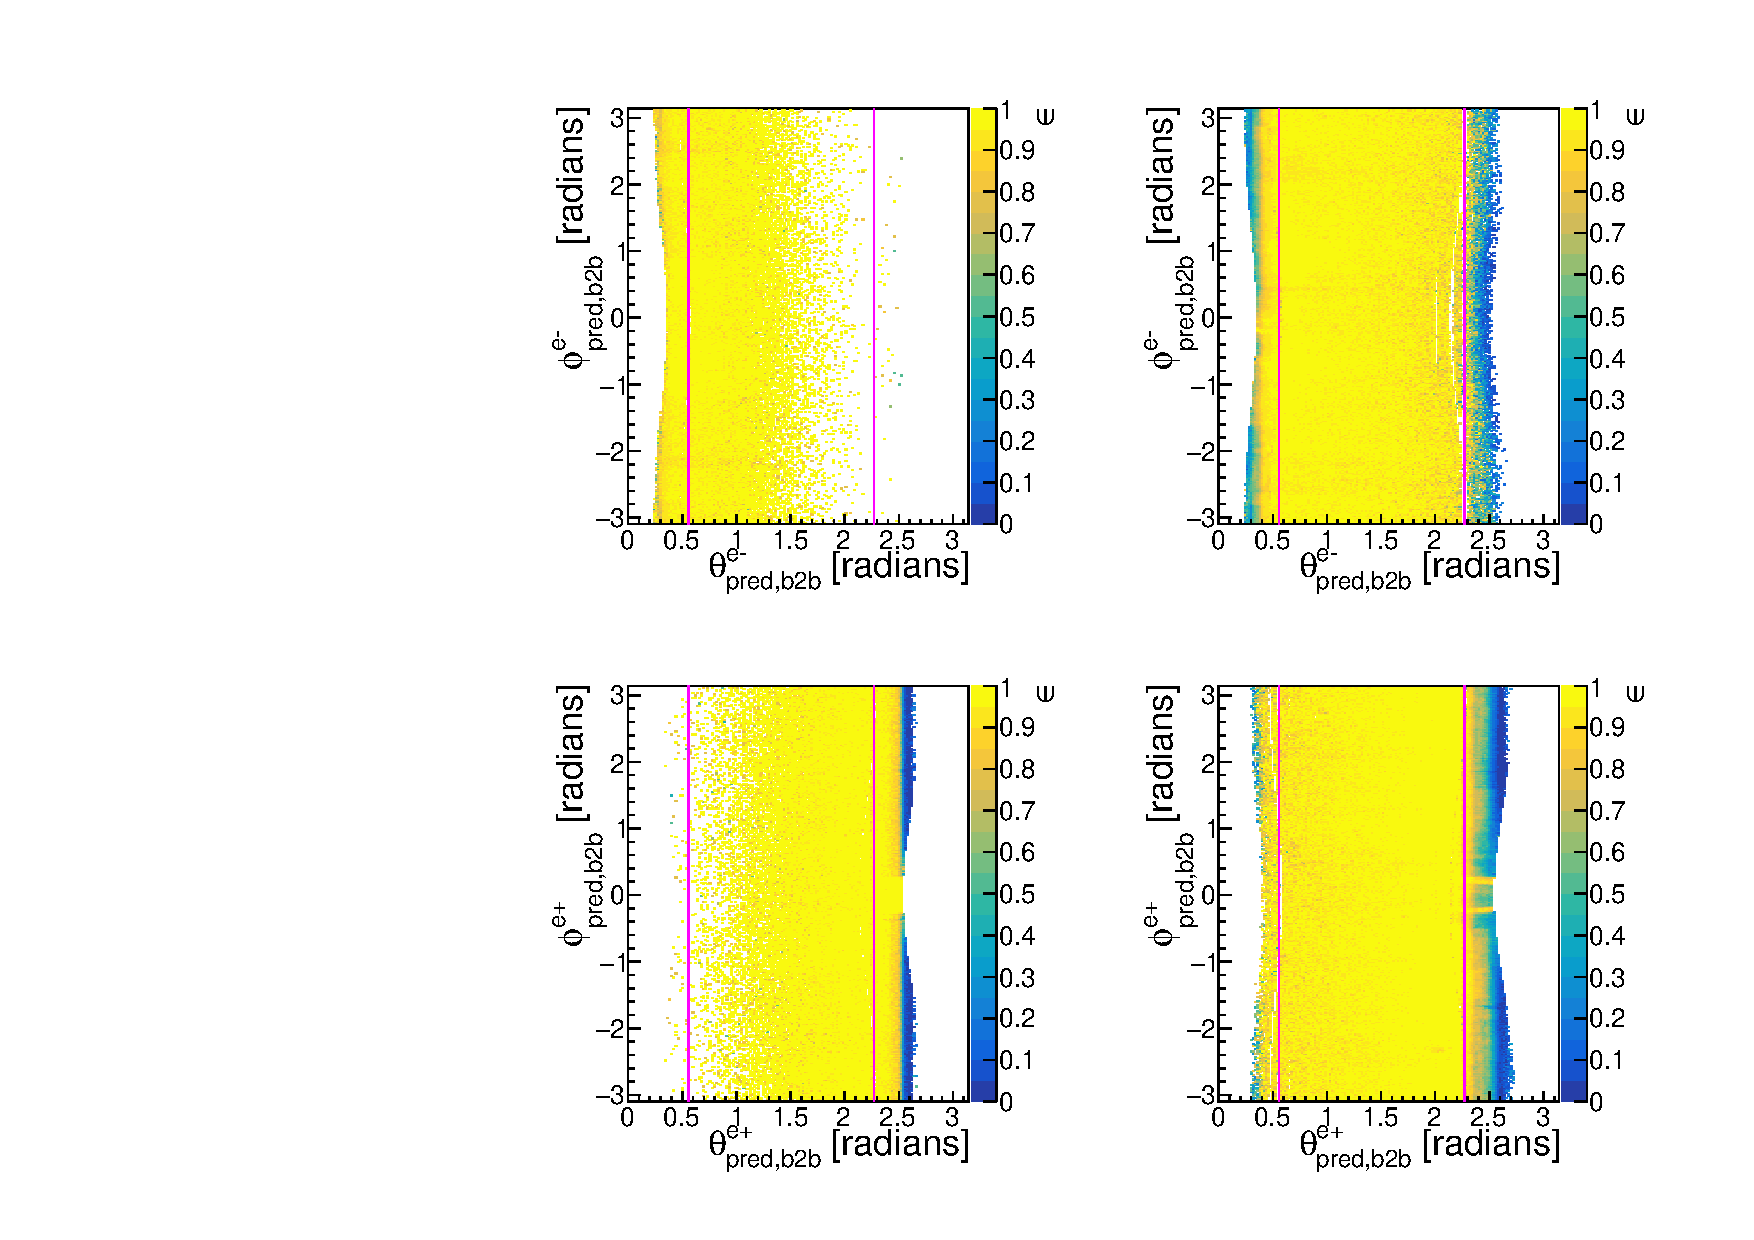
\includegraphics[width=\textwidth]{VPlots/P2/xCEffTP_MCData}
	\end{textblock*}
	
	\begin{textblock*}{2cm}(0cm,-2cm)
		$\textrm{e}^-$
	\end{textblock*}
	
	\begin{textblock*}{2cm}(0cm,2.3cm)
		$\textrm{e}^+$
	\end{textblock*}
	
	
	\begin{textblock*}{2cm}(2.8cm,-3.9cm)
		MC
	\end{textblock*}
	
	\begin{textblock*}{2cm}(7.2cm,-3.9cm)
		Data
	\end{textblock*}
	
	
	
	
	\begin{textblock*}{9cm}(1.8cm,-4cm)
		\begin{tikzpicture}
		\only<2>{
			\draw[line width=0.5mm,winered] \boundellipse{2cm,0cm}{0.2cm}{2cm};
		}
		\end{tikzpicture}
	\end{textblock*}
	
	\begin{textblock*}{9cm}(6.3cm,-4cm)
		\begin{tikzpicture}
		\only<2>{	
			\draw[line width=0.5mm,winered] \boundellipse{2cm,0cm}{0.2cm}{2cm};
		}
		\end{tikzpicture}
	\end{textblock*}
	
	
	\begin{textblock*}{8cm}(1.5cm,1cm)
		\only<2>{
			
			\begin{mybox}
				The tracking efficiency drops noticeably for phase2 data in contrast to phase2 MC
			\end{mybox}
			
		}
		
	\end{textblock*}
	
	
	\begin{textblock*}{9cm}(3.6cm,0.5cm)
		\begin{tikzpicture}
		\only<3>{
			\draw[line width=0.5mm,winered] \boundellipse{2cm,0cm}{0.2cm}{2cm};
		}
		\end{tikzpicture}
	\end{textblock*}
	
	\begin{textblock*}{9cm}(8.1cm,0.5cm)
		\begin{tikzpicture}
		\only<3>{	
			\draw[line width=0.5mm,winered] \boundellipse{2cm,0cm}{0.2cm}{2cm};
		}
		\end{tikzpicture}
	\end{textblock*}
	
	
	\begin{textblock*}{8cm}(1.5cm,-2cm)
		\only<3>{
			
			\begin{mybox}
				The tracking efficiency drops more sharp on phase2 MC.
				
				Also there is something like a \textit{horn} structure on phase2 data
			\end{mybox}
			
		}
		
	\end{textblock*}
	
	
	
	
\end{frame}



\begin{frame}{Phase2 Tracking Efficiencies As Function Of $\phi_{\textrm{pred,b2b}}$; Forward End-Cap}
	
	
	\begin{textblock*}{6.5cm}(-0.9cm,-3cm)
		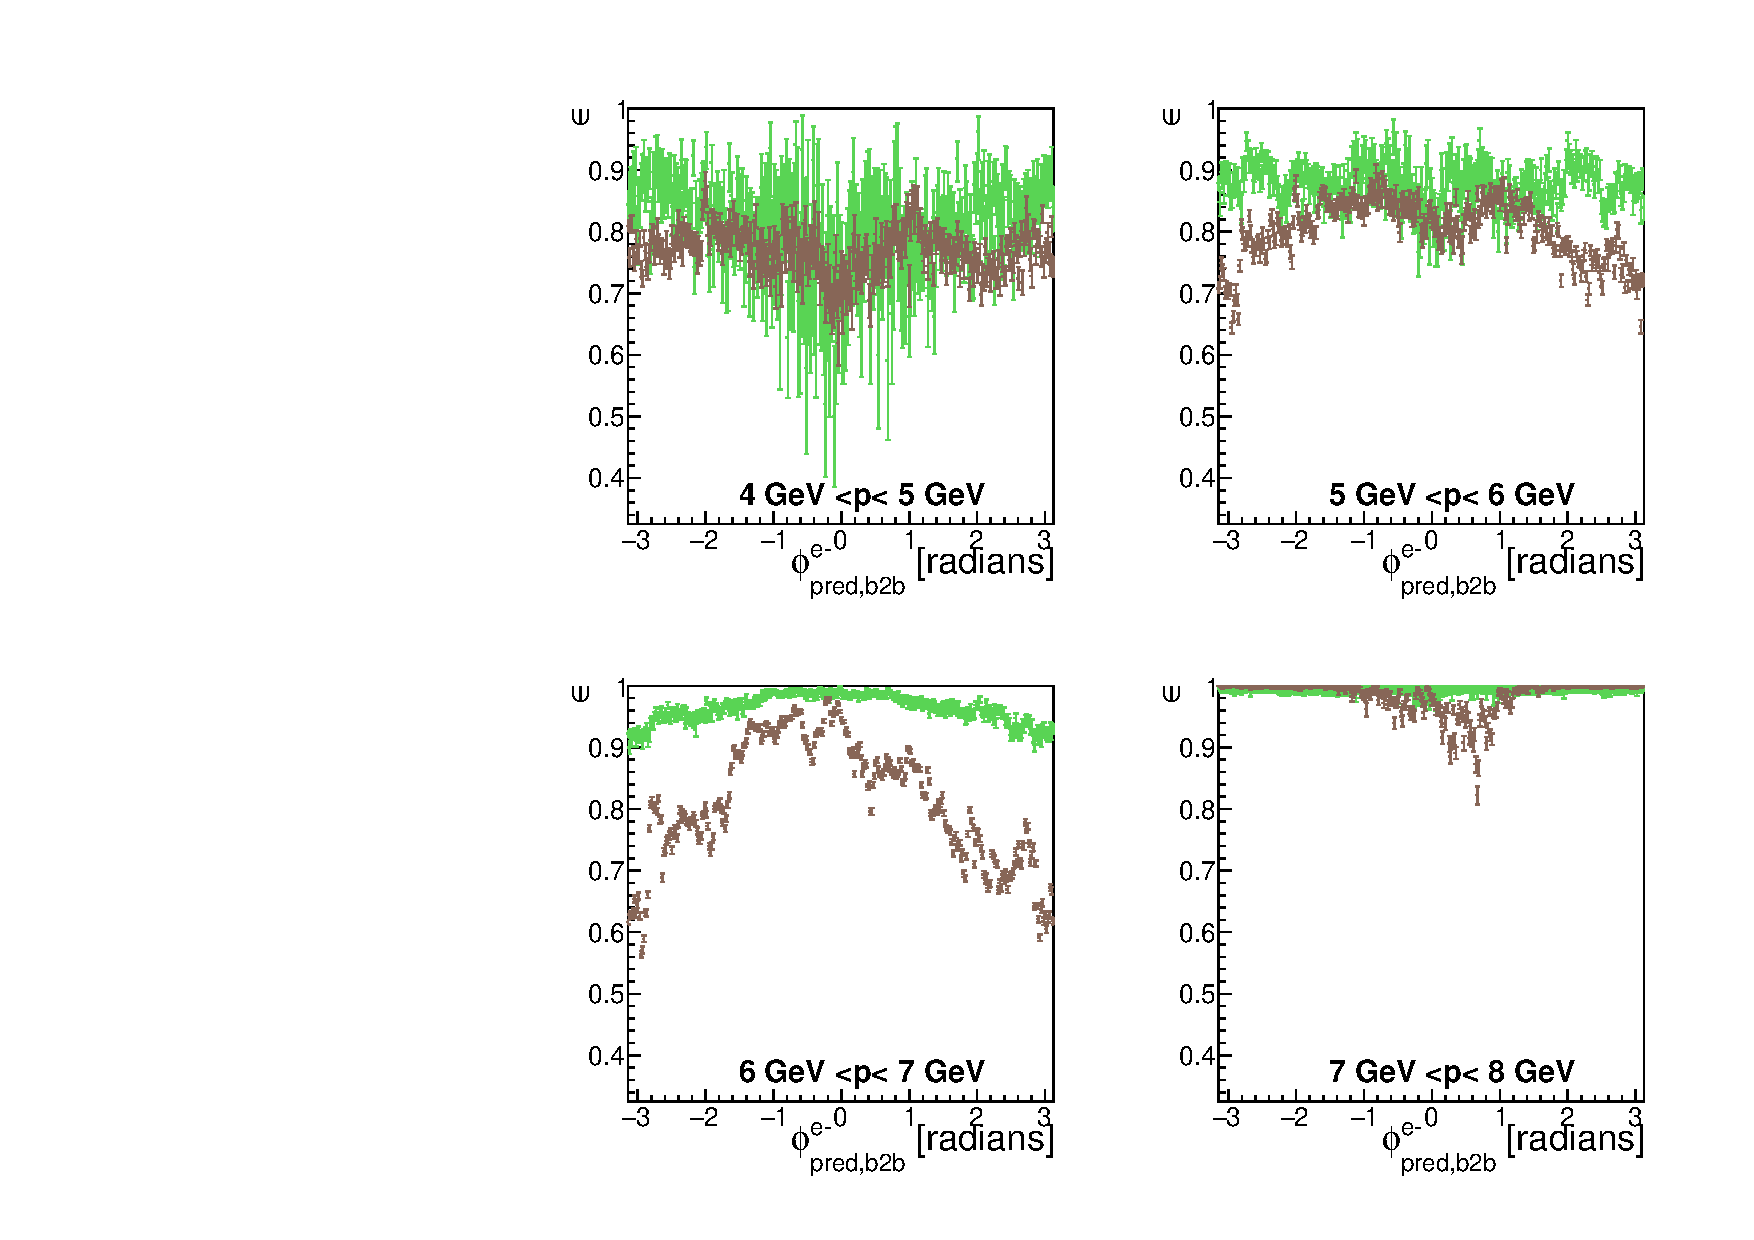
\includegraphics[width=\textwidth]{VPlots/P2/xPMPhiemFC}
	\end{textblock*}
	
	\begin{textblock*}{2cm}(2.3cm,-3.5cm)
		$\textrm{e}^-$
	\end{textblock*}
	
	\begin{textblock*}{2cm}(8.7cm,-3.5cm)
		$\textrm{e}^+$
	\end{textblock*}
	
	
	\begin{textblock*}{11cm}(5.5cm,-4.3cm)
		
		\begin{center}
			\line(0,1){256}
		\end{center}
		
	\end{textblock*}
	
	
	\begin{textblock*}{6.5cm}(6cm,-2.5cm)
		
		\setlength{\unitlength}{5cm}
		\begin{picture}(1,1)
		\put(0,0){\line(1,1){1}}
		
		\end{picture}
		
	\end{textblock*}
	
	
	
	\begin{textblock*}{4cm}(-0.5cm,-3.7cm)
		\textcolor{OliveGreen}{Phase2 MC10}
		
		\textcolor{brown}{Phase2 Data}
	\end{textblock*}
	
	
	\pause[2]
	
	\begin{textblock*}{6cm}(5.6cm,-3.5cm)
		\begin{mybox}
			Electron Tracking Efficiency:
			\begin{itemize}
				
				\item Phase2 MC has almost always a higher tracking efficiency compared to phase2 data
				\item For most momenta the biggest difference between phase2 MC and phase2 data occurs for $|\phi_{\textrm{pred,b2b}}| \gtrsim 2$
				
				\item<3-> There is no similarity in the structure for momenta between $6\,\textrm{GeV}$ and $7\,\textrm{GeV}$
				\item<4-> Highest tracking efficiency occurs for momenta between $7\,\textrm{GeV}$ and $8\,\textrm{GeV}$. But there is also an efficiency drop at $\phi_{\textrm{pred,b2b}} \gtrsim 0$
			\end{itemize}
		\end{mybox}
	\end{textblock*}
	\pause[3]
	\begin{textblock*}{5cm}(-1.2cm,-0.cm)
		\begin{tikzpicture}
		\only<3>{
			\draw[line width=0.5mm,winered] \boundellipse{2cm,0cm}{2.cm}{2.cm};
		}
		\end{tikzpicture}
	\end{textblock*}
	
	\begin{textblock*}{5cm}(3.3cm,.3cm)
		\begin{tikzpicture}
		\only<4>{
			\draw[line width=0.5mm,winered] \boundellipse{2cm,0cm}{.8cm}{.5cm};
		}
		\end{tikzpicture}
	\end{textblock*}
	
	
	\pause[5]
	
	
\end{frame}

\begin{frame}{Phase2 Tracking Efficiencies As Function Of $\phi_{\textrm{pred,b2b}}$; Barrel}
	
	
	\begin{textblock*}{6.5cm}(-0.9cm,-3cm)
		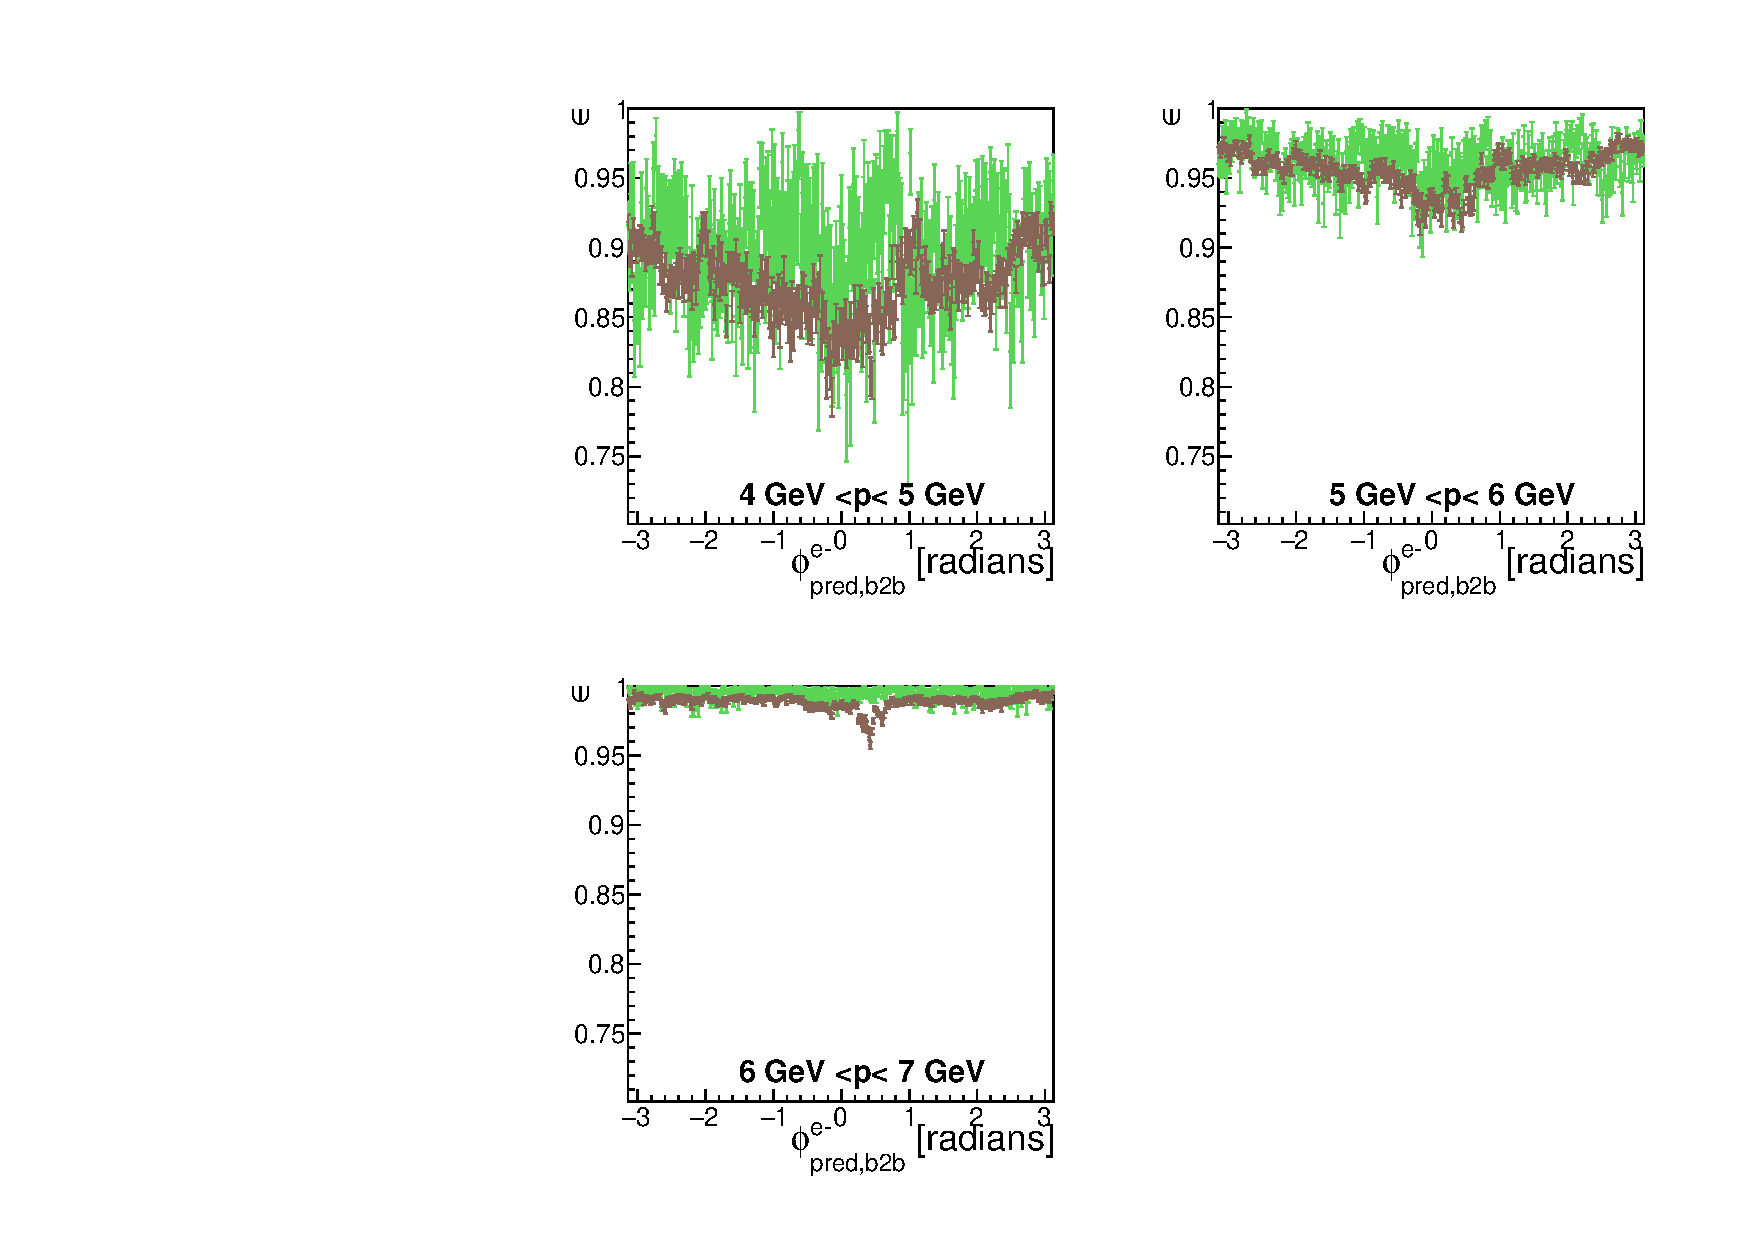
\includegraphics[width=\textwidth]{VPlots/P2/xPMPhiemBarrel}
	\end{textblock*}
	
	\begin{textblock*}{6.5cm}(5.5cm,-3cm)
		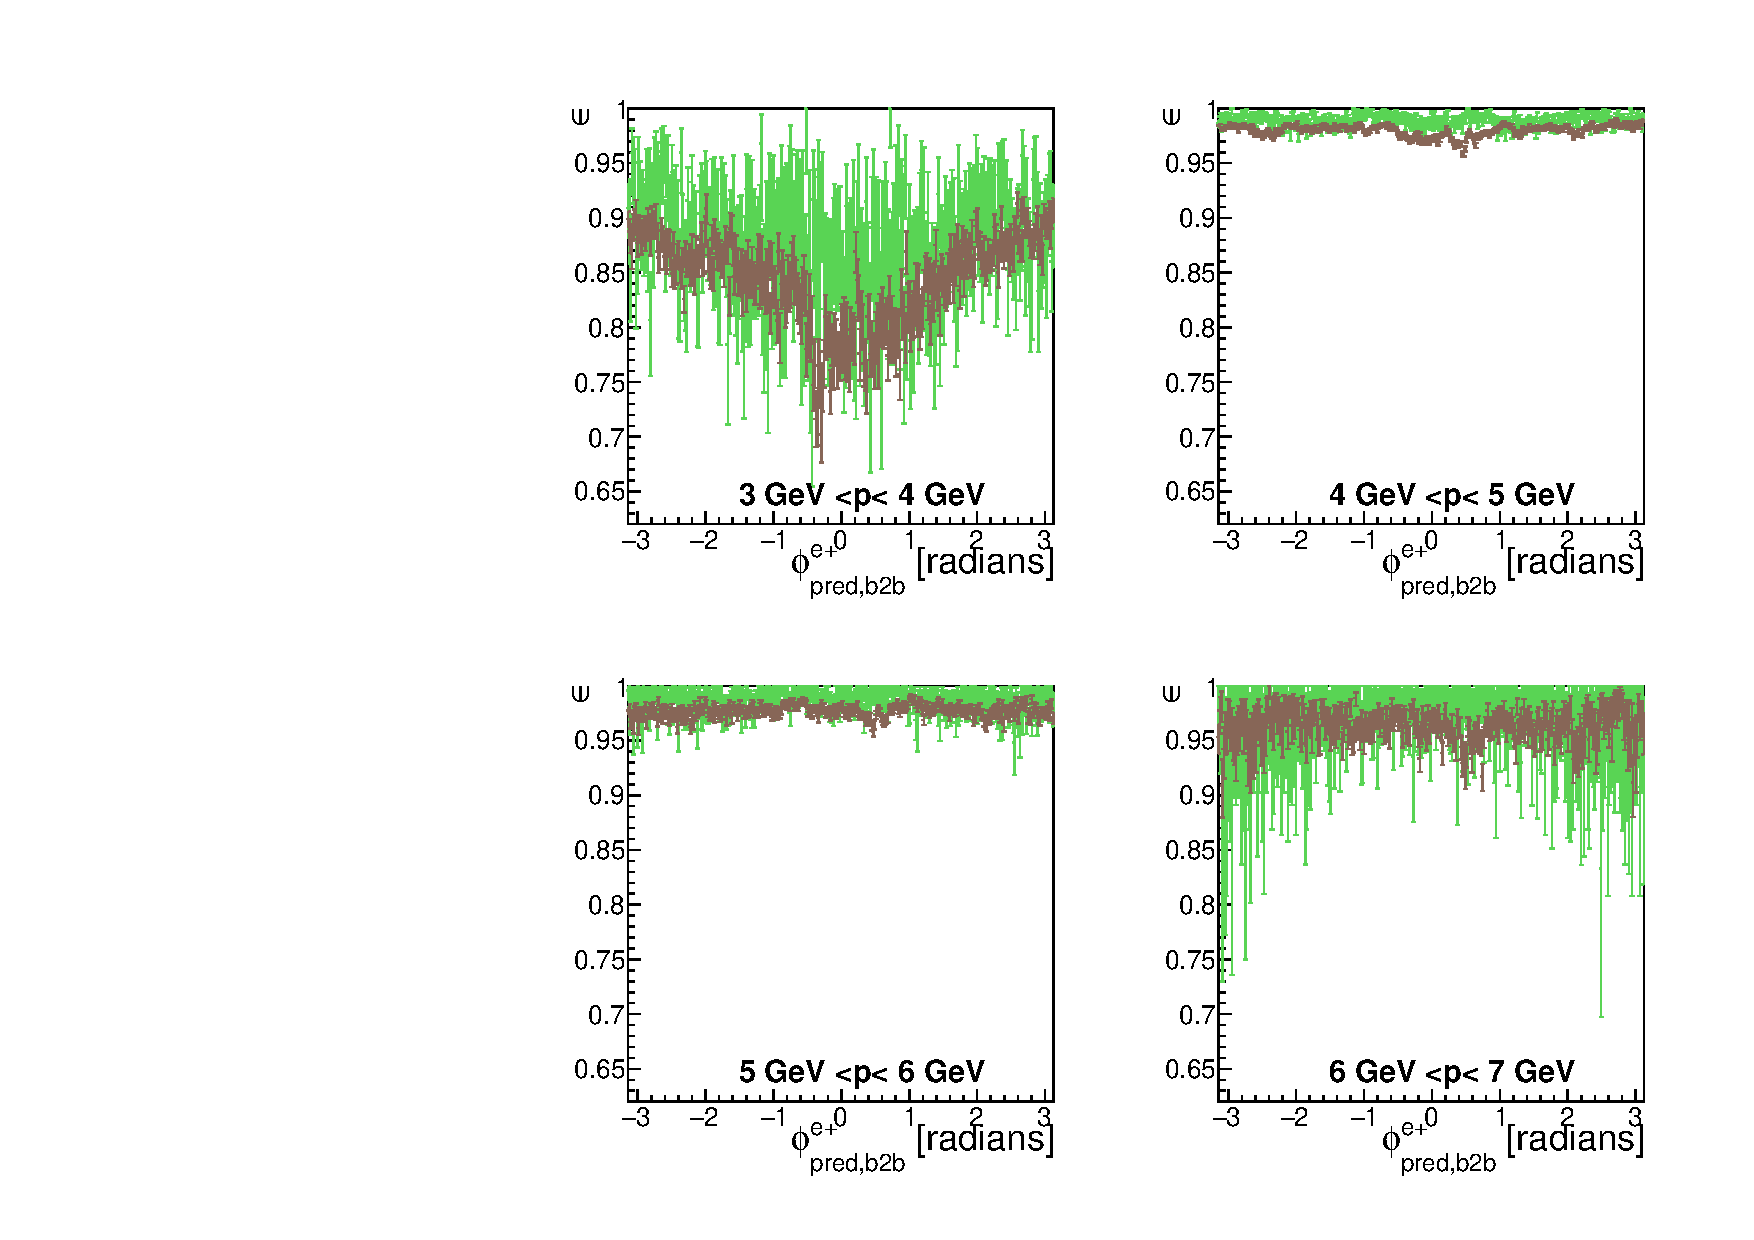
\includegraphics[width=\textwidth]{VPlots/P2/xPMPhiepBarrel}
	\end{textblock*}
	
	
	\begin{textblock*}{2cm}(2.3cm,-3.5cm)
		$\textrm{e}^-$
	\end{textblock*}
	
	\begin{textblock*}{2cm}(8.7cm,-3.5cm)
		$\textrm{e}^+$
	\end{textblock*}
	
	
	
	\begin{textblock*}{11cm}(5.5cm,-4.3cm)
		
		\begin{center}
			\line(0,1){256}
		\end{center}
		
	\end{textblock*}
	
	
	
	\begin{textblock*}{4cm}(-0.5cm,-3.7cm)
		\textcolor{OliveGreen}{Phase2 MC10}
		
		\textcolor{brown}{Phase2 Data}
	\end{textblock*}
	
	
	
	
	\begin{textblock*}{5cm}(0.65cm,0.4cm)
		\begin{tikzpicture}
		\only<2,3>
		{
			\draw[line width=0.5mm,winered] \boundellipse{2cm,0cm}{0.3cm}{.3cm};
		}
		\end{tikzpicture}
	\end{textblock*}
	
	\begin{textblock*}{5cm}(0.65cm,-3cm)
		\begin{tikzpicture}
		\only<2>
		{
			\draw[line width=0.5mm,winered] \boundellipse{2cm,0cm}{0.3cm}{1.5cm};
		}
		\end{tikzpicture}
	\end{textblock*}
	
	\begin{textblock*}{5cm}(3.9cm,-3cm)
		\begin{tikzpicture}
		\only<2>{
			\draw[line width=0.5mm,winered] \boundellipse{2cm,0cm}{0.3cm}{1.cm};
		}
		\end{tikzpicture}
	\end{textblock*}
	
	
	
	
	
	\begin{textblock*}{6cm}(5.6cm,-3.5cm)
		\only<2,3,4>{
			\begin{mybox}
				Electron Tracking Efficiency:
				\begin{itemize}
					
					\item<2-> The highest tracking efficiency occurs for momenta between $6\,\textrm{GeV}$ and $7\,\textrm{GeV}$
					\item<2-> There is a slope at $\phi_{\textrm{pred,b2b}} \gtrsim 0$ for phase2 MC and phase2 data
					\item<3-> This kind of drop we also saw in the forward end-cap for momenta between  $7\,\textrm{GeV}$ and $8\,\textrm{GeV}$
				\end{itemize}
			\end{mybox}
		}
	\end{textblock*}
	
	
	\begin{textblock*}{6cm}(-0.7cm,-3.5cm)
		\only<5->{
			\begin{mybox}
				Positron Tracking Efficiency:
				\begin{itemize}
					
					\item The highest tracking efficiency occurs for momenta between $4\,\textrm{GeV}$ and $5\,\textrm{GeV}$
					\item The lowest tracking efficiency occurs for momenta between $3\,\textrm{GeV}$ and $4\,\textrm{GeV}$ with a minima at $\phi_{\textrm{pred,b2b}} \approx 0$
				\end{itemize}
			\end{mybox}
		}
	\end{textblock*}
	
	
	
	
	
	
\end{frame}



\begin{frame}{Phase2 Tracking Efficiencies As Function Of $\phi_{\textrm{pred,b2b}}$; Backward End-Cap}
	
	
	\begin{textblock*}{6.5cm}(5.5cm,-3cm)
		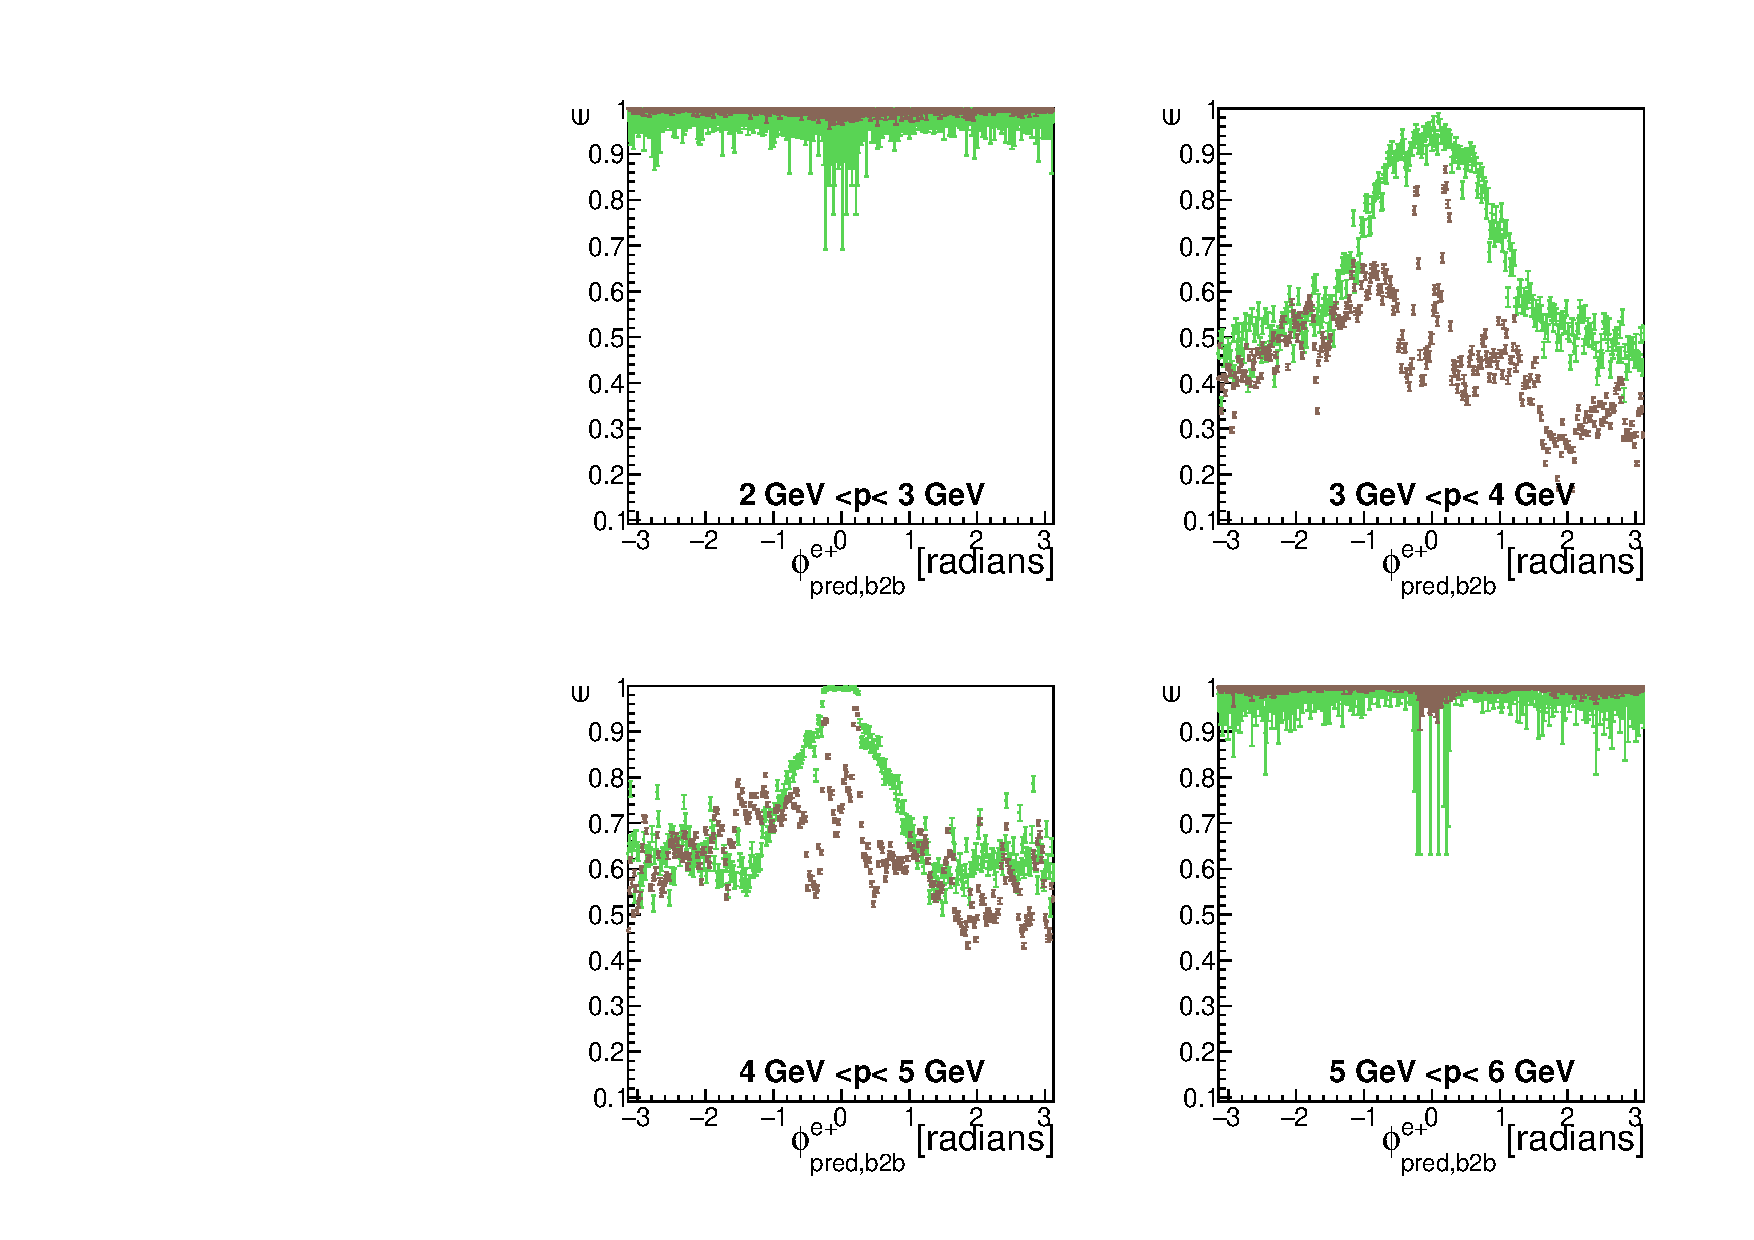
\includegraphics[width=\textwidth]{VPlots/P2/xPMPhiepEC}
	\end{textblock*}
	
	\begin{textblock*}{2cm}(2.3cm,-3.5cm)
		$\textrm{e}^-$
	\end{textblock*}
	
	\begin{textblock*}{2cm}(8.7cm,-3.5cm)
		$\textrm{e}^+$
	\end{textblock*}
	
	
	\begin{textblock*}{11cm}(5.5cm,-4.3cm)
		
		\begin{center}
			\line(0,1){256}
		\end{center}
		
	\end{textblock*}
	
	
	\begin{textblock*}{6.5cm}(-0.2cm,-2.5cm)
		
		\setlength{\unitlength}{5cm}
		\begin{picture}(1,1)
		\put(0,0){\line(1,1){1}}
		
		\end{picture}
		
	\end{textblock*}
	\only<1>{	
		\begin{textblock*}{4cm}(-0.5cm,-3.7cm)
			\textcolor{OliveGreen}{Phase2 MC10}
			
			\textcolor{brown}{Phase2 Data}
		\end{textblock*}
	}
	
	\only<2->{
		\begin{textblock*}{4cm}(6cm,-3.7cm)
			\textcolor{OliveGreen}{Phase2 MC10}
			
			\textcolor{brown}{Phase2 Data}
		\end{textblock*}
		
	}
	
	
	
	
	\pause 
	
	
	\begin{textblock*}{6cm}(-0.7cm,-3.5cm)
		\only<2->{
			\begin{mybox}
				Positron Tracking Efficiency:
				\begin{itemize}
					
					\item The highest tracking efficiency occurs for momenta between $2\,\textrm{GeV}$ and $3\,\textrm{GeV}$ and $5\,\textrm{GeV}$ and $6\,\textrm{GeV}$
					\item<3-> Weird \textit{horn} structure we saw earlier
					\item<3-> Phase2 MC tracking efficiency peaks at $\phi_{\textrm{pred,b2b}} \approx 0$
					\item<4> For momenta between $4\,\textrm{GeV}$ and $5\,\textrm{GeV}$ phase2 data appears to have a higher tracking efficiency compared to phase2 MC at $\phi_{\textrm{pred,b2b}} \approx -1$
					
				\end{itemize}
			\end{mybox}
		}
	\end{textblock*}
	
	\begin{textblock*}{5cm}(9.9cm,-3cm)
		\begin{tikzpicture}
		\only<3>{
			\draw[line width=0.5mm,winered] \boundellipse{2cm,0cm}{0.6cm}{1.5cm};
		}
		\end{tikzpicture}
	\end{textblock*}
	
	\begin{textblock*}{5cm}(6.6cm,.2cm)
		\begin{tikzpicture}
		\only<3>{
			\draw[line width=0.5mm,winered] \boundellipse{2cm,0cm}{0.6cm}{1.5cm};
		}
		\end{tikzpicture}
	\end{textblock*}
	
	\begin{textblock*}{5cm}(6.3cm,.9cm)
		\begin{tikzpicture}
		\only<4>{
			\draw[line width=0.5mm,winered] \boundellipse{2cm,0cm}{0.4cm}{.4cm};
		}
		\end{tikzpicture}
	\end{textblock*}
	
	
	
	
\end{frame}


\begin{frame}{Phase2 Tracking Efficiencies As Function Of $\theta_{\textrm{pred,b2b}}$}
	
	
	\begin{textblock*}{6.5cm}(-0.9cm,-3cm)
		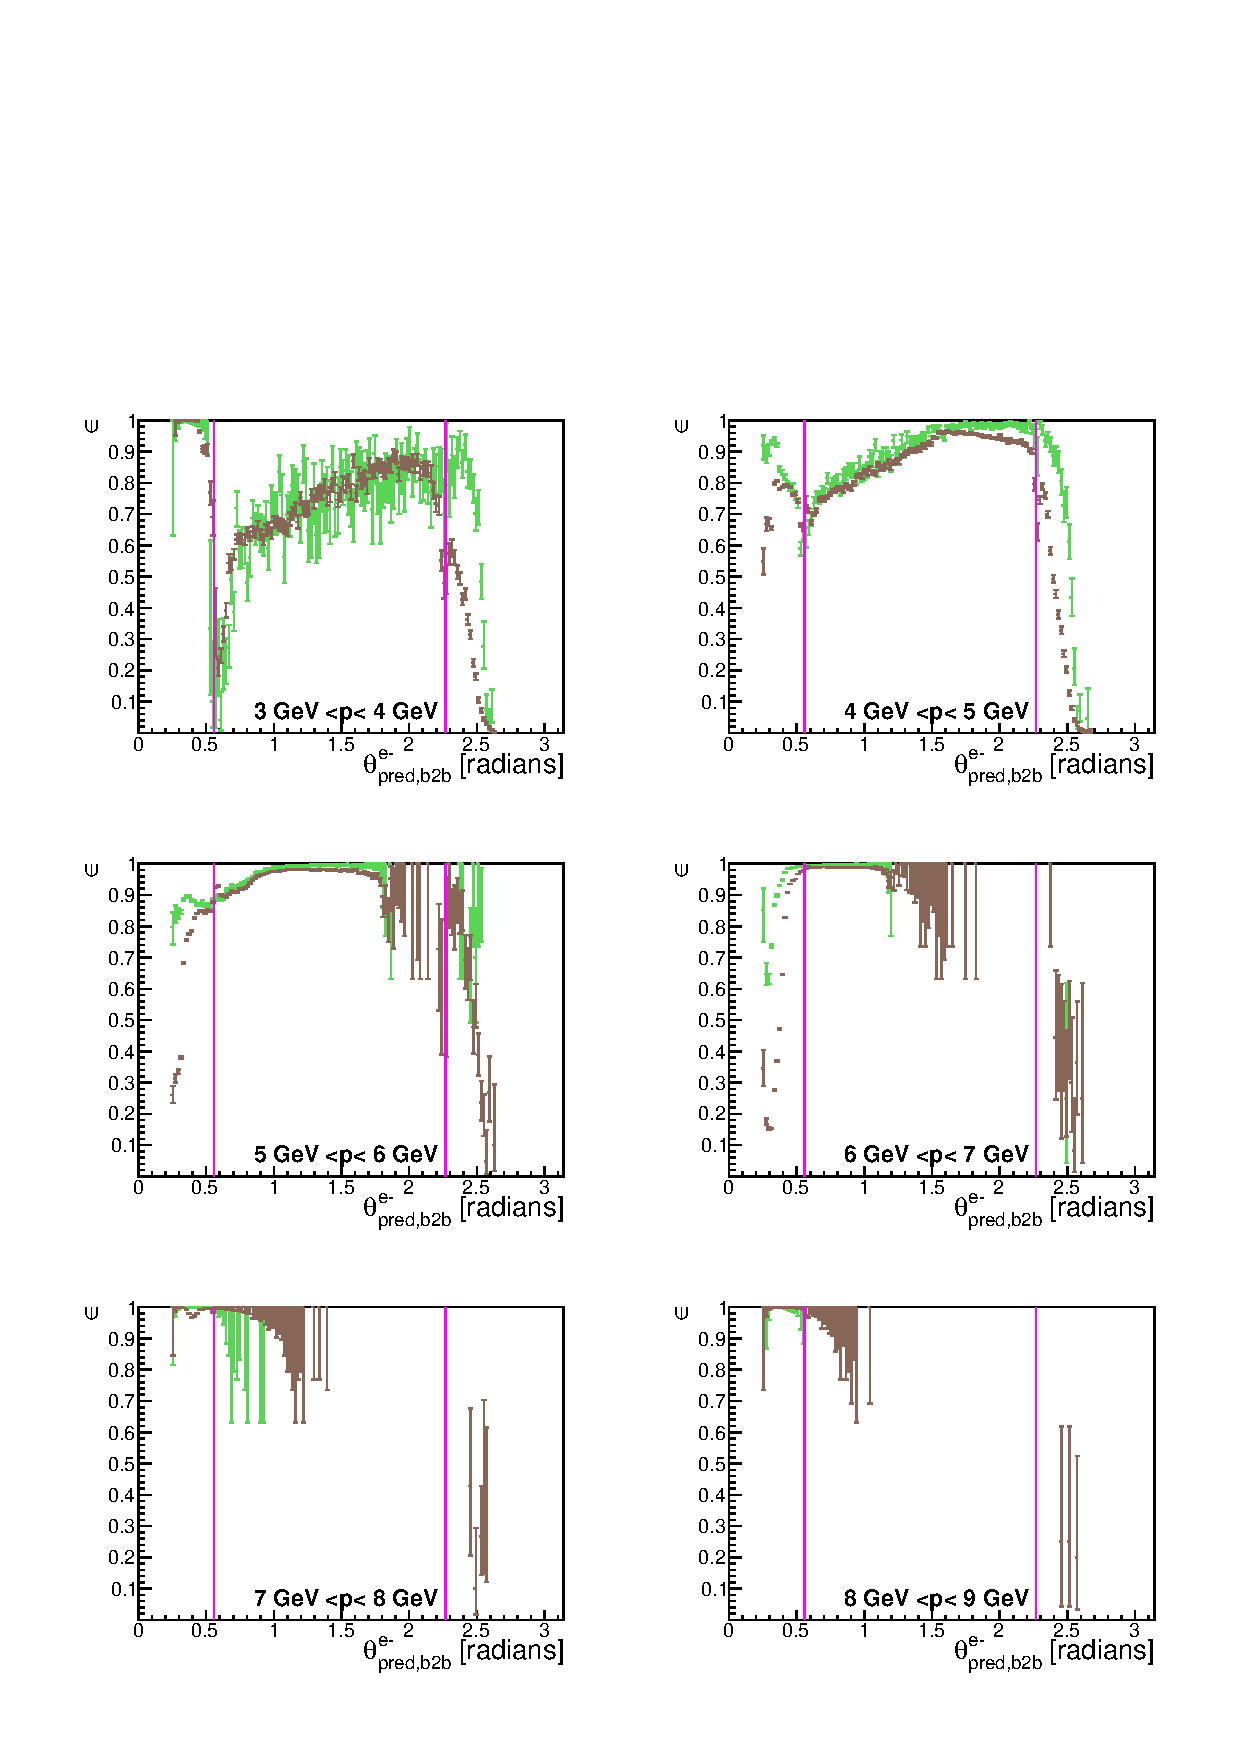
\includegraphics[width=\textwidth]{VPlots/P2/xPMThetaem}
	\end{textblock*}
	
	\begin{textblock*}{6.5cm}(5.5cm,-3cm)
		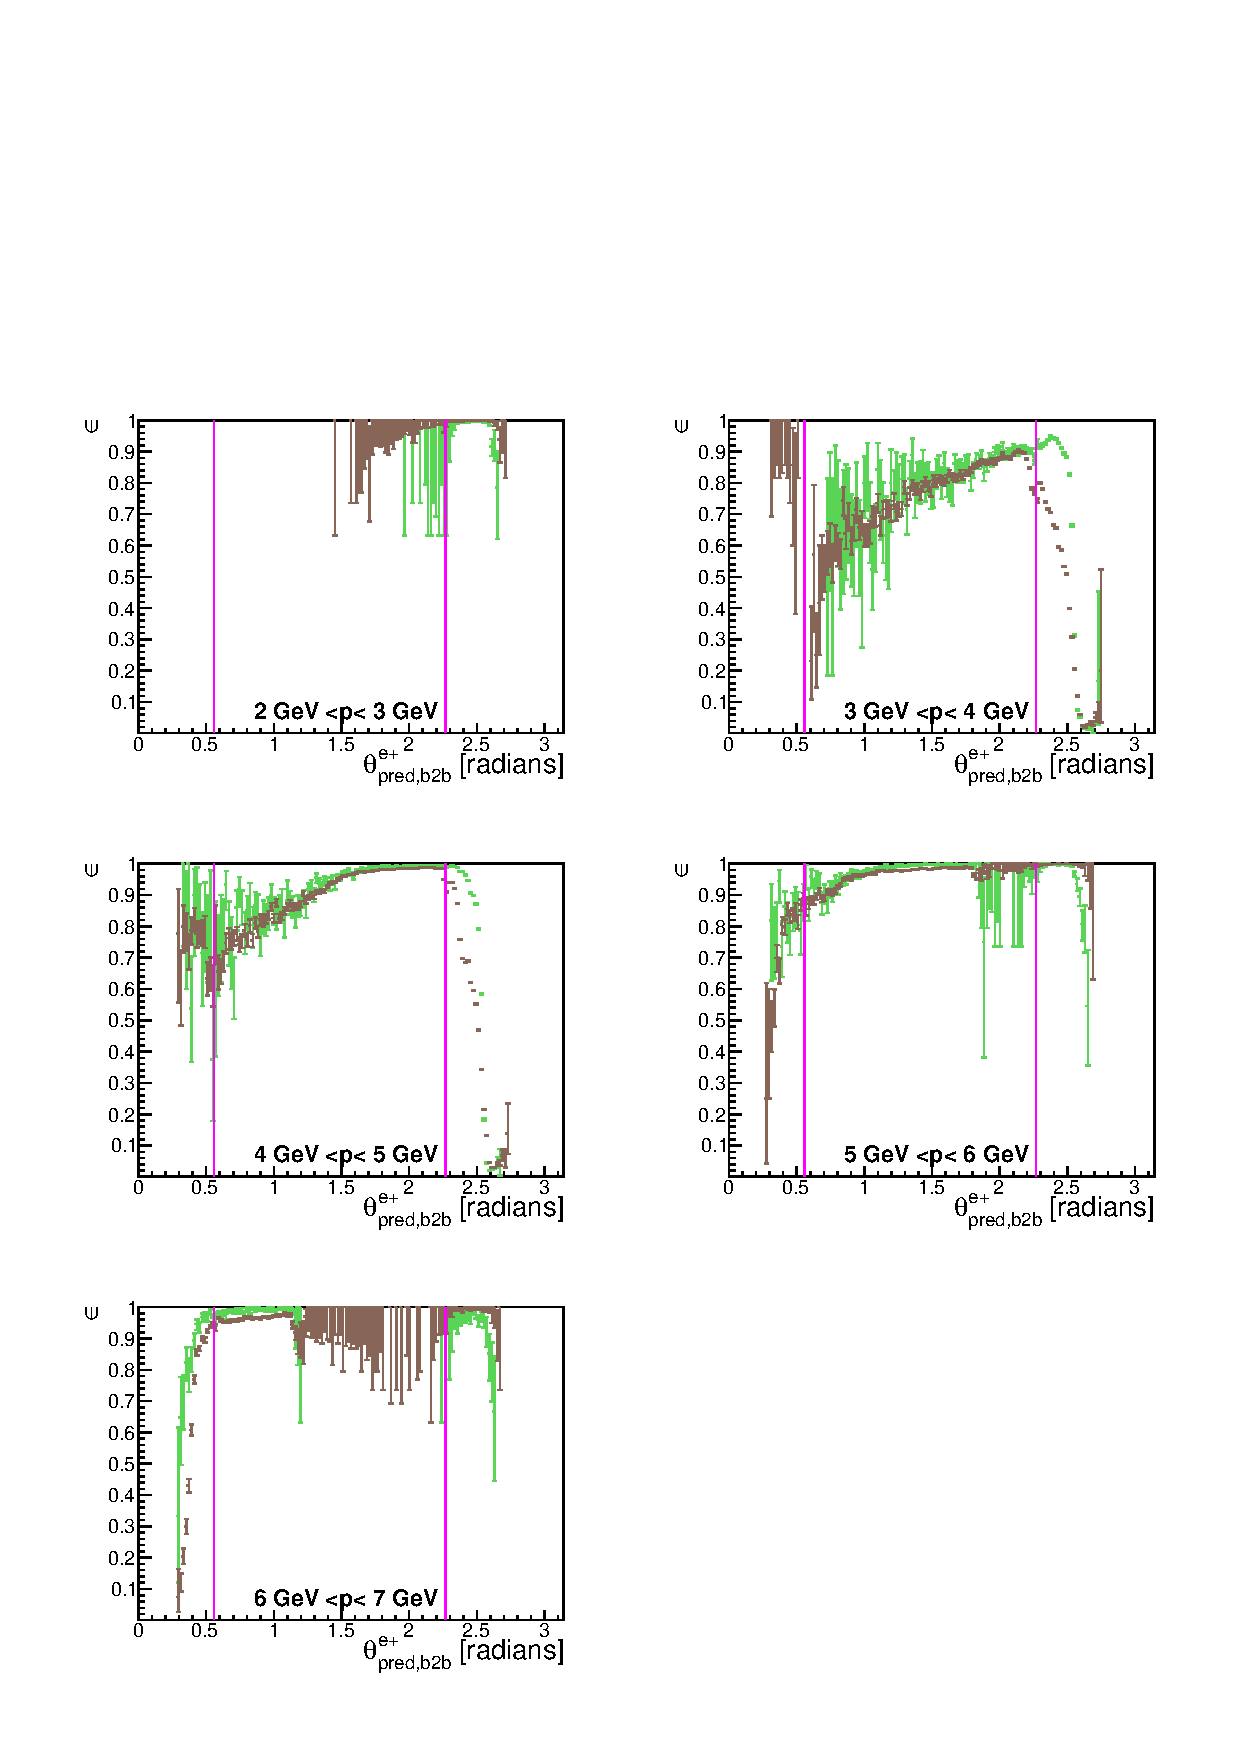
\includegraphics[width=\textwidth]{VPlots/P2/xPMThetaep}
	\end{textblock*}
	
	
	\begin{textblock*}{2cm}(2.3cm,-3.5cm)
		$\textrm{e}^-$
	\end{textblock*}
	
	\begin{textblock*}{2cm}(8.7cm,-3.5cm)
		$\textrm{e}^+$
	\end{textblock*}
	
	
	
	\begin{textblock*}{11cm}(5.5cm,-4.3cm)
		
		\begin{center}
			\line(0,1){256}
		\end{center}
		
	\end{textblock*}
	
	
	
	\only<1,2,3,4,5,6,7>{
		\begin{textblock*}{4cm}(-0.5cm,-3.7cm)
			\textcolor{OliveGreen}{Phase2 MC10}
			
			\textcolor{brown}{Phase2 Data}
		\end{textblock*}
	}
	
	
	\only<8->{
		
		
		\begin{textblock*}{4cm}(6cm,-3.7cm)
			\textcolor{OliveGreen}{Phase2 MC10}
			
			\textcolor{brown}{Phase2 Data}
		\end{textblock*}
		
		
		
	}
	
	
	
	
	
	
	
	
	\pause
	
	
	\only<2,3,4,5,6,7>{
		\begin{textblock*}{6cm}(5.6cm,-3.5cm)
			\begin{mybox}
				Electron Tracking Efficiency:
				\begin{itemize}
					\item<2,3,4,5,6> For momenta between $3\,\textrm{GeV}$ and $5\,\textrm{GeV}$ the tracking efficiency in the backward end-cap is worse for phase2 data compared to phase2 MC
					\item<3,4,5,6> For momenta between $4\,\textrm{GeV}$ and $6\,\textrm{GeV}$ the tracking efficiency in the forward end-cap is worse for phase2 data compared to phase2 MC
					\item<4,5,6> Drops in efficiency at transition between barrel and end-caps
					\item<5,6> A efficiency drop appears to propagate for momenta between $5\,\textrm{GeV}$ and $7\,\textrm{GeV}$ for phase2 data
					\item<6> There is a slope in the barrel
				\end{itemize}
			\end{mybox}
		\end{textblock*}
	}
	\begin{textblock*}{5cm}(1.2cm,-2.8cm)
		\begin{tikzpicture}
		\only<2>{
			\draw[line width=0.5mm,winered] \boundellipse{2cm,0cm}{0.3cm}{1.cm};
		}
		\end{tikzpicture}
	\end{textblock*}
	
	
	\begin{textblock*}{5cm}(4.4cm,-2.8cm)
		\begin{tikzpicture}
		\only<2>{
			\draw[line width=0.5mm,winered] \boundellipse{2cm,0cm}{0.3cm}{1.cm};
		}
		\end{tikzpicture}
	\end{textblock*}
	
	
	\begin{textblock*}{5cm}(2.8cm,-2.8cm)
		\begin{tikzpicture}
		\only<3>{
			\draw[line width=0.5mm,winered] \boundellipse{2cm,0cm}{0.3cm}{1.cm};
		}
		\end{tikzpicture}
	\end{textblock*}	
	
	
	\begin{textblock*}{5cm}(2.8cm,-0.4cm)
		\begin{tikzpicture}
		\only<3>{
			\draw[line width=0.5mm,winered] \boundellipse{2cm,0cm}{0.3cm}{1.cm};
		}
		\end{tikzpicture}
	\end{textblock*}	
	
	\begin{textblock*}{5cm}(-0.4cm,-0.4cm)
		\begin{tikzpicture}
		\only<3>{
			\draw[line width=0.5mm,winered] \boundellipse{2cm,0cm}{0.3cm}{1.cm};
		}
		\end{tikzpicture}
	\end{textblock*}
	
	
	\begin{textblock*}{5cm}(-0.2cm,-2.8cm)
		\begin{tikzpicture}
		\only<4>{
			\draw[line width=0.5mm,winered] \boundellipse{2cm,0cm}{0.3cm}{1.cm};
		}
		\end{tikzpicture}
	\end{textblock*}
	
	\begin{textblock*}{5cm}(1.cm,-2.8cm)
		\begin{tikzpicture}
		\only<4>{
			\draw[line width=0.5mm,winered] \boundellipse{2cm,0cm}{0.3cm}{1.cm};
		}
		\end{tikzpicture}
	\end{textblock*}
	
	\begin{textblock*}{5cm}(3cm,-2.8cm)
		\begin{tikzpicture}
		\only<4>{
			\draw[line width=0.5mm,winered] \boundellipse{2cm,0cm}{0.3cm}{1.cm};
		}
		\end{tikzpicture}
	\end{textblock*}
	
	
	\begin{textblock*}{5cm}(4.2cm,-2.8cm)
		\begin{tikzpicture}
		\only<4>{
			\draw[line width=0.5mm,winered] \boundellipse{2cm,0cm}{0.3cm}{1.cm};
		}
		\end{tikzpicture}
	\end{textblock*}
	
	
	\begin{textblock*}{5cm}(-0.2cm,-0.4cm)
		\begin{tikzpicture}
		\only<4>{
			\draw[line width=0.5mm,winered] \boundellipse{2cm,0cm}{0.3cm}{1.cm};
		}
		\end{tikzpicture}
	\end{textblock*}
	
	
	\begin{textblock*}{5cm}(.7cm,-0.4cm)
		\begin{tikzpicture}
		\only<5>{
			\draw[line width=0.5mm,winered] \boundellipse{2cm,0cm}{0.3cm}{.3cm};
		}
		\end{tikzpicture}
	\end{textblock*}
	
	
	\begin{textblock*}{5cm}(3.4cm,-0.4cm)
		\begin{tikzpicture}
		\only<5>{
			\draw[line width=0.5mm,winered] \boundellipse{2cm,0cm}{0.3cm}{.3cm};
		}
		\end{tikzpicture}
	\end{textblock*}
	
	\begin{textblock*}{5cm}(-0.4cm,2cm)
		\begin{tikzpicture}
		\only<5>{
			\draw[line width=0.5mm,winered] \boundellipse{2cm,0cm}{0.3cm}{.3cm};
		}
		\end{tikzpicture}
	\end{textblock*}
	
	
	
	\begin{textblock*}{5cm}(.0cm,-2.7cm)
		\begin{tikzpicture}
		\only<6>{
			\draw[line width=0.5mm,winered] \boundellipse{2cm,0cm}{.7cm}{.5cm};
		}
		\end{tikzpicture}
	\end{textblock*}
	
	
	\begin{textblock*}{5cm}(3.3cm,-2.9cm)
		\begin{tikzpicture}
		\only<6>{
			\draw[line width=0.5mm,winered] \boundellipse{2cm,0cm}{.5cm}{.5cm};
		}
		\end{tikzpicture}
	\end{textblock*}
	
	\begin{textblock*}{5cm}(.0cm,-0.4cm)
		\begin{tikzpicture}
		\only<6>{
			\draw[line width=0.5mm,winered] \boundellipse{2cm,0cm}{.3cm}{.3cm};
		}
		\end{tikzpicture}
	\end{textblock*}
	
	\pause[7]
	\only<8->{
		
		\begin{textblock*}{6cm}(-0.7cm,-3.5cm)
			\begin{mybox}
				Positron Tracking Efficiency:
				\begin{itemize}
					\item<9->	For momenta between $3\,\textrm{GeV}$ and $5\,\textrm{GeV}$ the phase2 data tracking efficiency is lower compared to phase2 MC in the backward end-cap		
					\item<10-> For momenta between $5\,\textrm{GeV}$ and $7\,\textrm{GeV}$ it is vice versa 
					\item<11-> Efficiency drop at transition between barrel and end-caps
					\item<12-> There is a slope in the barrel again
				\end{itemize}
			\end{mybox}
		\end{textblock*}
		
		
	}
	
	
	\begin{textblock*}{5cm}(7.6cm,-0.4cm)
		\begin{tikzpicture}
		\only<9>{
			\draw[line width=0.5mm,winered] \boundellipse{2cm,0cm}{0.3cm}{1.cm};
		}
		\end{tikzpicture}
	\end{textblock*}
	
	\begin{textblock*}{5cm}(10.8cm,-2.8cm)
		\begin{tikzpicture}
		\only<9>{
			\draw[line width=0.5mm,winered] \boundellipse{2cm,0cm}{0.3cm}{1.cm};
		}
		\end{tikzpicture}
	\end{textblock*}
	
	
	
	
	\begin{textblock*}{5cm}(7.6cm,2cm)
		\begin{tikzpicture}
		\only<10>{
			\draw[line width=0.5mm,winered] \boundellipse{2cm,0cm}{0.3cm}{1.cm};
		}
		\end{tikzpicture}
	\end{textblock*}
	
	\begin{textblock*}{5cm}(10.8cm,-0.4cm)
		\begin{tikzpicture}
		\only<10>{
			\draw[line width=0.5mm,winered] \boundellipse{2cm,0cm}{0.3cm}{1.cm};
		}
		\end{tikzpicture}
	\end{textblock*}
	
	
	
	
	\begin{textblock*}{5cm}(10.75cm,-2.8cm)
		\begin{tikzpicture}
		\only<11>{
			\draw[line width=0.5mm,winered] \boundellipse{2cm,0cm}{0.2cm}{1.cm};
		}
		\end{tikzpicture}
	\end{textblock*}
	
	
	\begin{textblock*}{5cm}(9.5cm,-2.8cm)
		\begin{tikzpicture}
		\only<11>{
			\draw[line width=0.5mm,winered] \boundellipse{2cm,0cm}{0.2cm}{1.cm};
		}
		\end{tikzpicture}
	\end{textblock*}
	
	
	
	\begin{textblock*}{5cm}(6.2cm,-0.4cm)
		\begin{tikzpicture}
		\only<11>{
			\draw[line width=0.5mm,winered] \boundellipse{2cm,0cm}{0.2cm}{1.cm};
		}
		\end{tikzpicture}
	\end{textblock*}
	
	
	
	
	
	
	
	
	\begin{textblock*}{5cm}(6.4cm,-0.3cm)
		\begin{tikzpicture}
		\only<12>{
			\draw[line width=0.5mm,winered] \boundellipse{2cm,0cm}{.7cm}{.4cm};
		}
		\end{tikzpicture}
	\end{textblock*}
	
	
	
	\begin{textblock*}{5cm}(9.6cm,-0.4cm)
		\begin{tikzpicture}
		\only<12>{
			\draw[line width=0.5mm,winered] \boundellipse{2cm,0cm}{.3cm}{.3cm};
		}
		\end{tikzpicture}
	\end{textblock*}
	
	\begin{textblock*}{5cm}(9.6cm,-2.7cm)
		\begin{tikzpicture}
		\only<12>{
			\draw[line width=0.5mm,winered] \boundellipse{2cm,0cm}{.8cm}{.6cm};
		}
		\end{tikzpicture}
	\end{textblock*}
	
	\pause[13]
	
	
	
\end{frame}







\section{Transverse Momentum}






\begin{frame}{Phase2 pt Tracking Efficiencies As Function Of $\phi_{\textrm{pred,b2b}}$; Forward End-Cap}
	
	
	\begin{textblock*}{6.5cm}(-0.9cm,-3cm)
		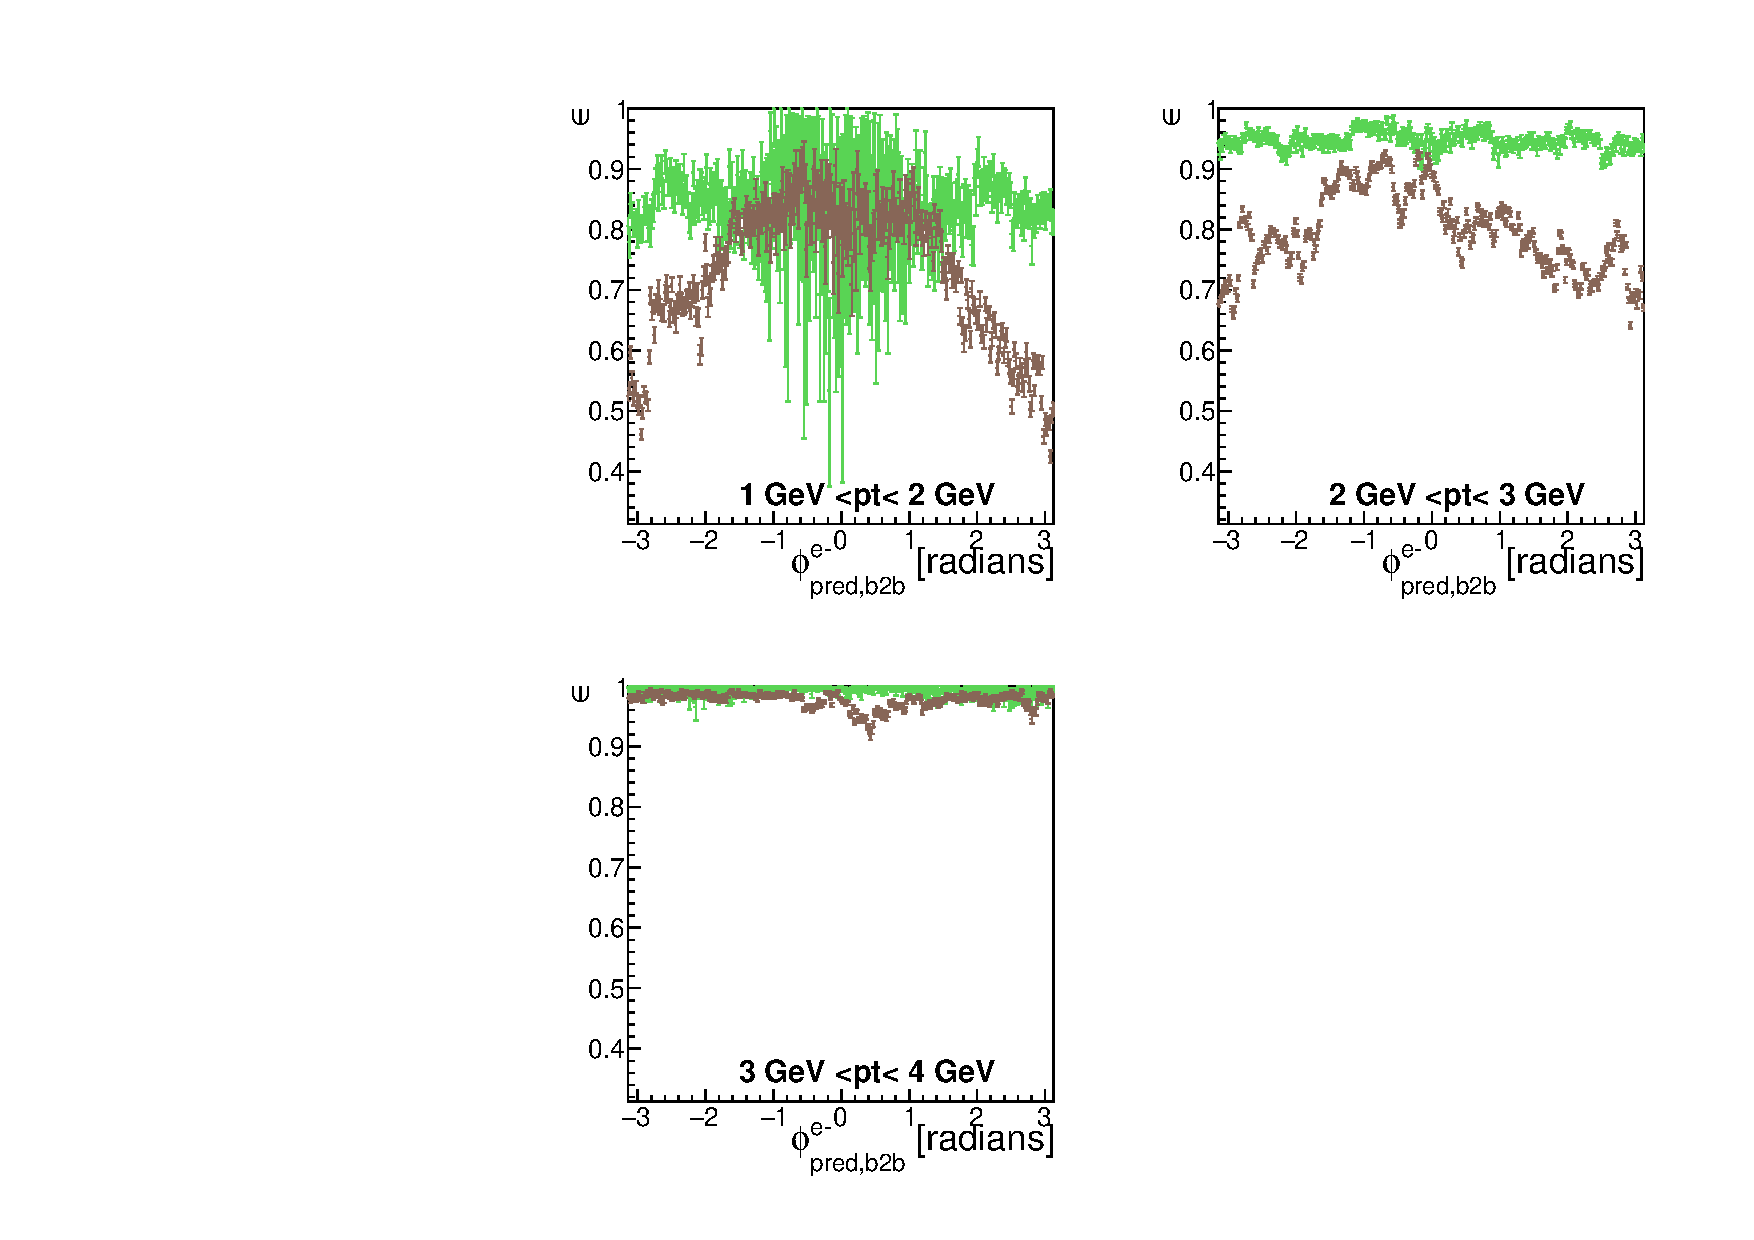
\includegraphics[width=\textwidth]{VPlots/P2/xPtMPhiemFC}
	\end{textblock*}
	
	\begin{textblock*}{2cm}(2.3cm,-3.5cm)
		$\textrm{e}^-$
	\end{textblock*}
	
	\begin{textblock*}{2cm}(8.7cm,-3.5cm)
		$\textrm{e}^+$
	\end{textblock*}
	
	
	\begin{textblock*}{11cm}(5.5cm,-4.3cm)
		
		\begin{center}
			\line(0,1){256}
		\end{center}
		
	\end{textblock*}
	
	
	\begin{textblock*}{6.5cm}(6cm,-2.5cm)
		
		\setlength{\unitlength}{5cm}
		\begin{picture}(1,1)
		\put(0,0){\line(1,1){1}}
		
		\end{picture}
		
	\end{textblock*}
	
	
	
	\begin{textblock*}{4cm}(-0.5cm,-3.7cm)
		\textcolor{OliveGreen}{Phase2 MC10}
		
		\textcolor{brown}{Phase2 Data}
	\end{textblock*}
	
	
	
	
	
	
	
	
\end{frame}

\begin{frame}{Phase2 pt Tracking Efficiencies As Function Of $\phi_{\textrm{pred,b2b}}$; Barrel}
	
	
	\begin{textblock*}{6.5cm}(-0.9cm,-3cm)
		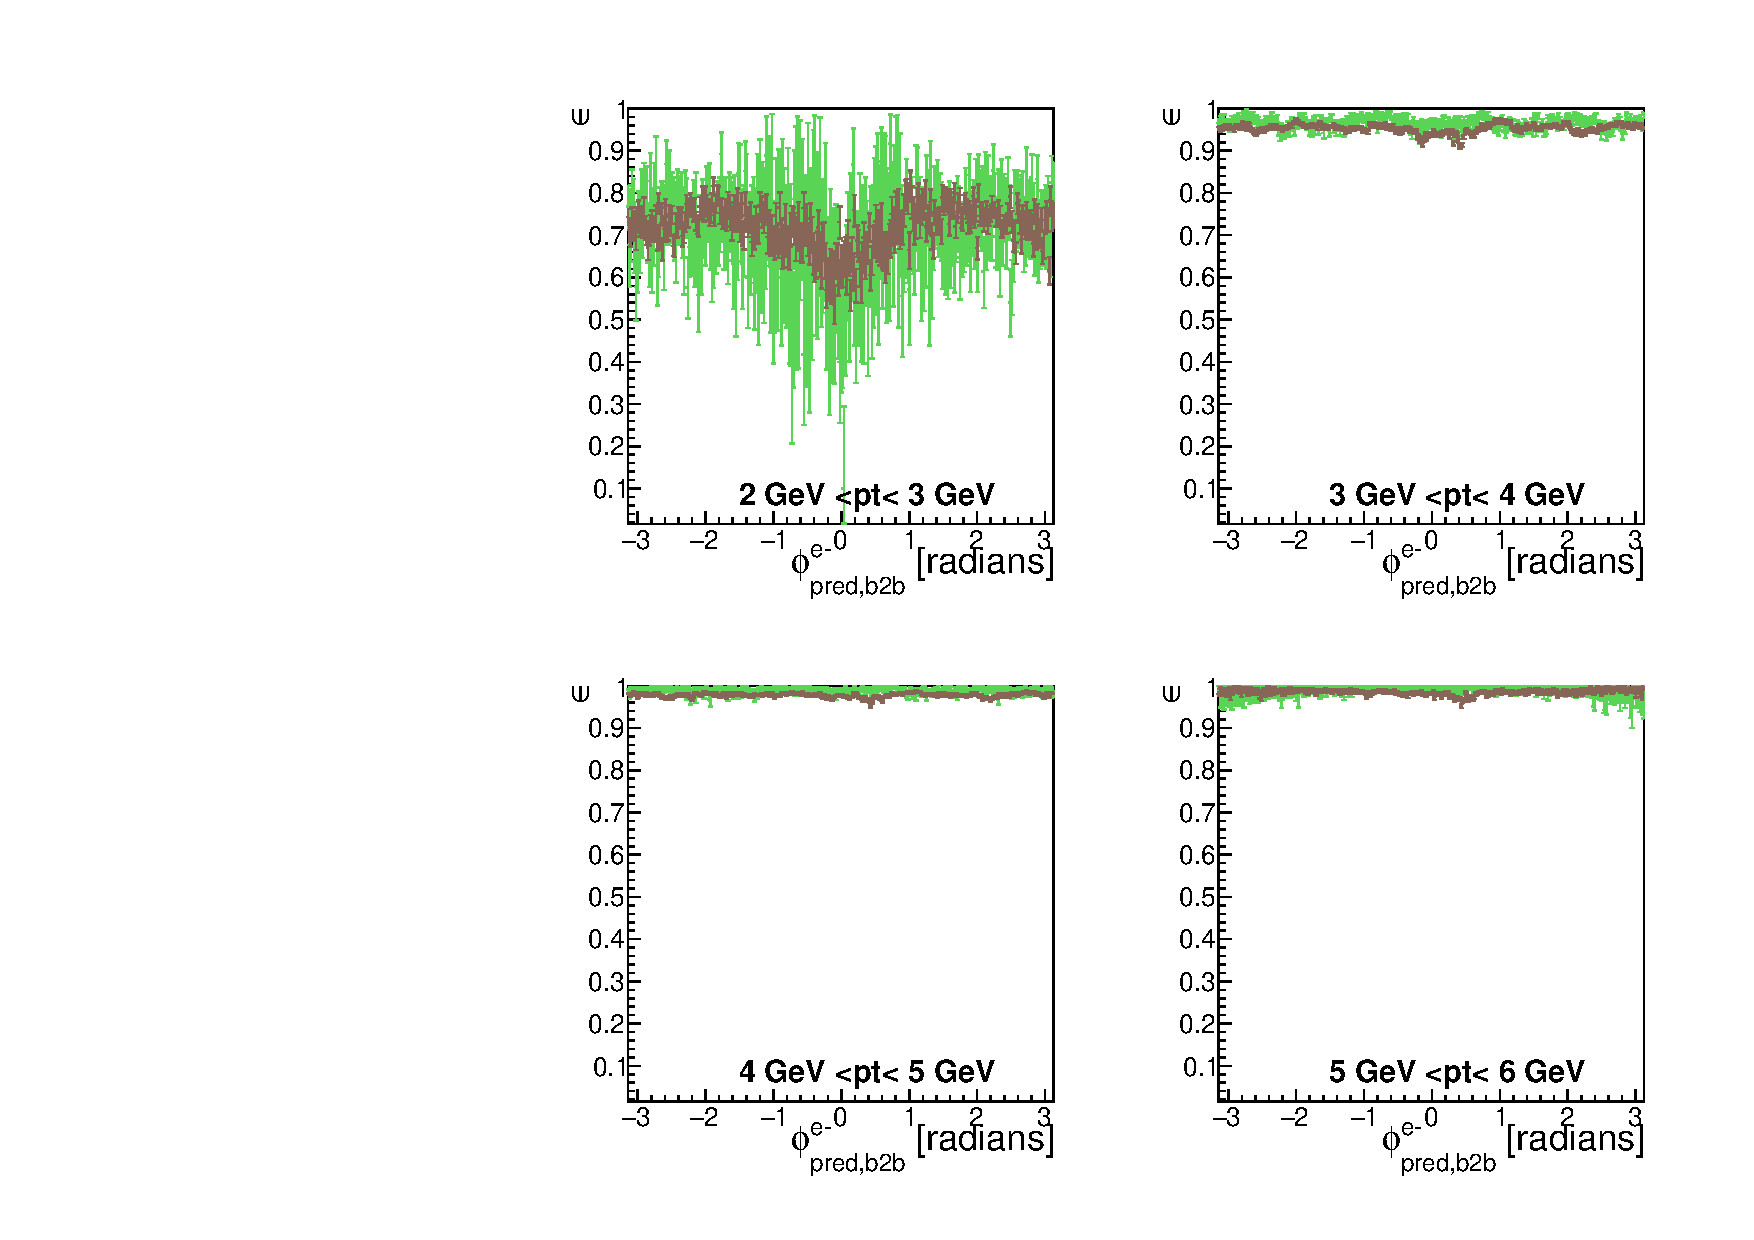
\includegraphics[width=\textwidth]{VPlots/P2/xPtMPhiemBarrel}
	\end{textblock*}
	
	\begin{textblock*}{6.5cm}(5.5cm,-3cm)
		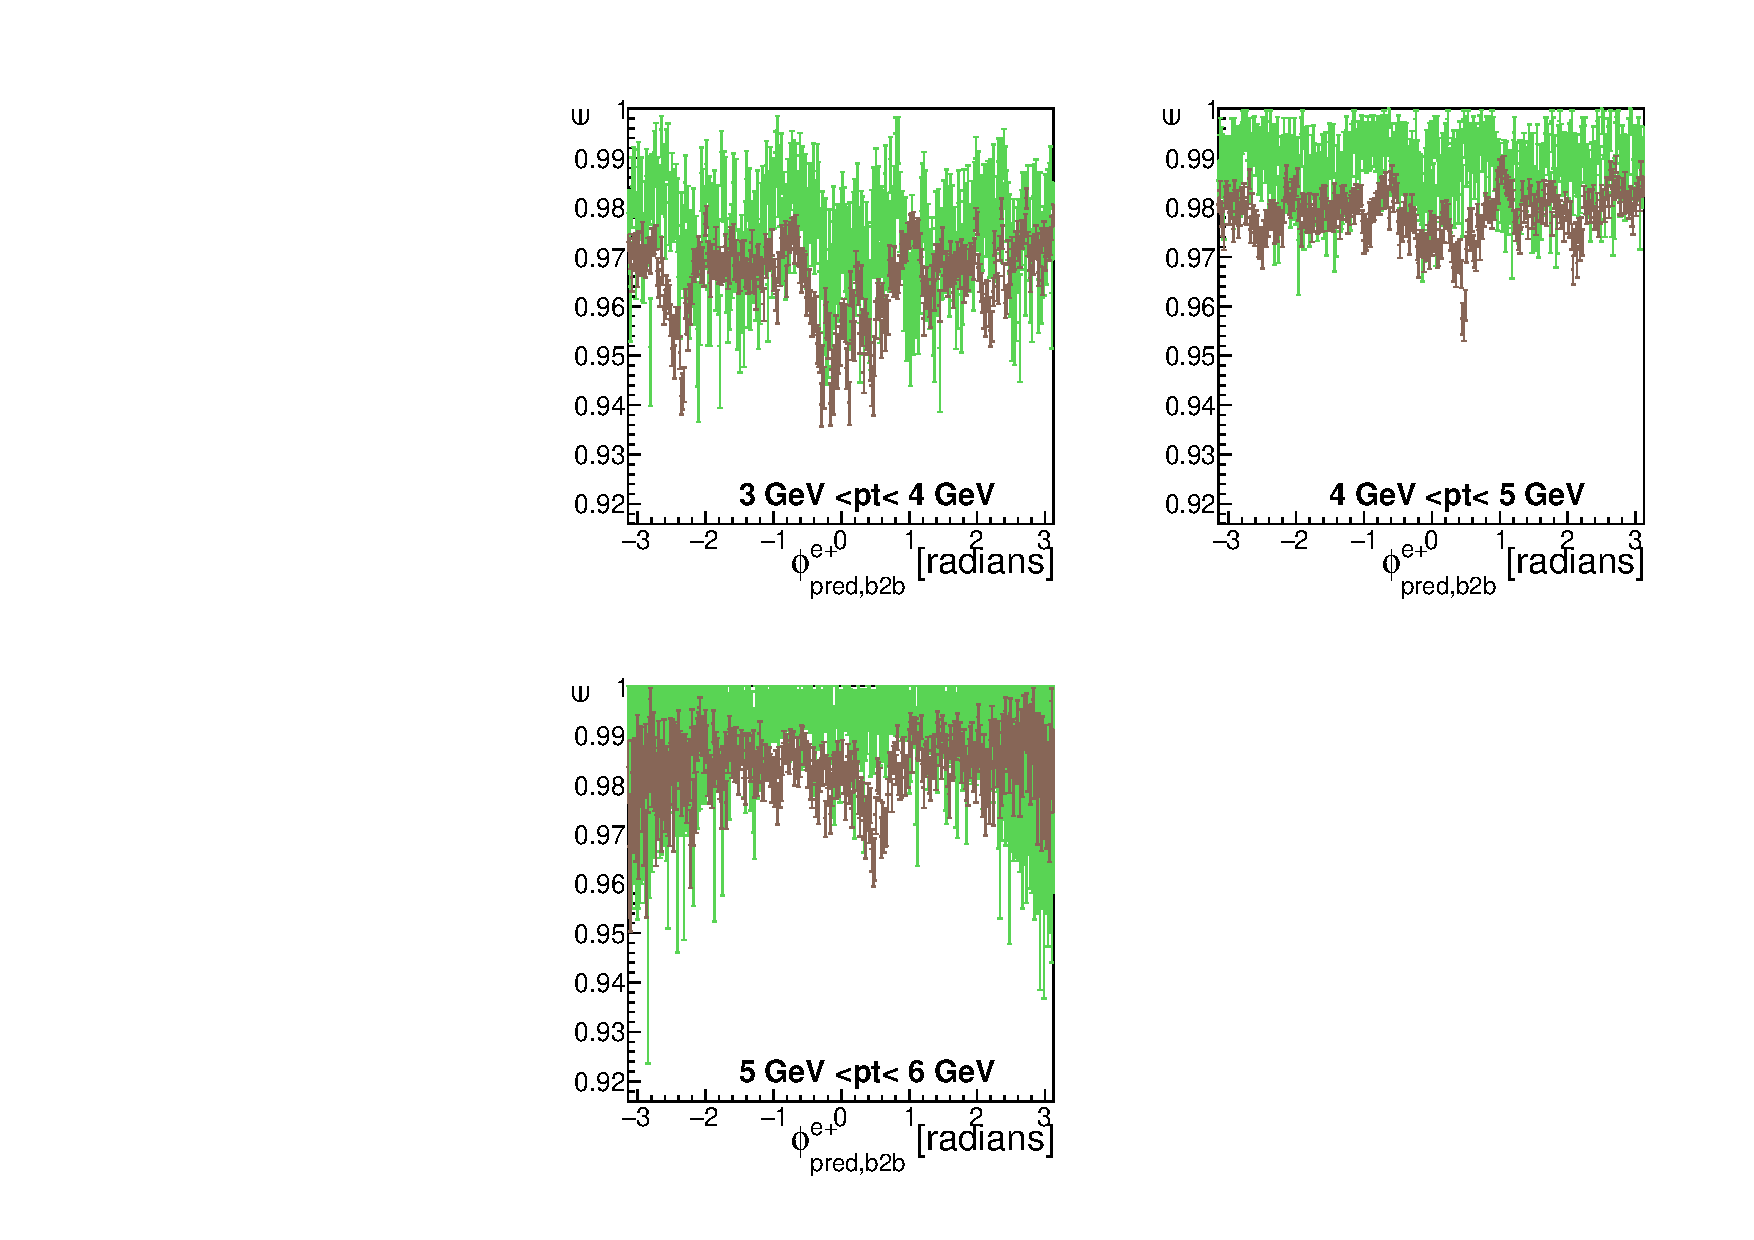
\includegraphics[width=\textwidth]{VPlots/P2/xPtMPhiepBarrel}
	\end{textblock*}
	
	
	\begin{textblock*}{2cm}(2.3cm,-3.5cm)
		$\textrm{e}^-$
	\end{textblock*}
	
	\begin{textblock*}{2cm}(8.7cm,-3.5cm)
		$\textrm{e}^+$
	\end{textblock*}
	
	
	
	\begin{textblock*}{11cm}(5.5cm,-4.3cm)
		
		\begin{center}
			\line(0,1){256}
		\end{center}
		
	\end{textblock*}
	
	
	
	\begin{textblock*}{4cm}(-0.5cm,-3.7cm)
		\textcolor{OliveGreen}{Phase2 MC10}
		
		\textcolor{brown}{Phase2 Data}
	\end{textblock*}
	
	
	
	
\end{frame}



\begin{frame}{Phase2 pt Tracking Efficiencies As Function Of $\phi_{\textrm{pred,b2b}}$; Backward End-Cap}
	
	
	\begin{textblock*}{6.5cm}(5.5cm,-3cm)
		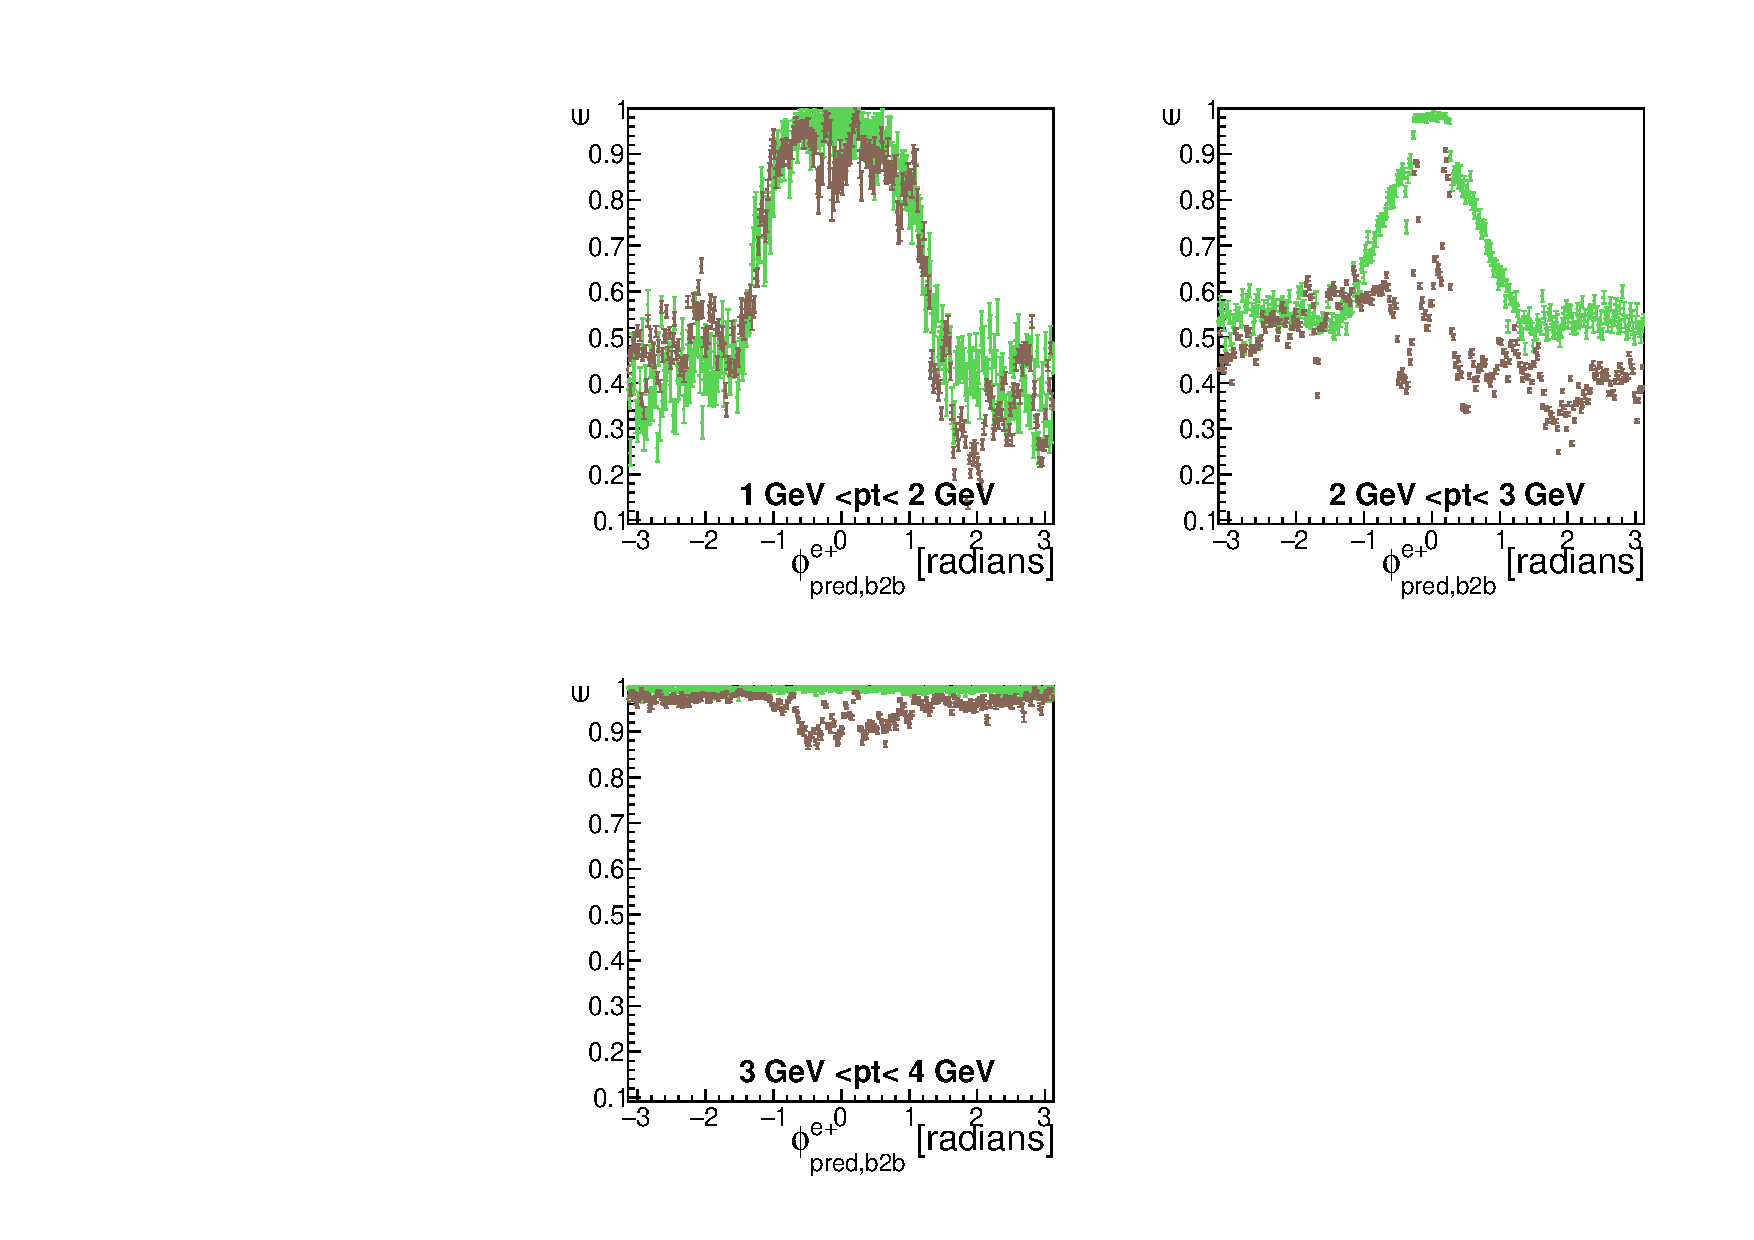
\includegraphics[width=\textwidth]{VPlots/P2/xPtMPhiepEC}
	\end{textblock*}
	
	\begin{textblock*}{2cm}(2.3cm,-3.5cm)
		$\textrm{e}^-$
	\end{textblock*}
	
	\begin{textblock*}{2cm}(8.7cm,-3.5cm)
		$\textrm{e}^+$
	\end{textblock*}
	
	
	\begin{textblock*}{11cm}(5.5cm,-4.3cm)
		
		\begin{center}
			\line(0,1){256}
		\end{center}
		
	\end{textblock*}
	
	
	\begin{textblock*}{6.5cm}(-0.2cm,-2.5cm)
		
		\setlength{\unitlength}{5cm}
		\begin{picture}(1,1)
		\put(0,0){\line(1,1){1}}
		
		\end{picture}
		
	\end{textblock*}
	
	\begin{textblock*}{4cm}(-0.5cm,-3.7cm)
		\textcolor{OliveGreen}{Phase2 MC10}
		
		\textcolor{brown}{Phase2 Data}
	\end{textblock*}
	
\end{frame}


\begin{frame}{Phase2 pt Tracking Efficiencies As Function Of $\theta_{\textrm{pred,b2b}}$}
	
	
	\begin{textblock*}{6.5cm}(-0.9cm,-3cm)
		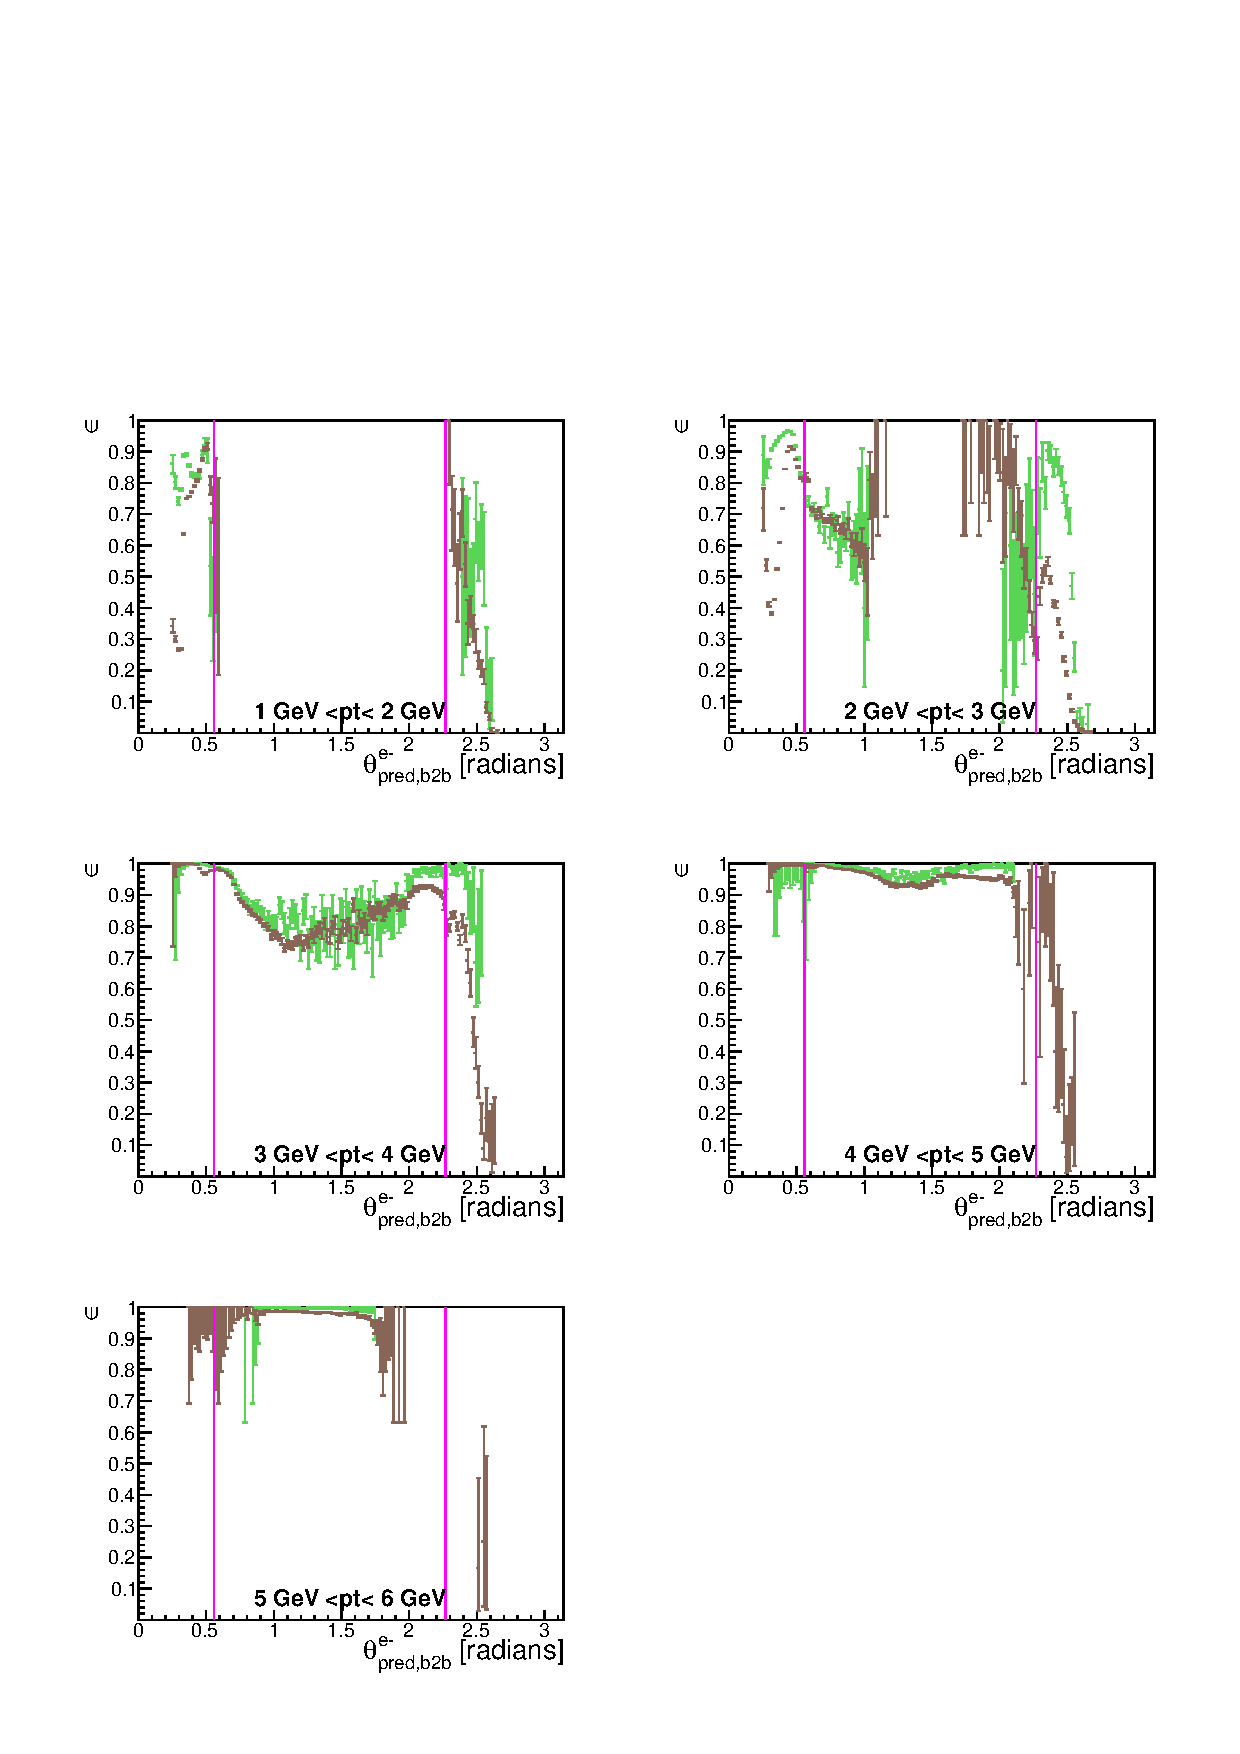
\includegraphics[width=\textwidth]{VPlots/P2/xPtMThetaem}
	\end{textblock*}
	
	\begin{textblock*}{6.5cm}(5.5cm,-3cm)
		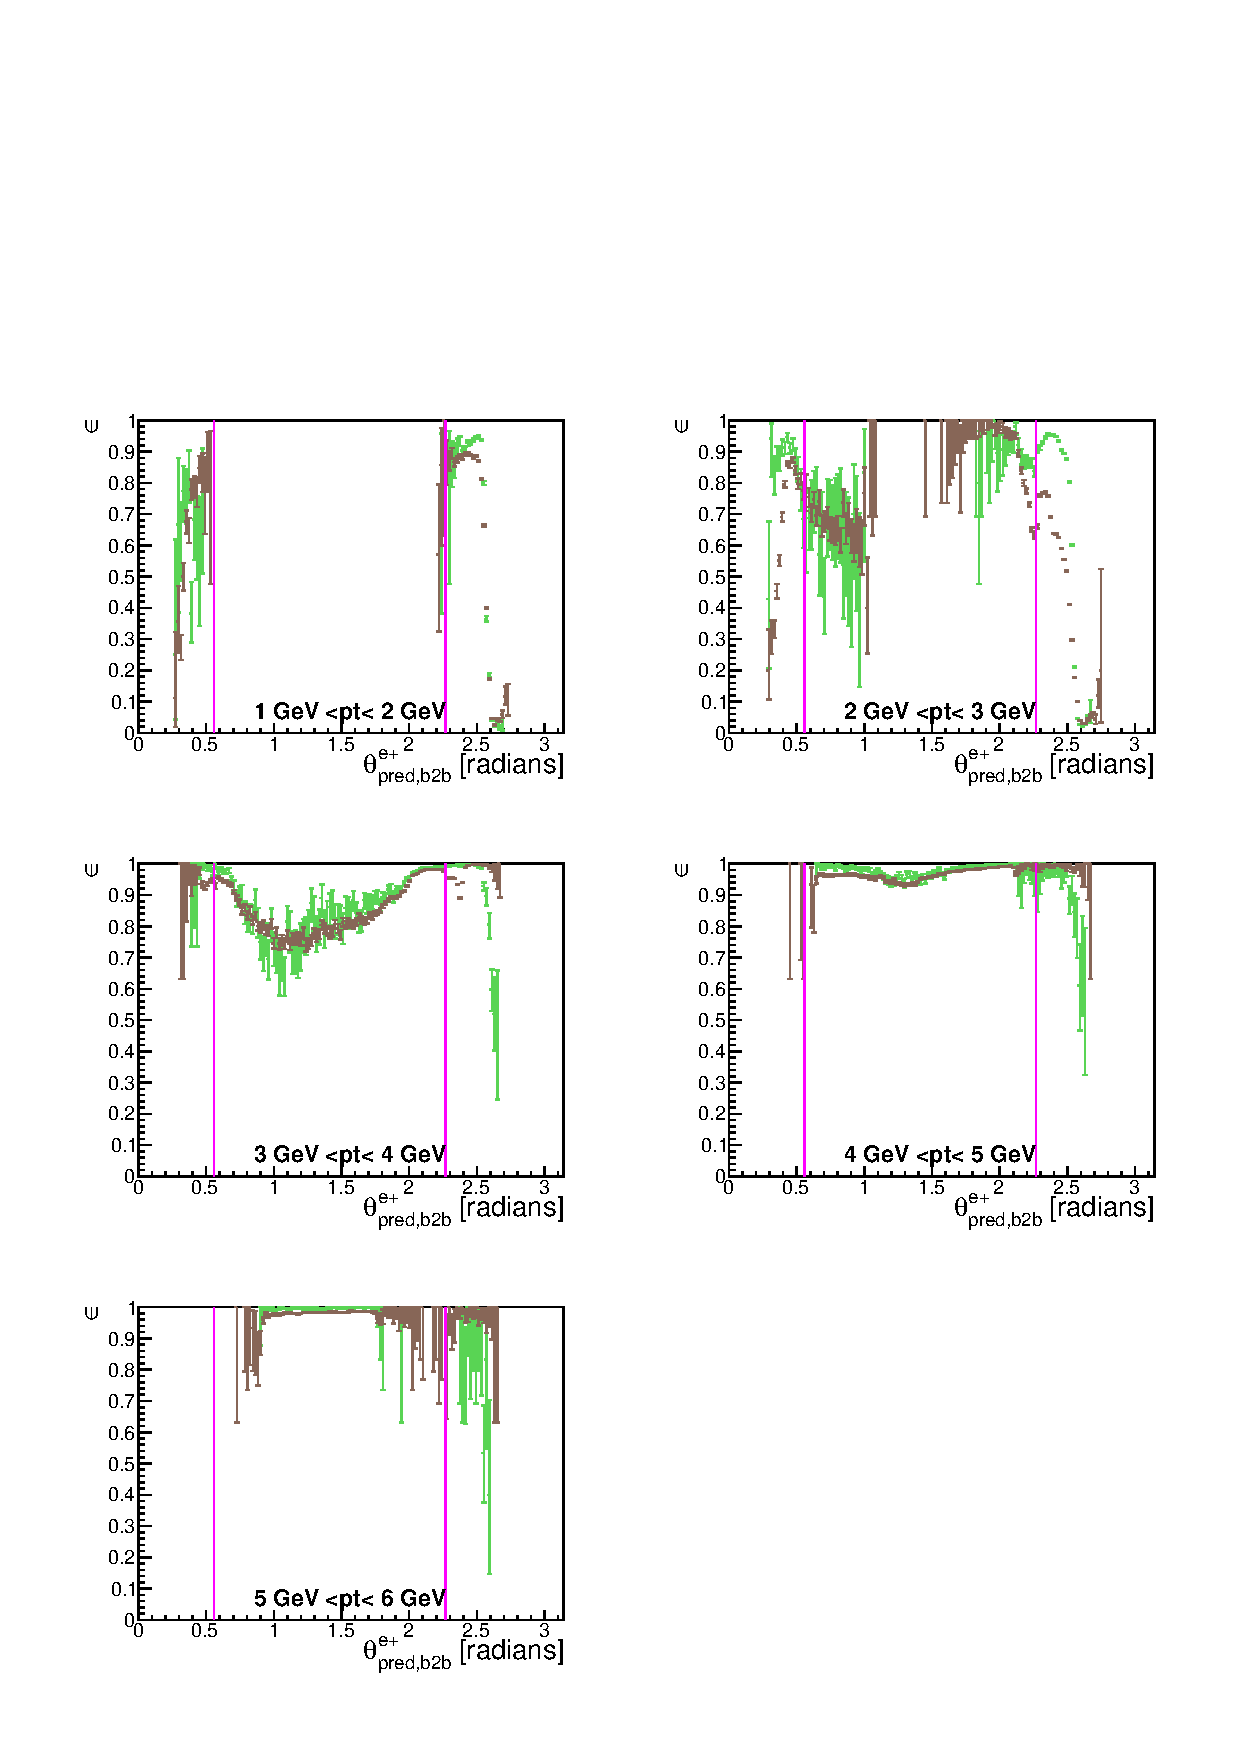
\includegraphics[width=\textwidth]{VPlots/P2/xPtMThetaep}
	\end{textblock*}
	
	
	\begin{textblock*}{2cm}(2.3cm,-3.5cm)
		$\textrm{e}^-$
	\end{textblock*}
	
	\begin{textblock*}{2cm}(8.7cm,-3.5cm)
		$\textrm{e}^+$
	\end{textblock*}
	
	
	
	\begin{textblock*}{11cm}(5.5cm,-4.3cm)
		
		\begin{center}
			\line(0,1){256}
		\end{center}
		
	\end{textblock*}
	
	\begin{textblock*}{4cm}(-0.5cm,-3.7cm)
		\textcolor{OliveGreen}{Phase2 MC10}
		
		\textcolor{brown}{Phase2 Data}
	\end{textblock*}
	
	
	
	
	
\end{frame}














\begin{frame}{Phase3 pt Tracking Efficiencies As Function Of $\phi_{\textrm{pred,b2b}}$; Forward End-Cap}
	
	
	\begin{textblock*}{6.5cm}(-0.9cm,-3cm)
		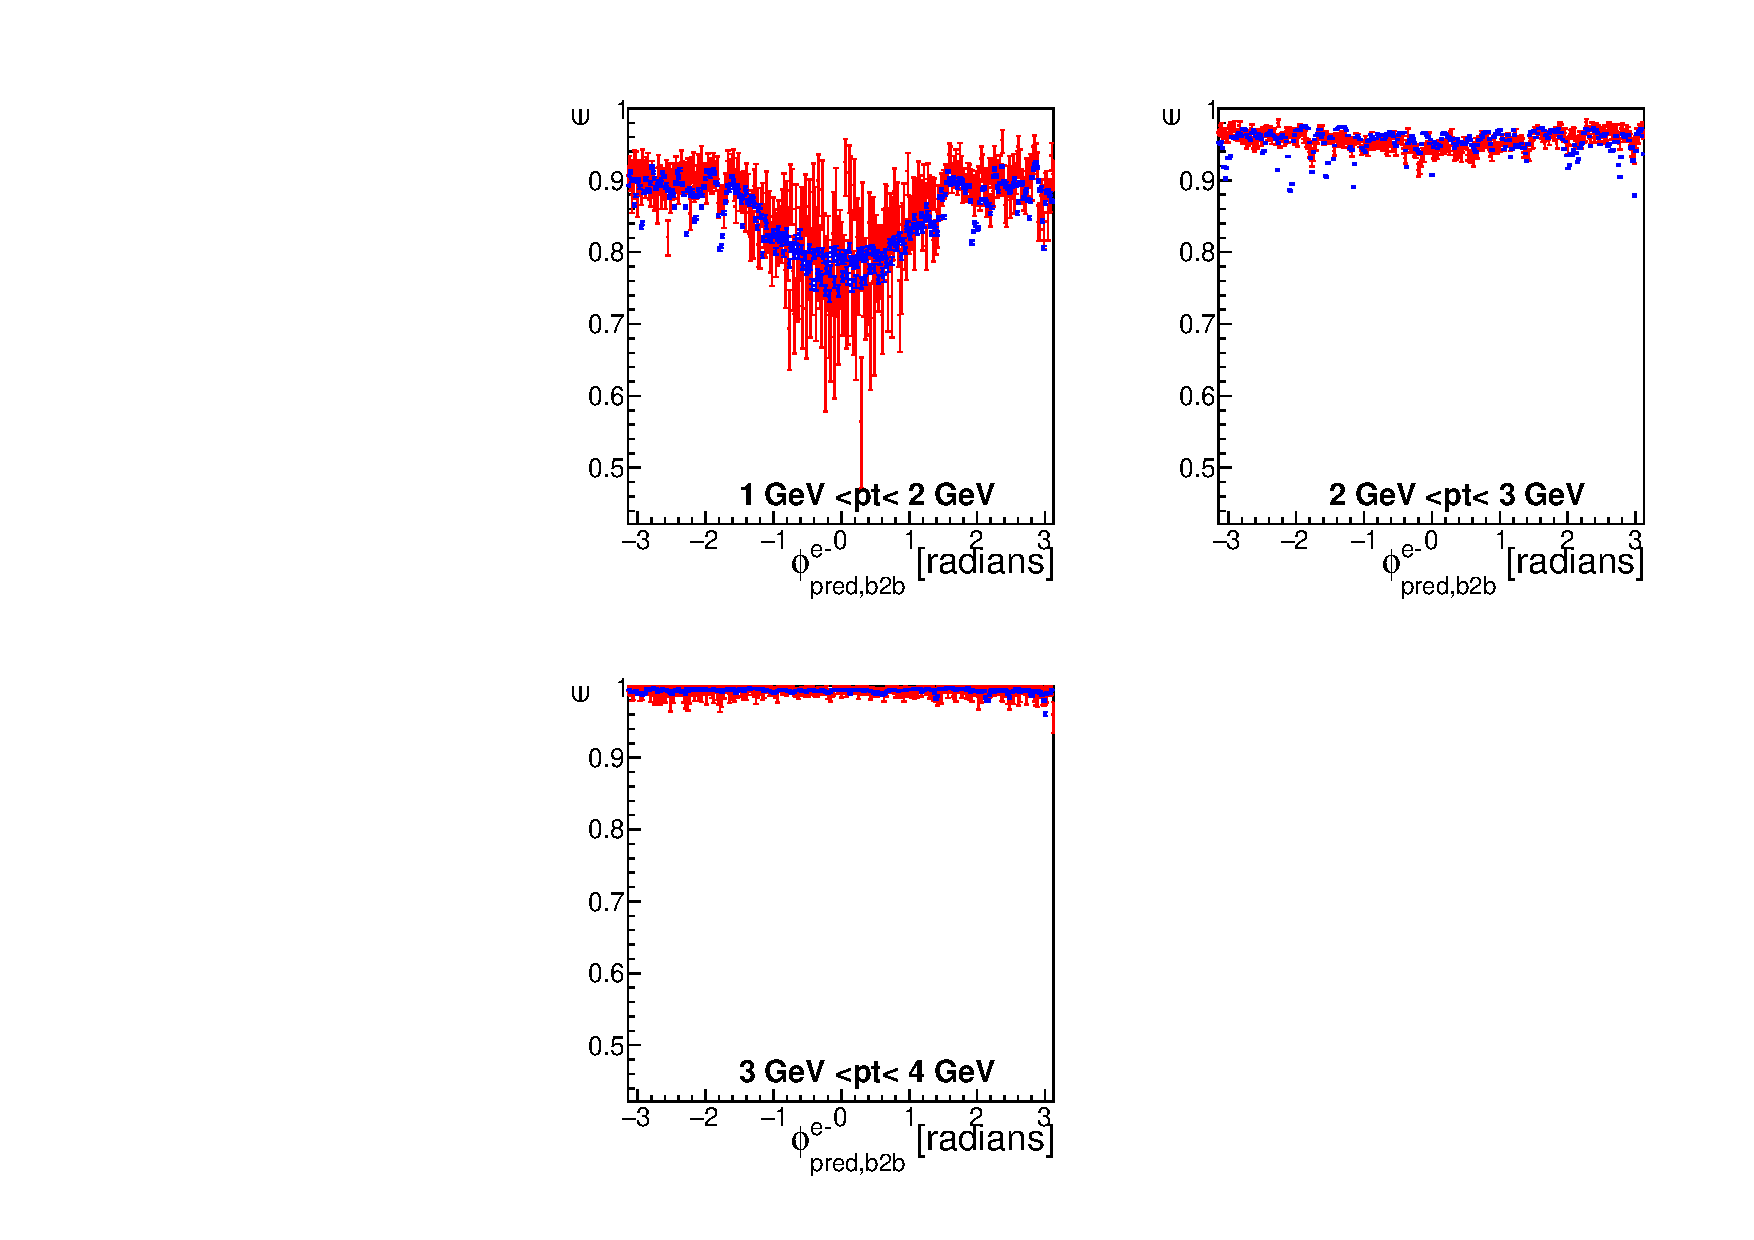
\includegraphics[width=\textwidth]{VPlots/P3/xPtMPhiemFCP3}
	\end{textblock*}
	
	\begin{textblock*}{2cm}(2.3cm,-3.5cm)
		$\textrm{e}^-$
	\end{textblock*}
	
	\begin{textblock*}{2cm}(8.7cm,-3.5cm)
		$\textrm{e}^+$
	\end{textblock*}
	
	
	\begin{textblock*}{11cm}(5.5cm,-4.3cm)
		
		\begin{center}
			\line(0,1){256}
		\end{center}
		
	\end{textblock*}
	
	
	\begin{textblock*}{6.5cm}(6cm,-2.5cm)
		
		\setlength{\unitlength}{5cm}
		\begin{picture}(1,1)
		\put(0,0){\line(1,1){1}}
		
		\end{picture}
		
	\end{textblock*}
	
	
	
	\begin{textblock*}{4cm}(-0.5cm,-3.7cm)
		\textcolor{red}{Phase3 MC10}
		
		\textcolor{blue}{Phase3 Data}
	\end{textblock*}
	
	
	
	
	
	
	
	
\end{frame}

\begin{frame}{Phase3 pt Tracking Efficiencies As Function Of $\phi_{\textrm{pred,b2b}}$; Barrel}
	
	
	\begin{textblock*}{6.5cm}(-0.9cm,-3cm)
		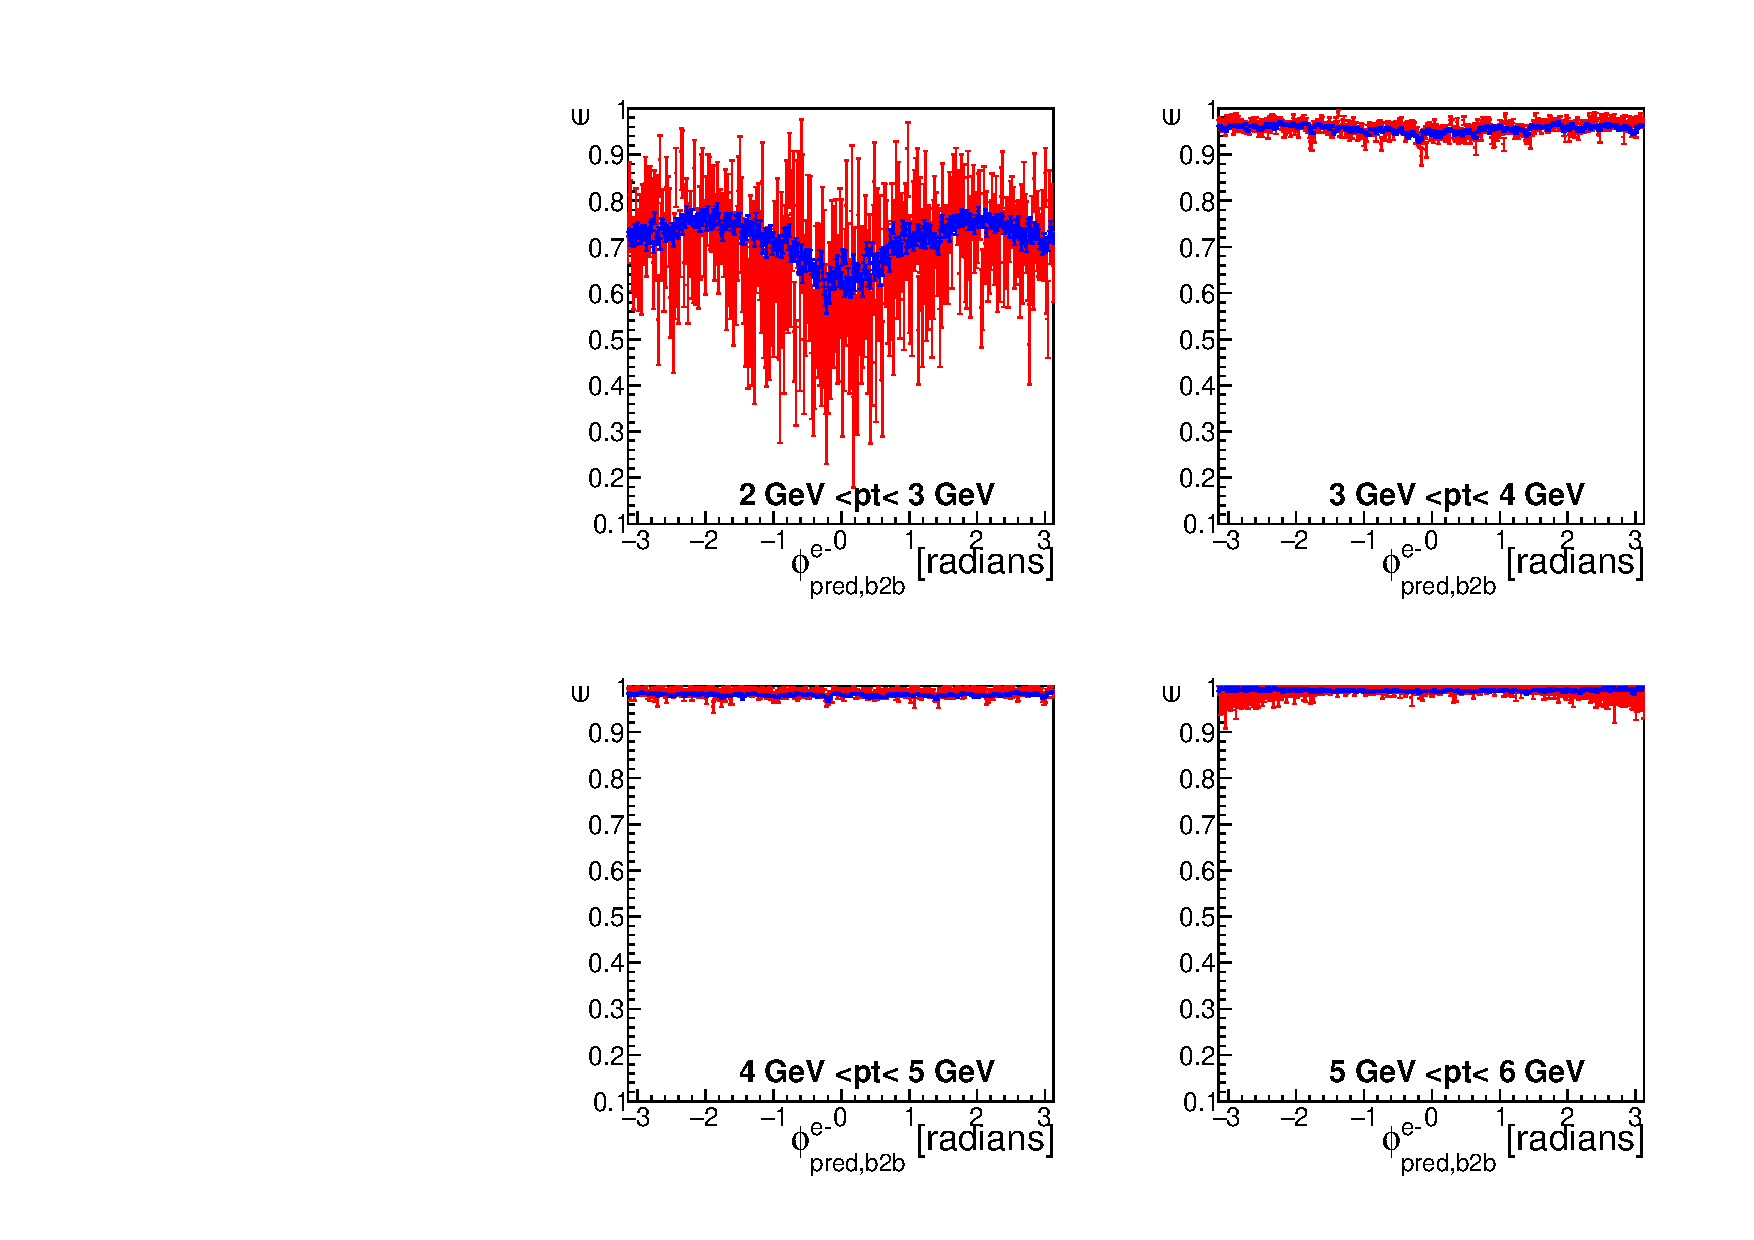
\includegraphics[width=\textwidth]{VPlots/P3/xPtMPhiemBarrelP3}
	\end{textblock*}
	
	\begin{textblock*}{6.5cm}(5.5cm,-3cm)
		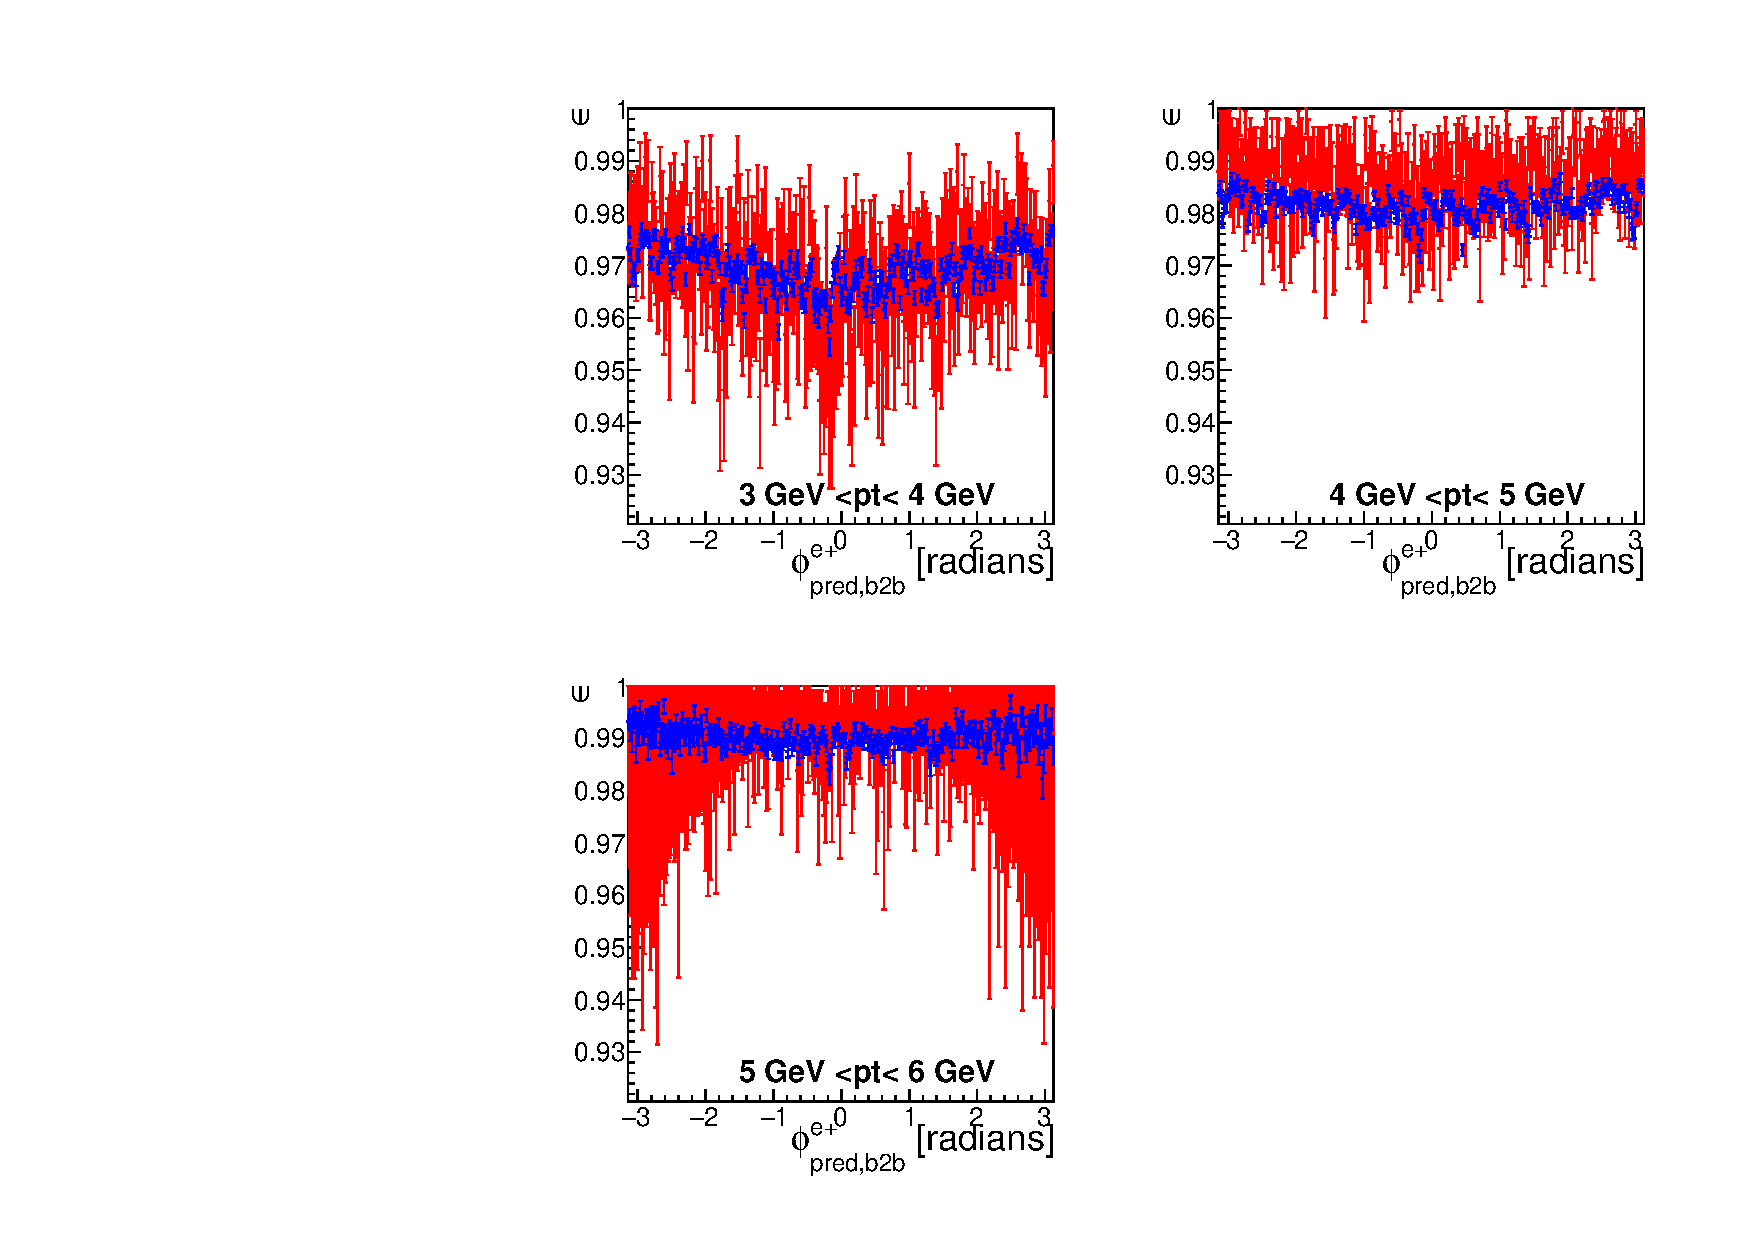
\includegraphics[width=\textwidth]{VPlots/P3/xPtMPhiepBarrelP3}
	\end{textblock*}
	
	
	\begin{textblock*}{2cm}(2.3cm,-3.5cm)
		$\textrm{e}^-$
	\end{textblock*}
	
	\begin{textblock*}{2cm}(8.7cm,-3.5cm)
		$\textrm{e}^+$
	\end{textblock*}
	
	
	
	\begin{textblock*}{11cm}(5.5cm,-4.3cm)
		
		\begin{center}
			\line(0,1){256}
		\end{center}
		
	\end{textblock*}
	
	
	
	\begin{textblock*}{4cm}(-0.5cm,-3.7cm)
		\textcolor{red}{Phase3 MC10}
		
		\textcolor{blue}{Phase3 Data}
	\end{textblock*}
	
	
	
	
\end{frame}



\begin{frame}{Phase3 pt Tracking Efficiencies As Function Of $\phi_{\textrm{pred,b2b}}$; Backward End-Cap}
	
	
	\begin{textblock*}{6.5cm}(5.5cm,-3cm)
		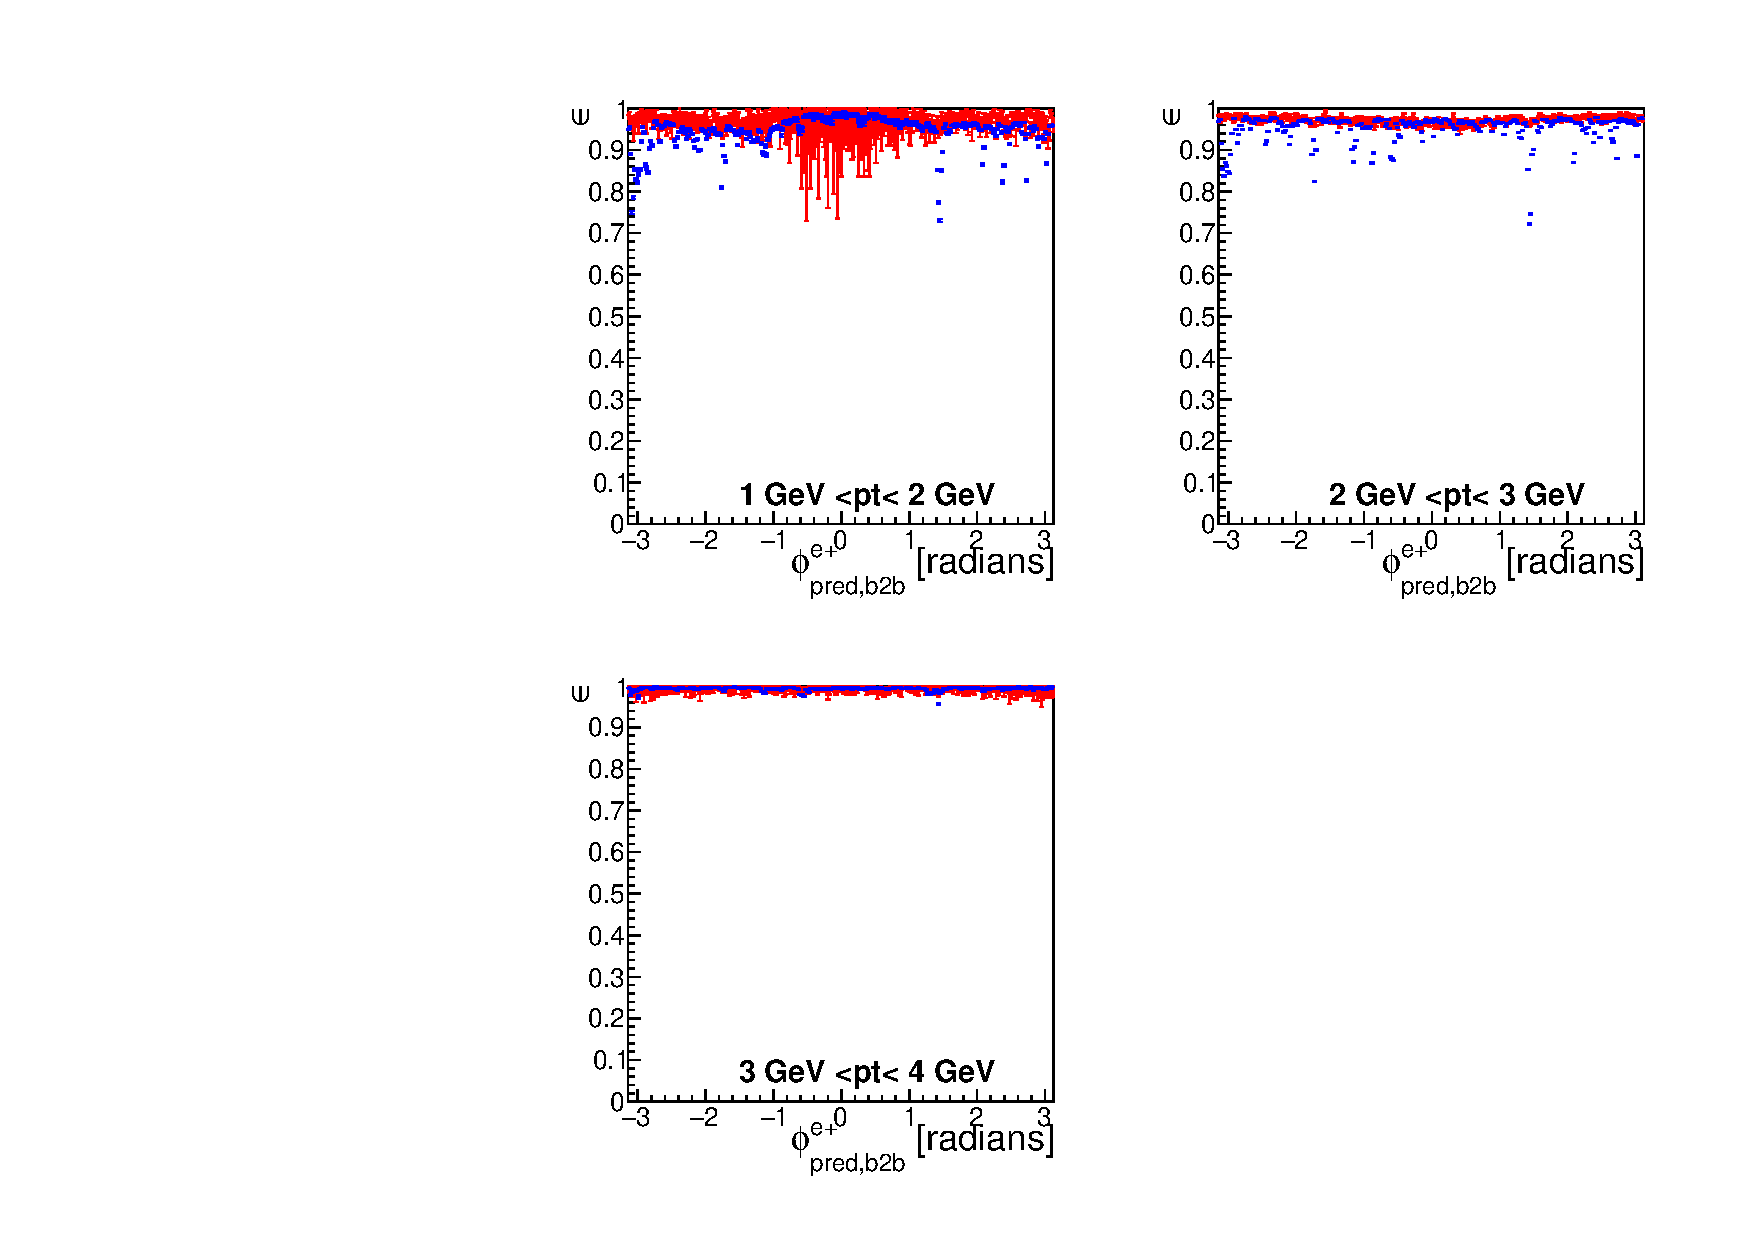
\includegraphics[width=\textwidth]{VPlots/P3/xPtMPhiepECP3}
	\end{textblock*}
	
	\begin{textblock*}{2cm}(2.3cm,-3.5cm)
		$\textrm{e}^-$
	\end{textblock*}
	
	\begin{textblock*}{2cm}(8.7cm,-3.5cm)
		$\textrm{e}^+$
	\end{textblock*}
	
	
	\begin{textblock*}{11cm}(5.5cm,-4.3cm)
		
		\begin{center}
			\line(0,1){256}
		\end{center}
		
	\end{textblock*}
	
	
	\begin{textblock*}{6.5cm}(-0.2cm,-2.5cm)
		
		\setlength{\unitlength}{5cm}
		\begin{picture}(1,1)
		\put(0,0){\line(1,1){1}}
		
		\end{picture}
		
	\end{textblock*}
	
	\begin{textblock*}{4cm}(-0.5cm,-3.7cm)
		\textcolor{red}{Phase3 MC10}
		
		\textcolor{blue}{Phase3 Data}
	\end{textblock*}
	
\end{frame}


\begin{frame}{Phase3 pt Tracking Efficiencies As Function Of $\theta_{\textrm{pred,b2b}}$}
	
	
	\begin{textblock*}{6.5cm}(-0.9cm,-3cm)
		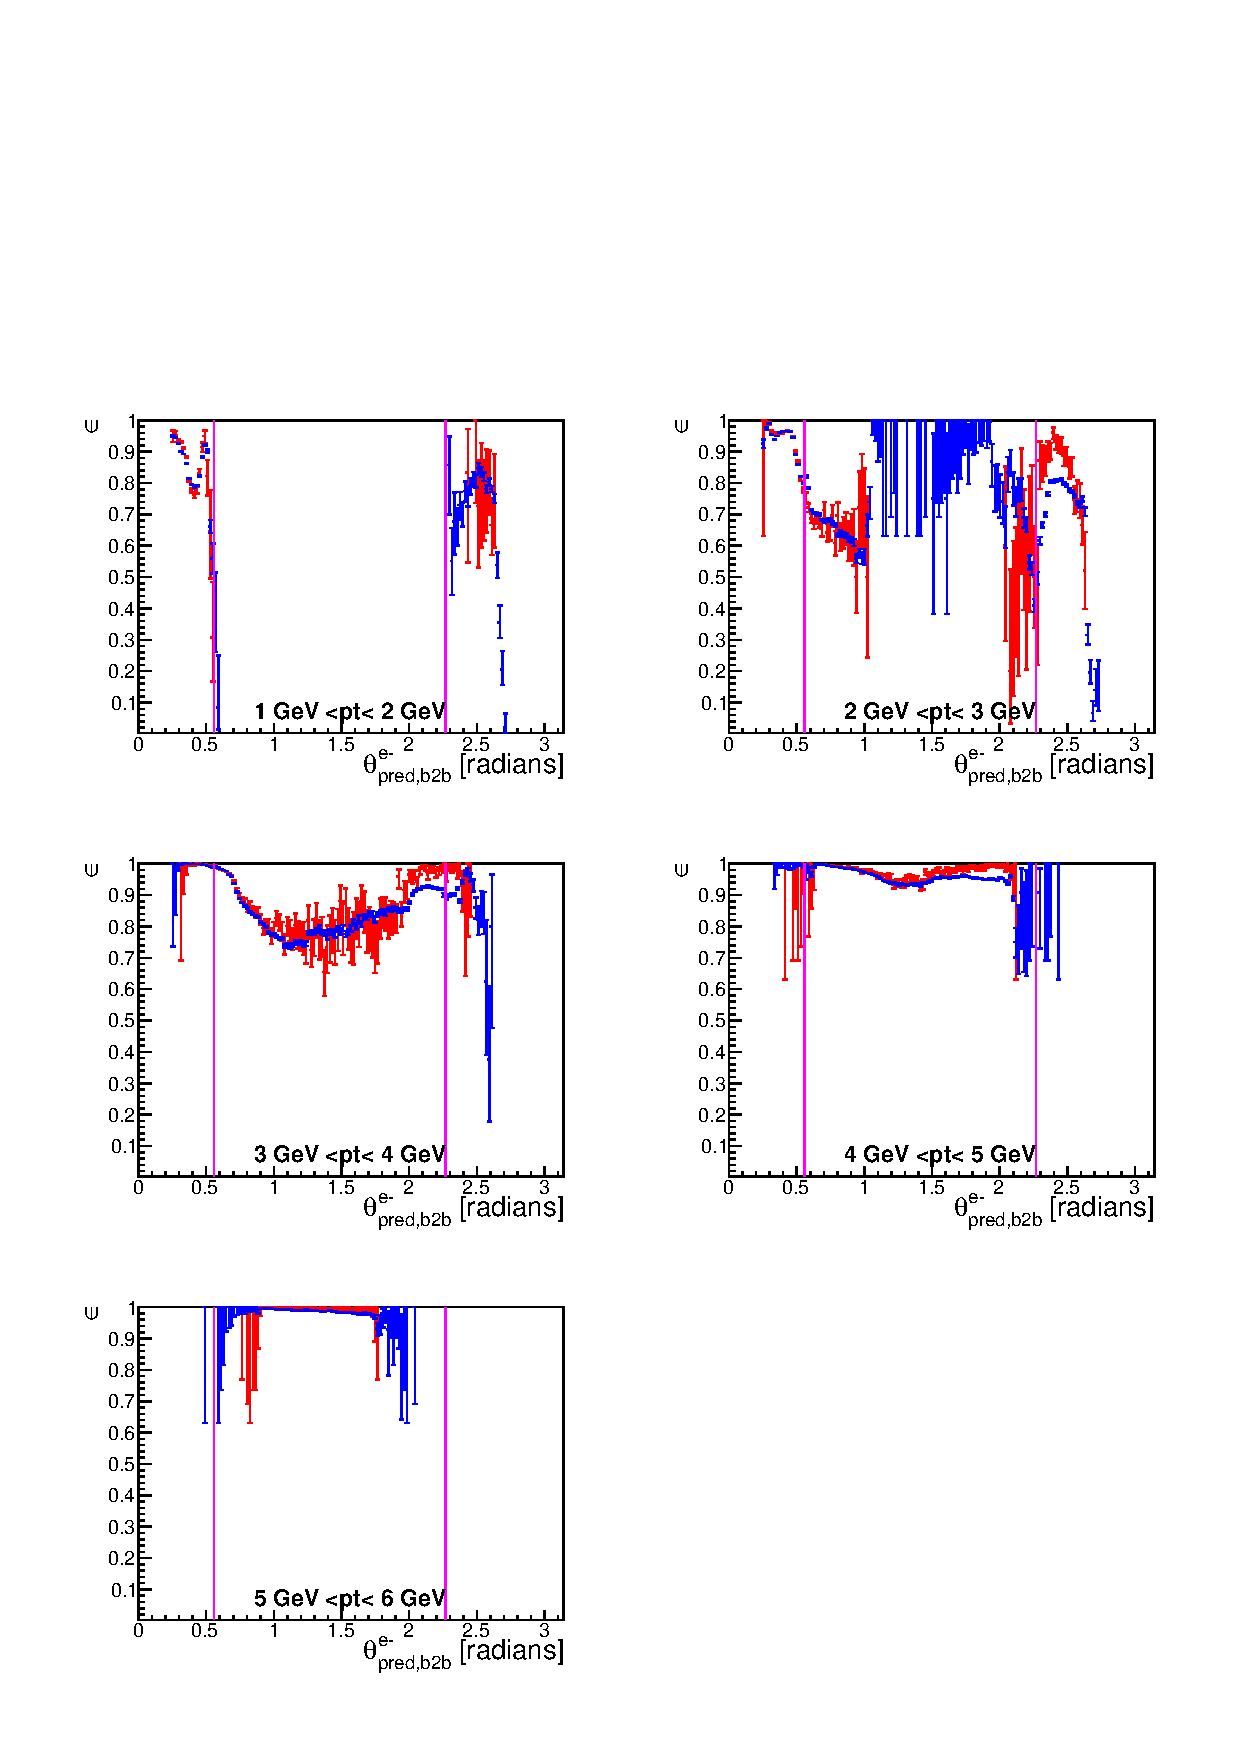
\includegraphics[width=\textwidth]{VPlots/P3/xPtMThetaemP3}
	\end{textblock*}
	
	\begin{textblock*}{6.5cm}(5.5cm,-3cm)
		\includegraphics[width=\textwidth]{VPlots/P3/xPtMThetaepP3}
	\end{textblock*}
	
	
	\begin{textblock*}{2cm}(2.3cm,-3.5cm)
		$\textrm{e}^-$
	\end{textblock*}
	
	\begin{textblock*}{2cm}(8.7cm,-3.5cm)
		$\textrm{e}^+$
	\end{textblock*}
	
	
	
	\begin{textblock*}{11cm}(5.5cm,-4.3cm)
		
		\begin{center}
			\line(0,1){256}
		\end{center}
		
	\end{textblock*}
	
	\begin{textblock*}{4cm}(-0.5cm,-3.7cm)
		\textcolor{red}{Phase3 MC10}
		
		\textcolor{blue}{Phase3 Data}
	\end{textblock*}
	




\end{frame}





\end{document}
